\documentclass[11pt,a4paper,twoside]{tesis}
% \documentclass[11pt,a4paper]{tesis}

\usepackage{graphicx}
\usepackage[utf8]{inputenc}
\usepackage{babelbib}
\usepackage[spanish]{babel}
\usepackage[left=2.5cm,right=2.5cm,bottom=3.5cm,top=3.5cm]{geometry}
\usepackage[font=small,labelfont=bf]{caption} % Required for specifying captions to tables and figures
\usepackage{color}
\usepackage{epigraph}
\usepackage{float}
\usepackage{titlesec}
\usepackage{upgreek}
\usepackage{url}
\usepackage{caption}
\usepackage{subcaption,mwe}
\usepackage{longtable}
\usepackage{listings}
\usepackage{amsmath}
\usepackage{dirtree}
\usepackage{xcolor}
\usepackage{multicol}
\usepackage{hyperref}

\newcommand\todo[1]{\textcolor{red}{#1}}
\newcommand\myicon[1]{{\color{#1}\rule{2ex}{2ex}}}
\newcommand{\myfolder}[2]{\myicon{#1}\ {#2}}

\begin{document}

%%%% CARATULA
\def\titulo{Licenciado}
\def\autor{Martín Ezequiel Langberg}
\def\tituloTesis{Predicción de patogenicidad en SNPs usando aprendizaje automático}
\def\runtitulo{Predicción de patogenicidad en polimorfismos de un solo nucleótido usando aprendizaje automático}
\def\director{Ariel Berenstein}
\def\codirector{Pablo Turjanski}
\def\lugar{Buenos Aires, 2019}
\newcommand{\HRule}{\rule{\linewidth}{0.2mm}}
%
\thispagestyle{empty}

\begin{center}\leavevmode

\vspace{-2cm}

\begin{tabular}{l}

\includegraphics[width=2.6cm]{logofcen.pdf}
\end{tabular}


{\large \sc Universidad de Buenos Aires

Facultad de Ciencias Exactas y Naturales

Departamento de Computaci\'on}

\vspace{6.0cm}

%\vspace{3.0cm}
%{
%\Large \color{red}
%\begin{tabular}{|p{2cm}cp{2cm}|}
%\hline
%& Pre-Final Version: \today &\\
%\hline
%\end{tabular}
%}
%\vspace{2.5cm}

\begin{huge}
\textbf{\tituloTesis}
\end{huge}

\vspace{2cm}

{\large Tesis de Licenciatura en Ciencias de la Computaci\'on}

\vspace{2cm}

{\Large \autor}

\end{center}

\vfill

{\large

{Director: \director}

\vspace{.2cm}

{Codirector: \codirector}

\vspace{.2cm}

\lugar
}

\newpage\thispagestyle{empty}


%%%% ABSTRACTS, AGRADECIMIENTOS Y DEDICATORIA
\frontmatter
\pagestyle{empty}
%\begin{center}
%\large \bf \runtitulo
%\end{center}
%\vspace{1cm}
\chapter*{\runtitulo}

\noindent La predicción de enfermedades causadas por los polimorfismos de un solo nucleótido (SNPs, por sus siglas en inglés) tuvo un desarrollo constante y acelerado en los últimos años en parte gracias a nuevas técnicas de secuenciación del genoma, que permite el análisis del material genético de pacientes con mayor facilidad. Nuestro objetivo es generar un método de predicción propio a través del análisis de distintas herramientas ya existentes, reutilizando sus features más importantes, como así también agregando nuevos y explorando distintos métodos de Aprendizaje Automático que superen las métricas alcanzadas por los trabajos previos en el área.

\bigskip

\noindent\textbf{Palabras claves:} Aprendizaje Automático, Bioinformática, SNPs, Patogenicidad, Genética.

% \cleardoublepage
% %\begin{center}
%\large \bf \runtitle
%\end{center}
%\vspace{1cm}
\chapter*{\runtitle}

\noindent 

\bigskip

\noindent\textbf{Keywords:} . % OPCIONAL: comentar si no se quiere

% \cleardoublepage
% \chapter*{Agradecimientos}

Haber terminado esta Tesis de Licenciatura no solamente significó la culminación de un arduo período de trabajo sino que también representa el ``cierre'' formal de una etapa. Esto me invita a la reflexión sobre los momentos transitados durante todos estos años. 

Este trabajo no hubiera podido realizarse sin el acompañamiento recibido de muchas personas en diferentes momentos, y quiero aprovechar esta oportunidad para agradecer a todas aquellas que mi memoria me ayuda a recordar.  

A mi familia: Mis padres, hermanos, tíos, primos y abuelos. Gracias por el apoyo y el amor recibido. Especialmente a mi abuela Nelly y a mi abuela Rechel, que ya no están. Fueron mis primeras profesoras y el amor infinito que me dieron es algo que me acompaña y me da fuerzas todos los días. Se que se alegrarían muchísimo por este logro. 

A mi primer grupo de amigos durante la cursada del CBC: A Lucas y a Diego. Recuerdo con mucha felicidad haberlos tenido como compañeros en ese primer paso. Si bien después nuestros caminos se separaron, fue muy importante ese primer año de temores y éxitos compartidos.

A mis amigos eternos del secundario: Javier y Nico. Horas y horas de batallas épicas, y de campeonatos mundiales. Juntarme con ustedes siempre es el escape perfecto a otros mundos. 

A mis compañeros Mezzeteros: Ari, Javi y Gabi. Fue muy divertido haber compartido tantas materias y trabajos prácticos, pero lo mejor fue nuestro primer trabajo. Cuando llegamos a la entrevista nos confundieron con una banda de rock, y lo que siguió después fue igual de bizarro. Seguimos riéndonos de ese momento en que soñamos con ser los nuevos rockstars de la tecnología.

A mis queridos Pepes: Guille, Fixman, Luigi, Diego y JP. Estoy muy feliz y orgulloso de haber aprendido con ustedes y sobre todo de ustedes. Cómo olvidar las incontables noches comiendo pizza en el bar de deportes. Se que tengo un hogar en cualquier lugar del mundo en donde se encuentren. Quiero recordar a Leopoldo también, por haberme dado un empujón de confianza en un par de momentos importantes. Gracias, Leo.

A mis amigos del trabajo: Maxi, Yani, Pedro y Nico. Son una gran razón de mis risas durante el día a día. 

A mi gran amigo y hermano del alma Dami: Por tantas caminatas random, por los viajes y por estar siempre.

También quiero agradecer a mis directores Pablo y Ariel por todas las juntadas, por las ideas y la buena onda. En especial a Ariel por haber sido el ideólogo oficial detrás de esta ``fuga'' universitaria y en especial a Pablo por sus Vauquitas. 
Por último pero no menos importante, a la educación pública y a sus docentes por haberme acogido en cada de mis etapas de aprendizaje, me siento privilegiado y en deuda por haberme enseñado no solamente conceptos técnicos, también me ayudó a tener una conciencia social y un pensamiento crítico que me va a acompañar toda la vida.














 % OPCIONAL: comentar si no se quiere

% \cleardoublepage
% \hfill \textit{A mi persona favorita.}
  % OPCIONAL: comentar si no se quiere

\cleardoublepage
\tableofcontents

\mainmatter
\pagestyle{headings}

%%%% ACA VA EL CONTENIDO DE LA TESIS

\chapter{Introducción}
\label{ch:introduccion}
\section{Problema biológico}

La biología, y en particular la genética, han tenido un lugar destacado en el siglo XX gracias a enormes avances como el descubrimiento de la estructura molecular del ADN, con el aporte de Franklin  \cite{FRANKLIN1953}; y Crick y Watson \cite{WATSON1953}. A partir de esos hitos científicos, se sucedieron grandes esfuerzos a nivel internacional, como el Proyecto Genoma Humano \cite{Consortium2001} o ENCODE \cite{Consortium2012}, que tienen como objetivo general el mapeo entre código genético humano y sus elementos funcionales. Estos trabajos, sumados a los recientes avances en las tecnologías de secuenciación masiva, han generado un creciente volumen de datos genómicos que a su vez favorecieron la aparición de nuevos tipos de tratamientos en el área de la medicina personalizada \cite{doi:10.1056/NEJMp1006304}. 

La medicina personalizada o de precisión es un modelo médico en donde las intervenciones se realizan a individuos o a grupos en riesgo a diferencia del modelo tradicional que apunta a la población en general. \textbf{Dentro de este área, uno de los objetivos críticos que se busca resolver es la detección de variaciones genéticas que deriven en enfermedades}.

\subsection{El dogma central de la biología}

El genoma humano está compuesto por el ADN (ácido desoxirribonucleico), que se encuentra en los 23 pares de cromosomas (moléculas de ADN) y en las mitocondrias, en las que existe una molécula de ADN denominada ADN mitocondrial. El ADN se compone de 4 bases: Adenina, Timina, Citosina, y Guanina. Estas bases se representan con su letra inicial: A, T, C y G. Cada una de estas bases está unida a otra (Adenina-Timina y Citosina-Guanina) formando pares de bases en forma helicoidal. A su vez estas cadenas pueden ser divididas en genes, que son regiones del ADN que codifican funciones. El conjunto de genes de un organismo es lo que se conoce como el genoma.

Para entender un poco cómo funciona el proceso por el cual la información genética se expresa en el organismo recurrimos al llamado "Dogma central de la biología", esbozado por Francis Crick en 1958 \cite{CRICK1958} y revisado en 1970 \cite{CRICK1970}. Este dogma, si bien fue ampliado a lo largo del tiempo, explica de forma general este proceso. Como vemos en la figura \ref{fig:esquema_dogma}, el ADN (ácido desoxirribonucleico) se transcribe en forma de ARN para luego formar una proteína. El ARN (ácido ribonucleico), es una mólecula polimérica, al igual que el ADN, y también posee las mismas bases que el ADN, excepto la timina (T) que se reemplaza por el uracilo (U). Finalmente, el ARN es utilizado para unir los aminoácidos que forman la secuencia proteica, en un proceso denominado Traducción. La secuencia del ARN se compone de tripletes adyacentes de bases que se denominan codones, y cada aminoácido está codificado por uno de estos codones (ver figura \ref{fig:table_codon}). 

\newpage

\begin{figure}[H]
\centering
    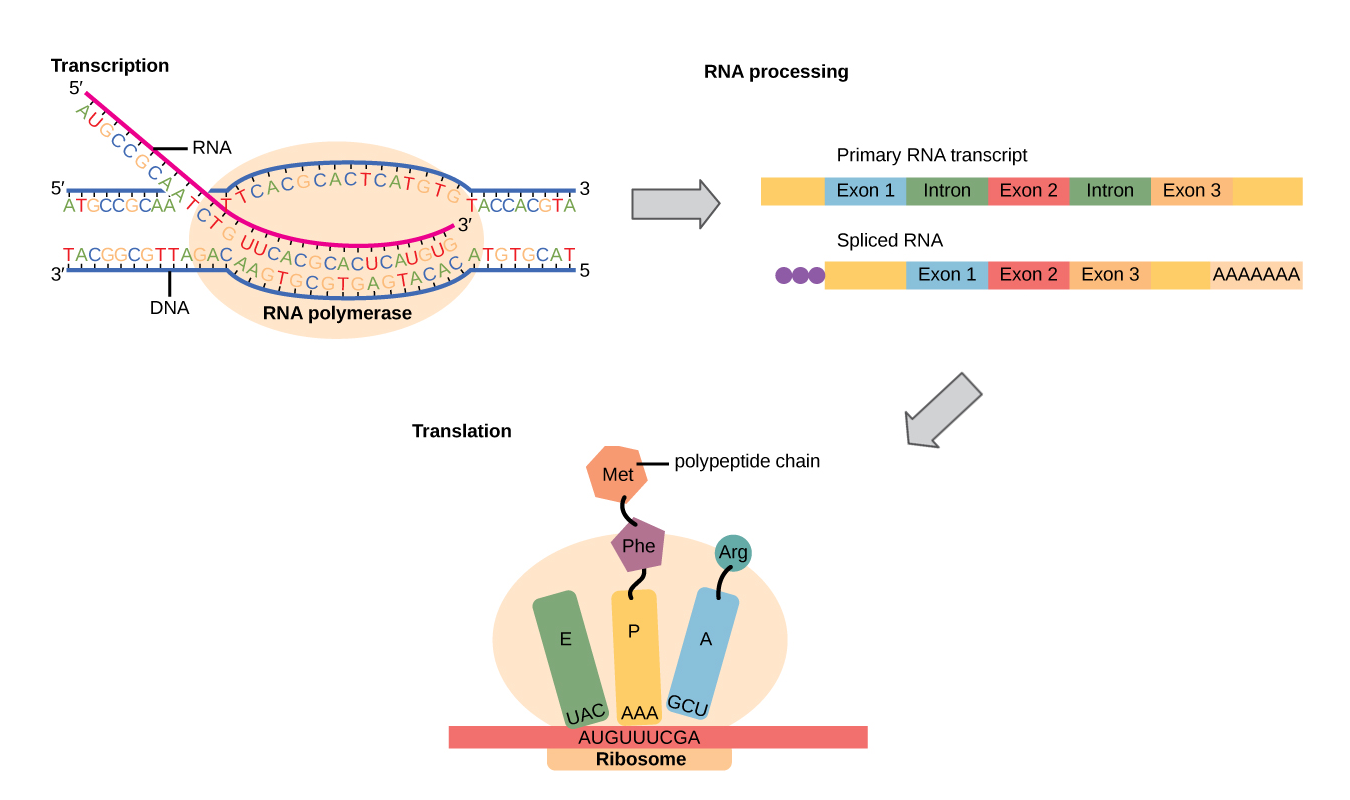
\includegraphics[width=\textwidth]{documents/latex/figures/1/dogma.png}
    \caption{Transferencia de la información genética. El ADN es transcripto en forma de ARN (ARN mensajero). Luego el ARN mensajero es ensamblado uniendo los exones (partes codificantes del gen) en un proceso denominado \textit{splicing}. Por último, los ribosomas usan la información del ARN mensajero para unir los aminoácidos en forma de proteína. Imagen tomada de OpenStax \cite{OpenStaxCNX}.}
    \label{fig:esquema_dogma}
\end{figure}

\begin{figure}[H]
\centering
    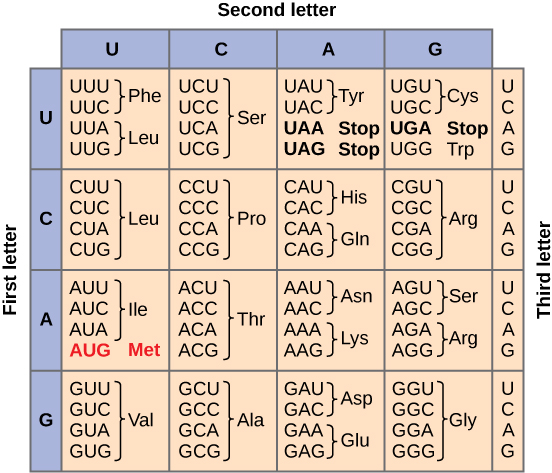
\includegraphics[scale=0.8]{documents/latex/figures/1/tableCodon.jpg}
    \caption{Tabla de codones para generar un determinado aminoácido o símbolo de terminación (\textit{Stop}). Imagen tomada de OpenStax \cite{OpenStaxCNX}.}
    \label{fig:table_codon}
\end{figure}

\newpage

\subsection{Variaciones genéticas}

Las variaciones genéticas son diferencias en el ADN entre individuos de una población \cite{EMBL}. Estas variaciones pueden ser causadas por mutaciones en el momento de la replicación del material genético, pudiendo ser de carácter permanente. Las mutaciones genéticas suelen representar un porcentaje muy pequeño con respecto a la secuencia completa del genoma (alrededor del 0.5\%), pero muchas de ellas suelen ser responsables de variaciones fenotípicas, es decir, nuestros rasgos ``observables''. 

Estas variaciones se pueden dividir en tres grupos principales:

\begin{itemize}
    \item Polimorfismos de un sólo nucleótido (SNPs): sustitución de un único par de bases. 
    \item Inserciones o deleciones (indels): pueden ocurrir en un intervalo grande del ADN de entre 2 a 200 pares de bases.
    
    \item Variaciones estructurales: ocurren en secuencias largas de bases, y pueden ser indels, inversiones, duplicaciones, entre otras.
    
\end{itemize}

Finalmente, cualquiera de estas variaciones pueden ser beneficiosas para el organismo, neutrales (sin efecto alguno) o perjudiciales. 

\subsection{Polimorfismos de un sólo nucleótido (SNPs)}

En el marco de esta tesis estudiaremos los polimorfismos de un sólo nucleótido, o SNPs por sus siglas en inglés (Single Nucleotide Polymorphism). Una persona posee en promedio alrededor de 4 a 5 millones de SNPs. Mientras la mayoría de ellos no tiene efecto en su desarrollo, algunos de ellos pueden variar la respuesta a ciertas drogas, o el riesgo de sufrir algunas enfermedades.

En la figura \ref{fig:snp_types} podemos ver los distintos tipos de SNP. De acuerdo al lugar, pueden ocurrir en una zona codificante, es decir una porción del gen que codifica una proteína, o en una zona no codificante, como los intrones (partes del gen no codificante).

Dentro de las sustituciones en la zona codificante, algunas mutaciones pueden ser sinónimas, es decir que existe un cambio en uno de los nucleótidos del ADN pero no genera un cambio en el aminoácido que codifica. Podemos ver en la tabla \ref{fig:table_codon} que muchos codones codifican el mismo aminoácido, por ejemplo, los codones AUU, AUC y AUA codifican el aminoácido isoleucina. Luego, si en la cadena de ADN, el codón AUA sufre una mutación en su último nucleótido, pasando a ser AUC, dicho codón seguirá codificando para el mismo aminoácido. Otro tipo de sustituciones, denominadas mutaciones sin sentido (\textit{nonsense}) codifican un codón de terminación (\textit{stop}), que resulta en un fin de codificación prematuro y en general una proteína no funcional.

En particular estudiaremos los SNPs con cambio de sentido (\textit{missense}), es decir aquellos que deriven en un cambio de aminoácido en la proteína producida por la variante del gen. 

\begin{figure}[H]
\centering
    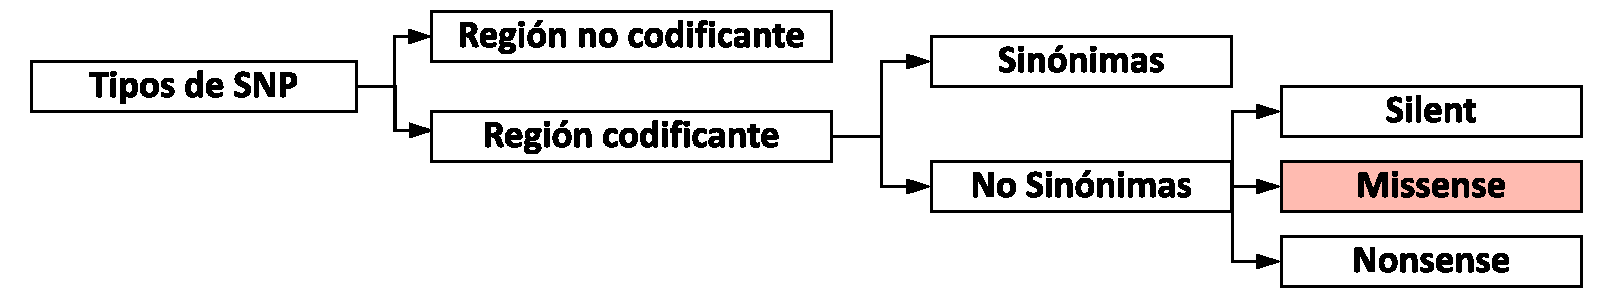
\includegraphics[scale=0.7]{documents/latex/figures/1/snp_types.pdf}
    \caption{Diferentes tipos de SNP de acuerdo a su posición en el genoma y su efecto. En este trabajo nos concentraremos únicamente en las sustituciones \textit{missense}. }
    \label{fig:snp_types}
\end{figure}

\subsection{Bases de datos ómicas}

En la actualidad existen diferentes bases de datos públicas (dbSNP, SNPedia, HapMap, entre otras) que registran millones de estos SNPs \textit{missense}. Los costos de una secuenciación completa siguen bajando de forma acelerada desde el Proyecto Genoma Humano \cite{sequencingcost} (ver figura \ref{fig:cost_per_genome}). Esto ha permitido generar un número creciente de estudios que permiten asociar polimorfismos genéticos a enfermedades (ver figura \ref{fig:dbsnp_growth_rate}). Diferentes bases, como Humsavar \cite{humsavar} o Clinvar \cite{clinvar}, contienen reportes curados con dichos resultados, que se actualizan periódicamente y pueden variar con nueva evidencia. Sin embargo, todavía existe un gran número de SNPs \textit{missense} de los cuales se desconoce su efecto en el organismo. 

% Side by side figures 
\begin{figure}[H]
\begin{minipage}[c]{0.45\linewidth}
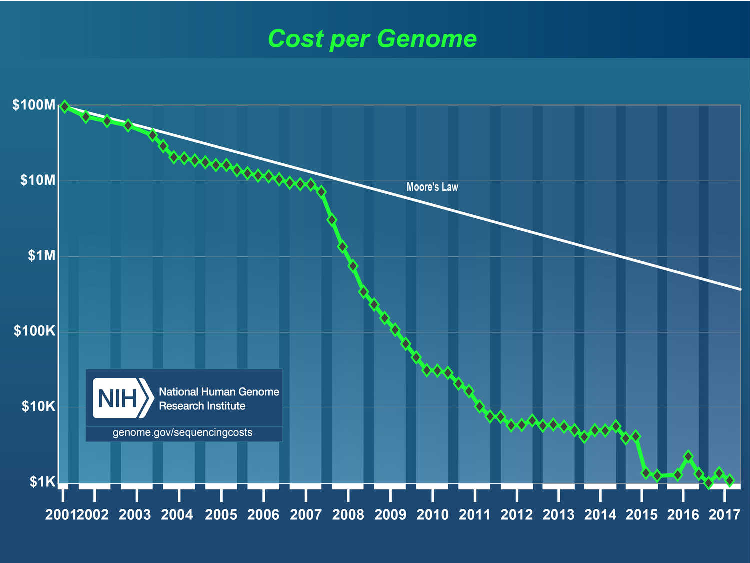
\includegraphics[width=\linewidth]{documents/latex/figures/1/costpergenome_2017.pdf}
\caption{Costo por secuenciación del genoma, NCBI-NIH, 2017. La curva verde corresponde al costo en dólares y la curva blanca equivale a la curva de la ley de Moore, es decir, si se reduciera a la mitad cada año.}
\label{fig:cost_per_genome}
\end{minipage}
\hfill
\begin{minipage}[c]{0.45\linewidth}
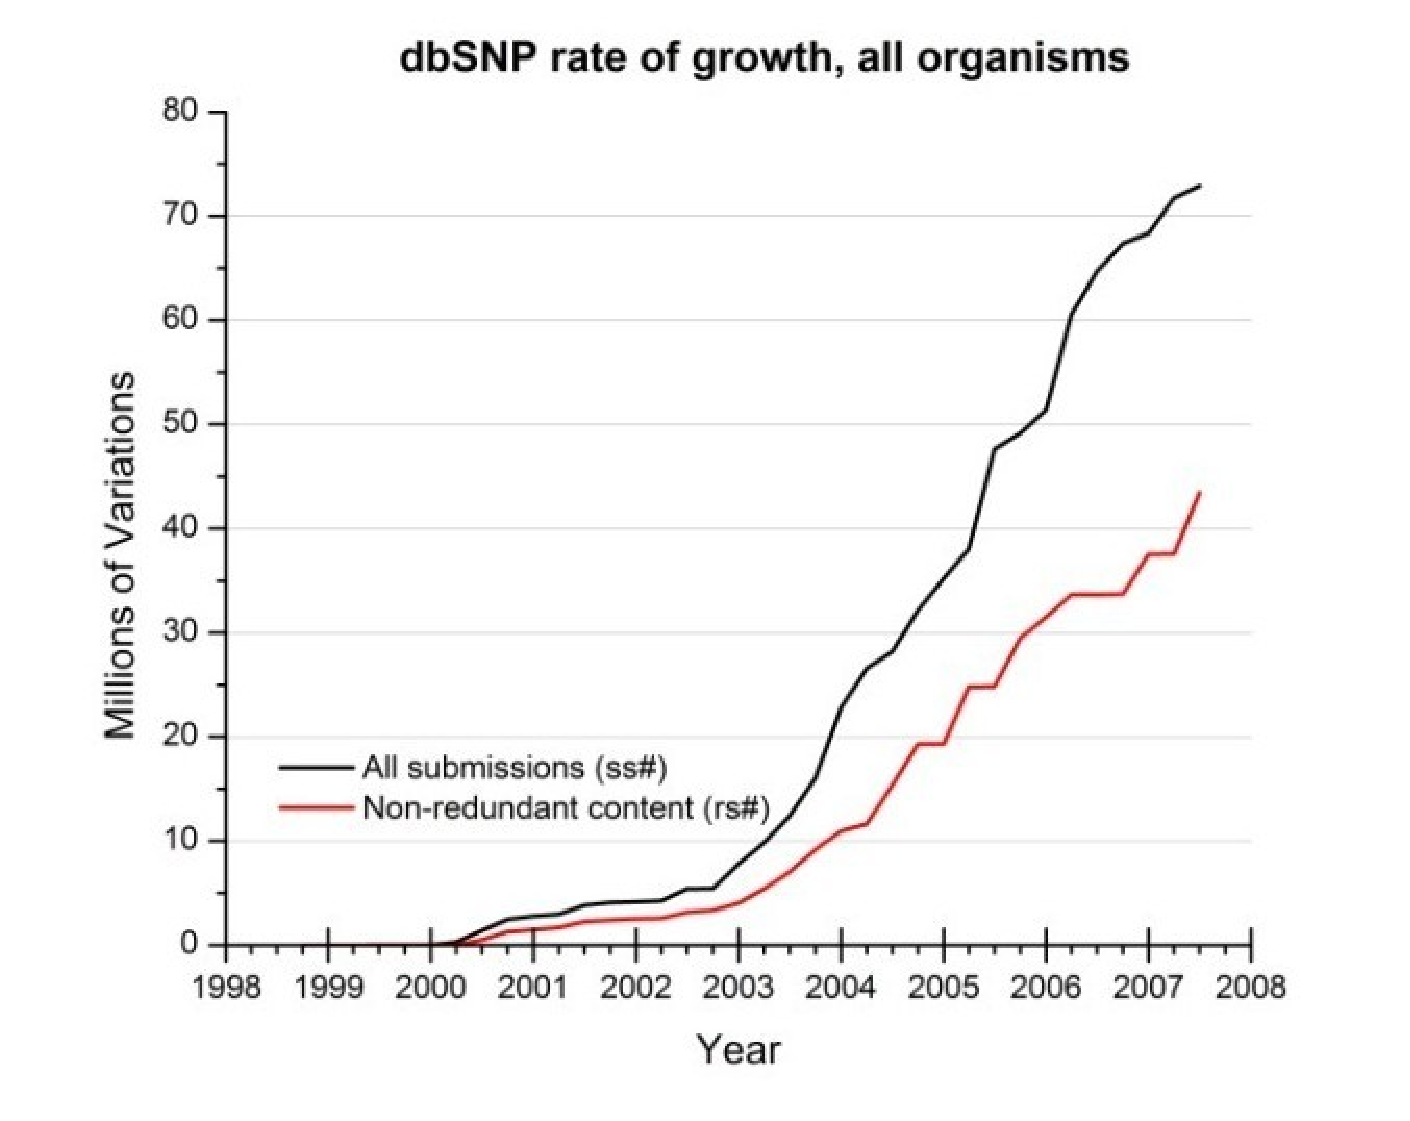
\includegraphics[width=\linewidth]{documents/latex/figures/1/increase_dbsnp.pdf}
\caption{Crecimiento de la base dbSNP a partir del Proyecto Genoma Humano, NCBI-NIH, 2008. La curva negra corresponde a todos los SNPs subidos a la base y la curva roja a los clusters de SNPs que referencian a la misma posición del genoma.}
\label{fig:dbsnp_growth_rate}
\end{minipage}%
\end{figure}

\textbf{El problema biológico que intentaremos atacar es poder predecir aquellos SNPs missense no investigados aún cuyo cambio en el aminoácido de la proteína generada pueda estar asociado a alguna patogénesis}. 

\section{Enfoque computacional}

Para abordar este problema, decidimos usar métodos de aprendizaje automático. El aprendizaje automático es un método computacional (dentro del área de la inteligencia artificial y la estadística) que consiste en aprender a partir de los datos. 

Existen diferentes formas de categorizar los algoritmos de aprendizaje automático. De acuerdo a Barber \cite{Barber2011}, una de las formas posibles es la categorización de acuerdo a la cantidad de tipo de supervisión durante la fase de entrenamiento. Este aprendizaje puede ser:

\begin{itemize}
\item Supervisado, en donde se utilizan ejemplos previos que están ``rotulados'', es decir que poseen una variable de respuesta conocida y se busca conseguir una predicción lo más certera posible sobre nuevos datos. Esta variable de respuesta puede ser continua (problema de regresión) o dividida en clases (problema de clasificación). 
\item No supervisado, donde el objetivo es encontrar distintos grupos o clusters dentro de los datos.
\item Semi-supervisado, en el que se trabaja con un pequeño conjunto de datos etiquetados y un conjunto mucho mayor de datos no etiquetados. El objetivo está en usar este último conjunto para mejorar el clasificador construido con los datos etiquetados.
\item Por refuerzo, donde un \textit{agente} observa el entorno y realiza diferentes acciones para maximizar la recompensa. El modelo a aprender entonces es la estrategia que le permite tomar decisiones ante determinadas situaciones. 
\end{itemize}

Durante la fase de entrenamiento estos algoritmos ajustan sus parámetros de acuerdo a los datos recibidos. En la mayoría de los casos estos algoritmos también poseen hiperparámetros, que no se modifican durante la fase de entrenamiento y determinan algunas de sus características. Estos hiperparámetros pueden ser optimizados mediante técnicas de validación cruzada (ver sección \ref{pipeline}). 

La creciente producción de trabajos nos aporta una gran cantidad de efectos conocidos de las variantes proteicas, y a su vez la ubicación (\textit{locus}) del SNP \textit{missense} responsable en el genoma. Estos datos se encuentran (en gran parte) de forma abierta y gratuita, lo que nos permite aplicar este enfoque computacional. Usando esta fuente de datos entrenaremos un modelo (de forma supervisada) que pueda predecir con un cierto grado de precisión el efecto de una variante aún no reportada. 

% \newpage

\subsection{Aprendizaje supervisado}

Como mencionamos anteriormente, el aprendizaje supervisado trata de predecir una respuesta usando un modelo generado con datos correctamente etiquetados. Definido de manera formal, dado un set de datos $ \mathcal{D} = \{(x^n, y^n), n = 1...N\}$  buscamos aprender la relación entre el ejemplo $x$ y la variable de respuesta $y$ tal que al recibir un nuevo ejemplo $x^*$ la respuesta predicha $y^*$ sea precisa \cite{Barber2011}. La precisión está definida formalmente por la función de pérdida o \textit{Loss Function}, $L(y^{pred}, y^{true})$. Esta función nos permite medir el costo de errar en la predicción y por lo tanto entrenar nuestro modelo de manera que el valor de la función de pérdida usando los datos de entrenamiento sea mínimo o cercano al mínimo.

En el contexto de nuestro problema, cada vector $x$ del set de datos $\mathcal{D}$ es un conjunto de variables que describen a distintos niveles (estructural, físico-químico, genómico) al SNP y a su variante proteica producida e $y$ es el efecto producido en el organismo, basándonos en reportes de Humsavar y Clinvar. Al ser una variable de tipo binaria, podemos aplicar algoritmos de clasificación para este problema.

A continuación haremos un recorrido por los distintos métodos de clasificación que utilizaremos en esta tesis. Estos métodos se encuentran implementados en el módulo \texttt{scikit-learn} de Python \cite{scikit-learn}, excepto por el método Gradient Boosting y su implementación XGBoost \cite{xgboost}. En cada uno de los apartados mencionaremos su funcionamiento general, sus parámetros y sus hiperparámetros. Para estos últimos mencionaremos entre paréntesis su nombre usado en la implementación.

\subsubsection{Regresión logística}

La regresión logística (LR) es un modelo basado en la regresión lineal. Al igual que ésta, consiste en buscar los coeficientes de una función de manera que el valor de la función de pérdida sea el mínimo. A diferencia de la regresión lineal, que usa una función lineal (o polinomial) para aproximar los puntos (que son valores continuos), la regresión logística usa la función logística para aproximar los valores (que son categóricos). Esta función, generalizada para múltiples variables predictoras y variable de respuesta binaria se define como:

\begin{equation*}
h_{\theta}(\boldsymbol{X}) = \frac{1}{1 + e^{\theta^{T}\boldsymbol{X}}} = Pr(Y = 1 | \boldsymbol{X}; \theta)
\end{equation*}

donde $\boldsymbol{X}$ representa el vector de variables predictoras, $\theta$ es el vector de coeficientes ($\theta^{T}$ representa al vector transpuesto) e $Y$ es la variable de respuesta \cite{Barber2011}. Lo que se busca modelar, es la probabilidad de pertenecer a una clase determinada (simbolizada con '1'), cuando las variables observadas son $\boldsymbol{X}$ y usando los parámetros $\theta$. La probabilidad de pertenecer a la otra clase entonces, es igual a 1 - $h_{\theta}(\boldsymbol{X})$. 

Los parámetros $\theta$ son obtenidos buscando maximizar la verosimilitud con los parámetros de la distribución real de los datos \cite{Hastie2001}, mientras que los hiperparámetros ($\Tilde{\theta}$) se obtienen usando validación cruzada (ver sección \ref{pipeline}). Los hiperparámetros que buscaremos optimizar son dos:

\begin{itemize}
    \item El parámetro de regularización (\texttt{C}): Parámetro usado para penalizar el uso de muchas variables en la función de pérdida, simplificando el modelo y previniendo un posible \textit{overfitting}.
    \item El balance de las clases (\texttt{class\_weight}): Pesos asociados a la importancia a la que se le da reconocer una determinada clase, penalizando el error en la función de pérdida con un valor asignado en lugar de 1. 
\end{itemize}

\subsubsection{Support Vector Machines}

Las Support Vector Machines (SVM) se desarrollaron inicialmente como métodos lineales de clasificación, al igual que la regresión logística. Esto significa que también buscan una frontera de decisión (\textit{decision boundary}) que define la clase a la que pertenecen los datos usando una combinación lineal de las variables predictoras. En este caso no se busca hallar los parámetros de la distribución a modelar sino que el objetivo reside en encontrar el hiperplano (\textit{Support Vector}) que mejor separe a los datos de entrenamiento \cite{Hastie2001}. Posteriormente este método fue extendido para buscar un hiperplano en un espacio de variables transformado (método no lineal). Esta transformación se logra reemplazando el producto interno por una función kernel. En este trabajo haremos uso de la función de base radial (RBF, por sus siglas en inglés), que es la más comúnmente usada en este método. En este algoritmo buscaremos optimizar dos hiperparámetros: 

\begin{itemize}
    \item El parámetro de penalidad (\texttt{C}): Este parámetro regula que tan bien debe el hiperplano separar las clases a costa de una distancia menor en la frontera de decisión. Es decir, un valor elevado de \texttt{C} se ajustará mejor a los datos de entrenamiento, mientras que un valor bajo será más general, a costa de errores.
    \item Gamma (\texttt{gamma}): Define que tan lejos alcanza la influencia de cada uno de los ejemplos de entrenamiento en la creación de la frontera de decisión.  
\end{itemize}  

\subsubsection{Random Forest}

A diferencia de los algoritmos anteriores, Random Forest (RF) esta basado en un método de clasificación basado en árboles de decisión. Estos métodos se caracterizan por segmentar el espacio de predicción en un número de regiones. Para entender Random Forest, resulta muy útil conocer el funcionamiento de éstos árboles. 

Un árbol de decisión se construye dividiendo el espacio de variables de forma recursiva, recorriendo la lista de variables y seleccionando la variable que mejor divide las clases de acuerdo a un criterio determinado. El criterio que decidimos usar en este trabajo, por ser el más usado en tareas de clasificación, es el índice Gini (también referido como pureza):

\begin{equation*}
    G = \sum_{k = 1}^{K} \hat{p}_{mk}(1 - \hat{p}_{mk})
\end{equation*}

donde $\hat{p}_{mk}$ representa la proporción de la clase $k$ en la región $m$ \cite{Hastie2001}. Uno de los principales problemas que presenta este enfoque es la alta varianza (\textit{variance}) con respecto a los datos de entrenamiento. Si la profundidad del árbol es muy grande, aumenta el riesgo de \textit{overfitting} en los datos que poseemos. 

En el caso de Random Forest, se construyen distintos árboles de decisión con subconjuntos de variables escogidos de forma aleatoria, con el objetivo de disminuir la varianza. A la vez, al ser árboles de poca profundidad (que favorecen el \textit{underfitting}), se genera una cantidad alta de árboles para solucionar el problema de alto sesgo (\textit{bias}). 

Esta técnica consistente en combinar distintos algoritmos para obtener un mejor predictor se la denomina \textit{ensamble}, y en particular, Random Forest se enmarca dentro de la técnica de \textit{bagging}. Esto significa que la predicción final se obtiene a través de un promedio de los predictores que componen el método con igual peso.

Una de las principales ventajas de Random Forest es su interpretabilidad. Esto se expresa en la posibilidad de calcular fácilmente la importancia de las variables en el modelo. La importancia de una variable (o \textit{feature importance}) se calcula como el promedio del índice Gini en cada uno de los nodos de los árboles donde aparece, expresada proporcionalmente a la importancia máxima de todas las variables \cite{Hastie2001}.
Finalmente, el algoritmos posee una serie de hiperparámetros a ser tuneados. Nosotros buscaremos optimizar los siguientes:

\begin{itemize}
    \item Profundidad del árbol (\texttt{max\_depth}): La profundidad máxima de cada árbol.
    \item Estimadores (\texttt{n\_estimators}): La cantidad de árboles.
    \item Cantidad de variables por árbol (\texttt{max\_features}): En cada split del árbol, se puede fijar la cantidad de variables a comparar.
\end{itemize}

\subsubsection{Gradient Boosting y XGBoost}

Gradient Boosting (GB) es otro método de ensamble, que como las otras técnicas de \textit{boosting}, genera modelos de forma iterativa, modificando el algoritmo para intentar corregir los errores de la iteración anterior. Esta es una diferencia crucial con respecto a los algoritmos de \textit{bagging}, como Random Forest, que genera modelos de forma paralela. La forma en que Gradient Boosting busca mejorar iterativamente es modelando el vector residual (o en otras palabras, la distancia entre la predicción y la variable a predecir) generando de esta manera un modelo aditivo que se puede representar de la siguiente manera:

\begin{equation*}
    F_{m}(X) = F_{m - 1}(X) + \eta \cdot \Delta_{m}(X) 
\end{equation*}

donde $F_{m - 1}(X)$ es el modelo del paso anterior, $\Delta_{m}(X)$ es el modelo del vector residual y $\eta$ es el \textit{learning rate}, un hiperparámetro que busca regularizar la importancia de este factor en el modelo final para reducir el \textit{overfitting} \cite{gradient}. 

En este trabajo vamos a utilizar XGBoost (XGB), una implementación de Gradient Boosting con árboles muy utilizado en competencias Kaggle \cite{xgboost}. Este algoritmo cuenta con una gran cantidad de hiperparámetros, al ser un método de ensamble combina los hiperparámetros de los \textit{tree boosters} con los pertenecientes al método Gradient Boosting. Decidimos limitarnos a un número relativamente pequeño de hiperparámetros buscando referencias de su uso, aunque dejamos la exploración de los restantes para un trabajo futuro. Los hiperparámetros explorados fueron:

\begin{itemize}
    \item Peso mínimo de las hojas (\texttt{min\_child\_weight}): Mínima suma del peso de las instancias (hessiano) necesaria en un hoja para dejar de realizar cortes.
    \item Gamma (\texttt{gamma}): Mínima pérdida requerida para la creación de un nuevo corte en el árbol.
    \item Muestreo (\texttt{subsample}): Proporción de muestra de los ejemplos antes de la construcción del árbol. 
    \item Cantidad de variables por árbol (\texttt{colsample\_bytree}): Mismo parámetro que en Random Forest.
    \item Profundidad máxima (\texttt{max\_depth}): Mismo parámetro que en Random Forest.
\end{itemize}

\subsection{Pipeline de entrenamiento, validación y evaluación} \label{pipeline}

Cada uno de estos métodos involucran una fase de entrenamiento, validación y evaluación. En la fase de entrenamiento los algoritmos ajustan sus datos de acuerdo a sus distintas funciones de pérdida. En nuestro trabajo también buscamos aproximarnos al mejor set de valores de hiperparámetros usando una técnica llamada \textit{Grid-Search}. Este método consiste en evaluar distintos valores para cada parámetro, que en conjunto forman una grilla (o \textit{grid}). 

Para cada conjunto de hiperparámetros de esta grilla se entrena el modelo y finalmente se elige el conjunto de hiperparámetros que haya tenido mejor performance (bajo alguna métrica, ver sección \ref{eval_metrics}). Al evaluar la performance de cada conjunto de hiperparámetros no podemos volver a usar el mismo conjunto de datos para el que fue entrenado, por lo que para evitar esto usamos otra técnica llamada \textit{k-fold Cross Validation}. La idea es generar un corte (\textit{split}) en el dataset de entrenamiento con el objetivo de poder evaluar los hiperparámetros en un conjunto de datos que no haya sido utilizado (conjunto de validación). Este procedimiento se realiza $k$ veces con diferentes splits realizados al azar, con una proporción igual en cada subconjunto o \textit{fold}. Una vez elegido el modelo entrenado con el mejor conjunto de hiperparámetros se evalúa en un dataset de evaluación (que no fue usado durante el entremiento) de acuerdo a las métricas de la sección \ref{eval_metrics}.

% \newpage

\subsection{Métricas de evaluación} \label{eval_metrics}

Las medidas que utilizaremos para evaluar la performance del modelo son las siguientes:

\begin{itemize}

    \item \textbf{Precisión}: La Precisión del modelo, está medida como la cantidad de positivos correctamente clasificados (VP) sobre la cantidad de instancias clasificadas como positivas: verdaderos positivos (VP) y falsos positivos (FP).
    
    \begin{equation*}
        \frac{VP}{VP + FP}
    \end{equation*}
    
% \pagebreak
    \item \textbf{Recall}: El Recall corresponde a la cantidad de verdaderos positivos sobre el total de positivos: verdaderos positivos (VP) y falsos negativos (FN).
    
    \begin{equation*}
        \frac{VP}{VP + FN}
    \end{equation*}
    
    \item \textbf{F1-Score}: El F1-Score es el promedio armónico entre la Precisión y el Recall. Usamos el promedio armónico de manera de afectar negativamente el resultado si alguno de los valores es especialmente bajo. Posee un rango de 0 a 1. 
    
    \begin{equation*}
        F_1 = \frac{2}{\tfrac{1}{\mathrm{recall}} + \tfrac{1}{\mathrm{precision}}} = 2 \cdot \frac{\mathrm{precision} \cdot \mathrm{recall}}{\mathrm{precision} + \mathrm{recall}}
    \end{equation*}
    
    % \newpage
    
    \item \textbf{Área bajo la curva ROC (AUC)}: La curva ROC está generada por dos métricas principales, FPR y TPR:
    
    \begin{multicols}{2}
        \begin{equation*}
        TPR = \frac{VP}{VP + FN}
        \end{equation*}
        \break
        \begin{equation*}
        FPR = \frac{FP}{FP + VN} 
        \end{equation*}
    \end{multicols}
    
    En un contexto de clasificación binaria, si ordenamos al score de predicción final de mayor a menor y consideramos positivos a todos aquellos a la izquierda del umbral de decisión (\textit{threshold}), obtendremos una tasa de verdaderos positivos y de falsos positivos (TPR y FPR respectivamente). Esto puede verse en la figura \ref{fig:threshold_auc}.
    
    \begin{figure}[H]
    \centering
        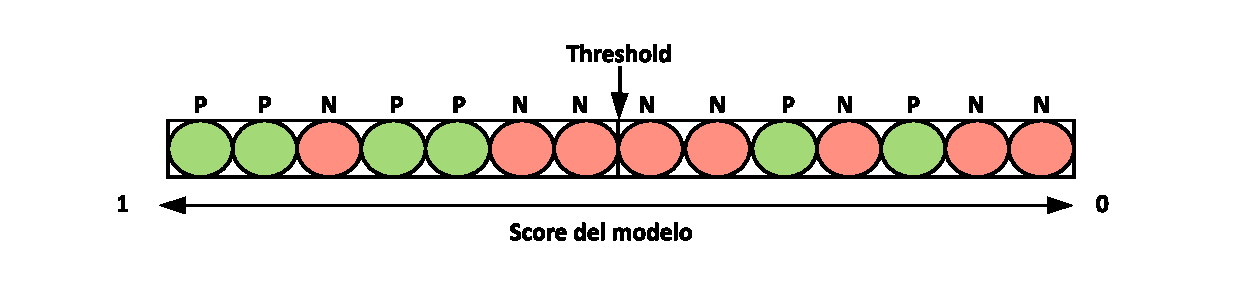
\includegraphics[scale=0.6]{documents/latex/figures/1/threshold_auc.pdf}
    \caption{Predicciones ordenadas de mayor a menor, donde el \textit{threshold} asigna clasificación positiva y negativa. El color de las instancias indica el valor real. En este caso el $TPR$ es igual a 2/3 y el FPR es igual a $3/8$.}
    \label{fig:threshold_auc}
    \end{figure}
    
    La curva característica operativa del receptor (ROC, por sus siglas en inglés) es la representación gráfica de la relación entre el FPR y el TPR al mover el umbral de decisión. 

    En la figura \ref{fig:example_roc} puede verse la curva que representa el ejemplo de la figura \ref{fig:threshold_auc}.
    
    \begin{figure}[H]
        \centering
        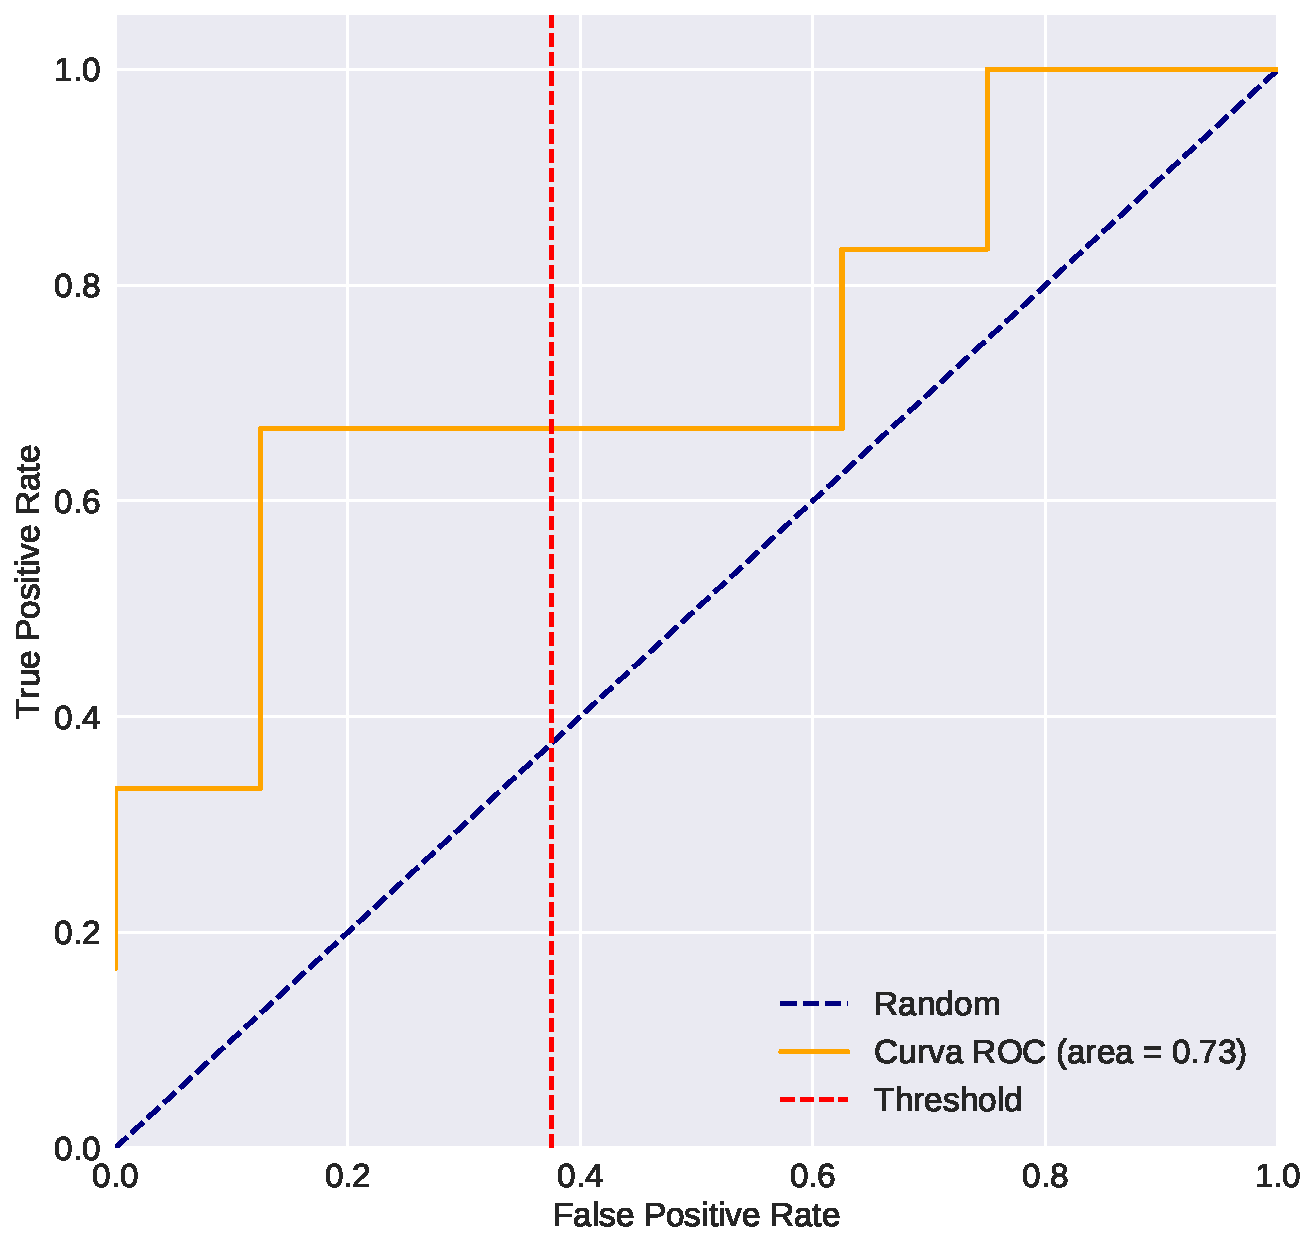
\includegraphics[scale=0.4]{documents/latex/figures/1/roc_ejemplo.pdf}
        \caption{Curva ROC de la clasificación de la figura \ref{fig:threshold_auc}. La línea punteada roja representa el umbral de decisión, que fijó el FPR y TPR en los valores anteriormente mencionados.}
        \label{fig:example_roc}
    \end{figure}
    
    Su área (AUC, por sus siglas en inglés) equivale a la probabilidad de que el modelo clasifique una instancia positiva cualquiera ``mejor'' que una instancia negativa cualquiera (estadístico Mann-Whitney $U$ \cite{doi:10.1256/003590002320603584}). Dadas dos muestras de tamaño $n_1$ y $n_2$, el estadístico Mann-Whitney $U$ se define como:
    
    \begin{equation*}
        U = \sum_{i = 1}^{n_1} r_{1i} - \frac{n_1 (n_1 + 1)}{2}
    \end{equation*}
    
    donde $r_{1i}$ es el ranking del elemento $i$ de la muestra $n_1$. La equivalencia con este estadístico viene de considerar a los verdaderos positivos y falsos positivos como muestras $n_1$ y $n_2$ respectivamente. Su distribución es aproximadamente normal para muestras grandes \cite{mann1947}, lo que nos permite calcular su intervalo de confianza. Otro método, el test de DeLong, utiliza este mismo concepto para evaluar y comparar curvas de AUC \cite{DeLong}.

\end{itemize}

% \newpage


\section{Trabajos relacionados}

A partir de mutaciones conocidas y sus propiedades asociadas, deseamos explorar un método de aprendizaje automático supervisado que nos permitan generar un modelo que, ante una mutación no estudiada, pueda predecir su patogenicidad. Para recolectar datos, asociados a mutaciones conocidas, existen múltiples herramientas. En particular, para el presente trabajo vamos a explorar: VarQ, VEST y FATHMM-MKL.

\subsubsection{VarQ}

VarQ es una herramienta generada en la BIA (Plataforma Bioinformática Argentina) por Leandro Radusky \cite{Radusky2017}. Esta herramienta permite extraer datos estructurales de variantes proteicas de un sólo aminoácido (SAS, por sus siglas en inglés) tomando información de diferentes bases de datos o aplicaciones (PDB, PFam, 3DID, entre otras), permitiendo el análisis manual de los diferentes cambios estructurales, como el tipo de actividad, el plegamiento, si pertenece a un sitio activo, o si forma parte en interfaces proteína-proteína, como se ve en la figura \ref{fig:varq_pipeline}. 

\begin{figure}[H]
    \centering
    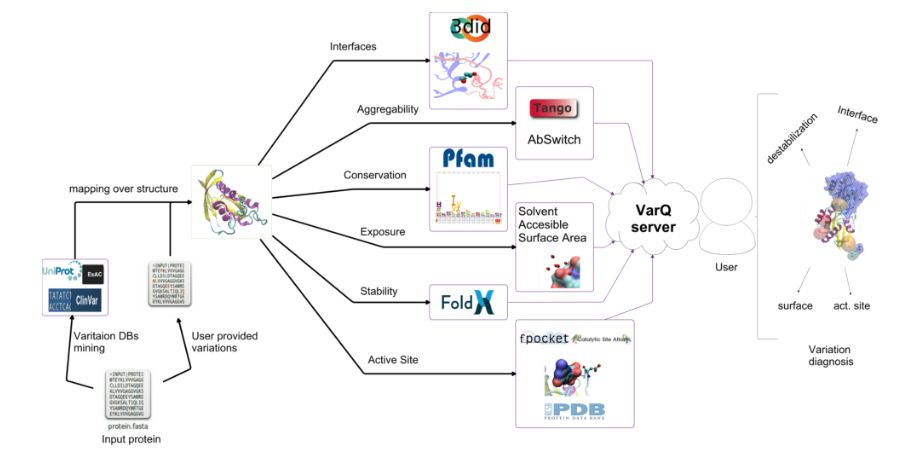
\includegraphics[scale=0.45]{documents/latex/figures/1/pipeline.png}
    \caption{Pipeline de extracción de datos de la herramienta VarQ. Esta figura fue extraída de la tesis de doctorado de Leandro Radusky \cite{Radusky2017}.}
    \label{fig:varq_pipeline}
\end{figure}

En la primera parte de esta tesis hacemos uso del trabajo de tesis de grado de Santiago Moreno (todavía en elaboración). Uno de sus objetivos principales fue generar un dataset de variantes a nivel de proteínas (al que denominaremos dataset VarQ), y evaluar la performance de un modelo que predice el efecto de la mutación usando las variables que provee esta herramienta. En la capítulo \ref{ch:desarrollo_varq} presentaremos un modelo de clasificación, variando las técnicas de aprendizaje automático presentadas, y creado en base a las variables que provee a este dataset. Posteriormente encontraremos sus limitaciones para tal fin.

\subsubsection{VEST}

VEST (\textit{Variant Effect Scoring Tool}) \cite{Carter2013} es un predictor de efectos funcionales de SNPs \textit{missense} desarrollado en el Karchin Lab de la Universidad de Johns Hopkins. Con esta herramienta (basada en Random Forest) analizaron aproximadamente 80,000 variantes anotadas de HGMD (\textit{Human Gene Mutation Database}) con variables de tipo genómicas, estructurales y físico-químicas usando la base de datos SNVBVox, desarrollado por el mismo equipo. A lo largo de nuestro trabajo integraremos muchas de las variables de esta base de datos a nuestros datasets.

\subsubsection{FATHMM-MKL}

FATHMM-MKL (\textit{Functional Analysis through Hidden Markov Models}) \cite{Shihab2015} es también un predictor de efectos funcionales de SNPs \textit{missense}, en regiones codificantes y no codificantes. El modelo está basado en SVM usando una combinación de múltiples kernels (\textit{Multiple Kernel Learning, MKL}). Fue desarrollado en la Universidad de Bristol. Uno de los puntos interestantes del trabajo es un suplemento con la descripción de las variables usadas. A partir de este informe buscaremos conseguir algunas de las variables usadas que hayan tenido mayor impacto en el modelo.

% \newpage


\section{Objetivos y estructura del trabajo}

El objetivo del trabajo se centra en responder una serie de interrogantes generados a partir del estudio de los trabajos previos:

\begin{itemize}
    \item El dataset de VarQ se compone esencialmente de variables de tipo estructural. ¿Es posible enriquecerlo con variables de otras dimensiones (físico-químicas, genómicas, filogenéticas)?
    \item ¿Cómo afectan las distintas variables a nuestros modelos de predicción de patogenicidad de los SNPs? ¿Cuáles son las más importantes para predecir una variante patogénica?
    \item ¿Cuáles son los mejores algoritmos de aprendizaje automático para resolver este tipo de problemas y cuáles son sus hiperparámetros?
    
\end{itemize}

Estos puntos serán abordados generando y estudiando modelos de aprendizaje automático sobre distintos conjuntos de variables descriptivas para los SNPs, como se describe a continuación:

\begin{itemize}
    \item Modelo usando el dataset VarQ
    \item Modelo usando propiedades físico-químicas de la proteína
    \item Modelo usando variables genómicas
    \item Integración de propiedades físico-químicas y variables genómicas
    \item Integración de propiedades físico-químicas, variables genómicas y las variables del dataset VarQ.
\end{itemize}




\chapter{Modelo basado en el dataset VarQ}
\label{ch:desarrollo_varq}
% \section{Modelo usando el dataset VarQ}

Comenzamos nuestro trabajo analizando el dataset construido en la tesis de Santiago Moreno. Este dataset fue construido inicialmente con las variantes originales del sitio de VarQ \cite{varq}, que consistieron en aproximadamente 400 mutaciones correspondientes a 13 proteínas con 10 variables. Posteriormente en el mismo trabajo se aumentó la cantidad para llegar a las aproximadamente 18 mil variantes del dataset VarQ usando otras fuentes como Clinvar \cite{clinvar} y Humsavar \cite{humsavar}. Llamaremos a este dataset VarQ Completo. 

\section{Variables del dataset VarQ Completo}

A continuación damos una descripción detallada de las variables originales encontradas en el dataset. Presentamos un extracto del trabajo de Santiago Moreno en donde se describen dichas variables: 

\begin{itemize}
    \item Variación de Energía (ENE): En VarQ, las mutaciones son modeladas con el software FoldX \cite{Schymkowitz2005}, que construye un modelo a partir de una estructura dada y luego muta residuos específicos. Luego el software predice el impacto energético de la mutación en la estabilidad de la proteína o, en caso de tratarse de un complejo, en la estabilidad del mismo.
    \item SASA: Es el valor correspondiente a la superficie accesible por parte del solvente, de la cadena lateral del aminoácido. Este valor permite determinar si la cadena lateral se encuentra en la superficie o en el núcleo de la estructura.
    \item Porcentaje de SASA: El porcentaje que representa el SASA sobre el total. Es decir el porcentaje que representa el SASA en función de la estructura de la proteína.
    \item B-Factor (BF): o factor de temperatura, que corresponde a un aminoácido dentro de la proteína. Una mayor temperatura, indica que el aminoácido pertenece a una zona potencialmente de mayor movilidad.
    \item Switchability (SWI): Evalúa cuán propenso a generar un cambio de hélice alfa a hoja beta es un conjunto de aminoácidos \cite{PMID:25082719}.
    \item Aggregability (AGG): El software Tango \cite{Fernandez-Escamilla2004} evalúa cuán
    propenso es un aminoácido a generar agregación en una proteína desde un punto de vista estructural. La agregación es el proceso por el cual proteínas mal formadas
    adoptan una conformación que causa su polimerización en fibrillas agregadas y organizadas. Muchas enfermedades neurodegenerativas, como por ejemplo la Amiloidosis, están asociadas con la agregación proteica.
    \item Conservación (CONS): Se calcula en bits, siempre y cuando la mutación pueda ser mapeada a una posición en una familia PFam asignada \cite{Finn2014}. Cuando una posición tiene un alto valor en bits y la misma posición coincide con el aminoácido conservado en la secuencia de la proteína interpretamos que dicha posición está altamente conservada. La misma puede estar altamente conservada porque es importante estructuralmente o porque es importante para la actividad enzimática \cite{Radusky2017}. Los residuos con alta conservación tendrán un impacto mayor sobre la función pues afectan aminoácidos de la familia.
    \item Sitio Activo (AS): Las posiciones de sitio activo son aquellas que se encuentran marcadas como unidas a ligandos en los archivos PDB o que pertenecen al mismo \textit{pocket} que se encuentren conteniendo estos residuos nombrados o aquellos que pertenezcan al Catalytic Site Atlas \cite{Porter2004}.
    \item Interfaz 3DID: Determina si la posición sirve para una interfaz proteína-proteína según la base de datos de 3DID \cite{Stein2005}.
    \item Interfaz PDB: Determina si la posición sirve para una interfaz proteína-proteína según la base de datos de PDB \cite{Berman2003}.
\end{itemize}


\section{Limpieza del dataset VarQ Completo}

Para trabajar con este dataset decidimos verificar la etiqueta de cada una de las variantes, de manera de confirmar que su status siguiera vigente. Para esto recurrimos a las fuentes Clinvar y Humsavar. Realizamos un primer filtrado de estas tablas quedándonos con aquellas variables con un status confirmado: en el caso de Humsavar, aquellas que figuran con la expresión \textit{Polymorphism} y \textit{Disease}, mientras que en Clinvar nos quedamos con aquellas que figuraban como \textit{Benign} y \textit{Pathogenic}, eliminando aquellas con caracterización difusa, por ejemplo, \textit{Risk Factor} (factor de riesgo). 

\begin{figure}[H]
    \centering
    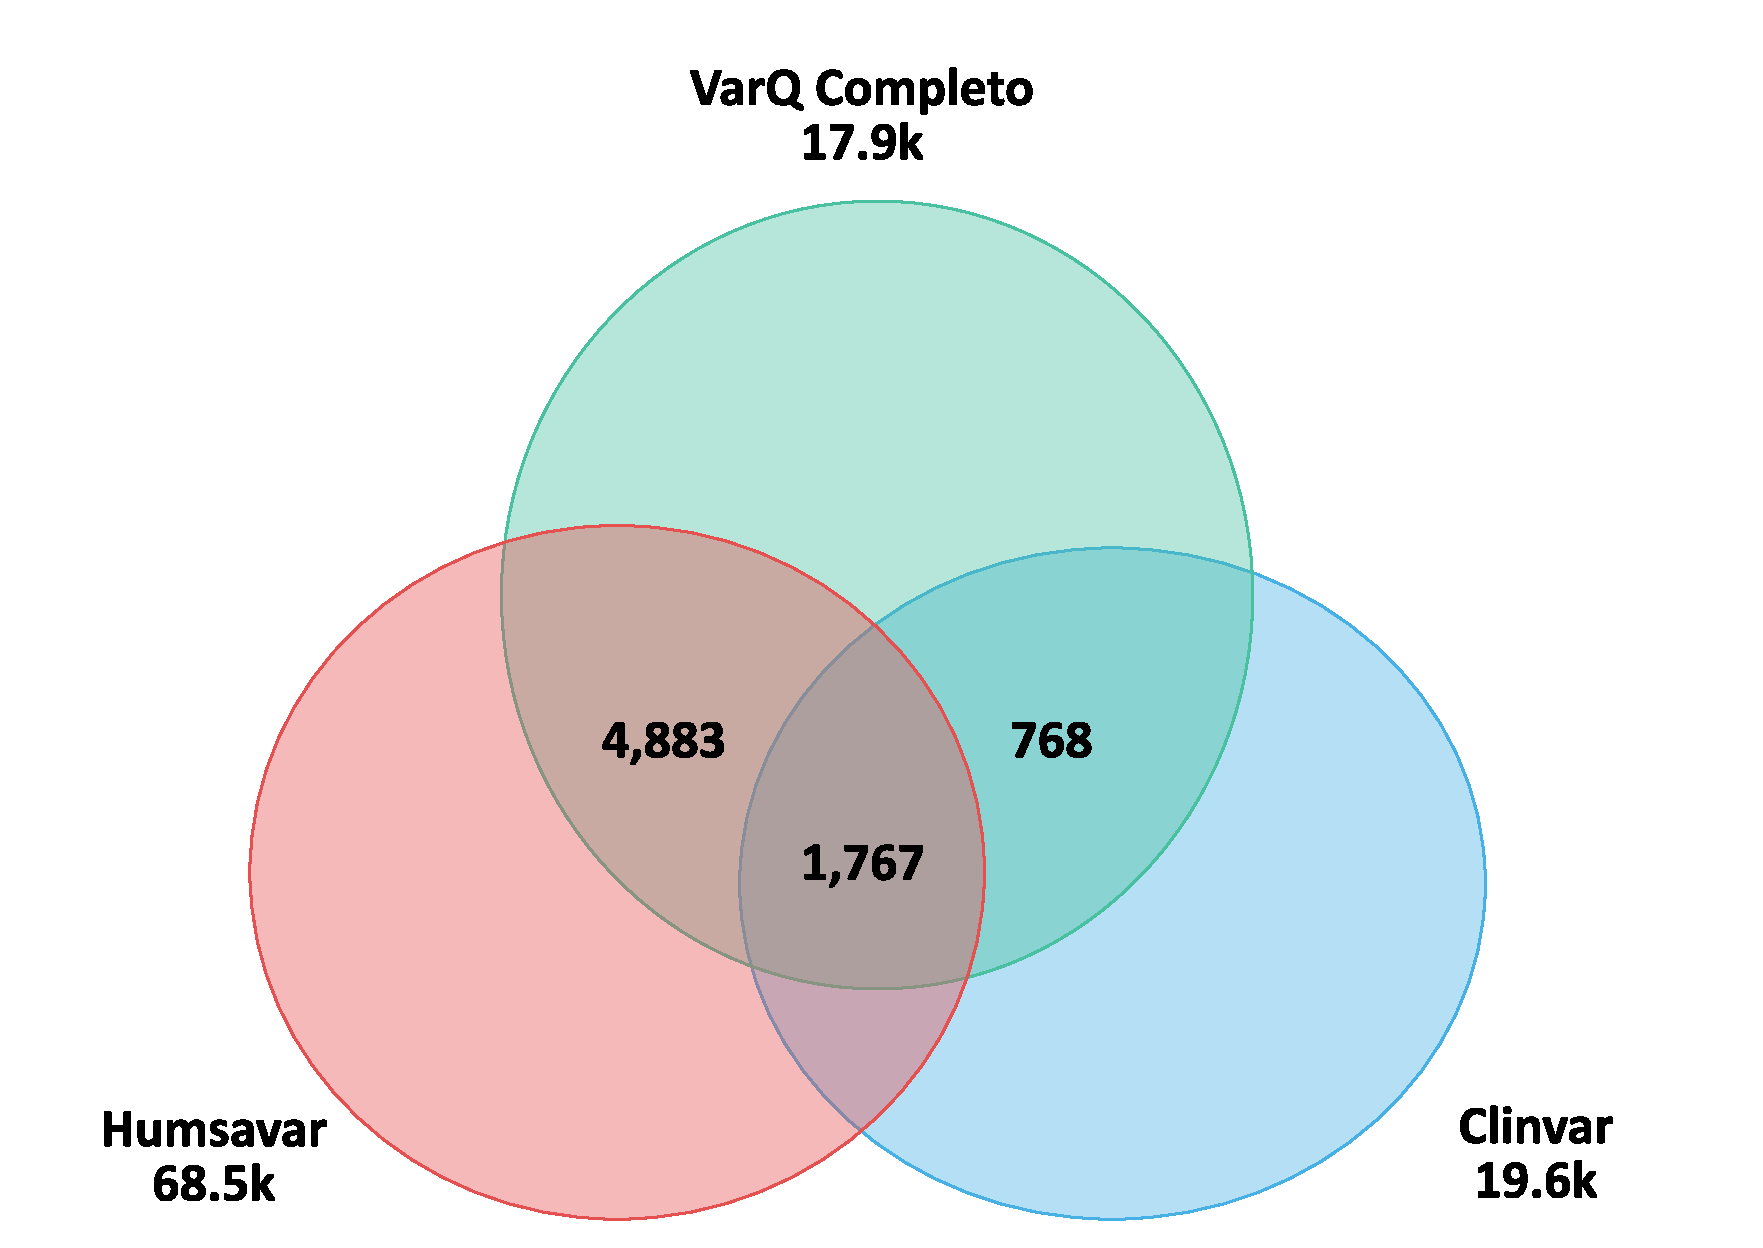
\includegraphics[scale=0.4]{documents/latex/figures/3/varq/interseccion_varq.pdf}
    \caption{Valores en la intersección del dataset VarQ Completo con las tablas Clinvar y Humsavar.}
    \label{fig:interseccion_varq}
\end{figure}

Así, cruzamos los datos con las tablas filtradas Humsavar y Clinvar, y encontramos un subconjunto importante de variantes que no aparecían en ninguna de las dos fuentes. Estas variantes estaban rotuladas en su gran mayoría (94\%) como benignas, por lo que creemos que se consideraron como variantes benignas a todas aquellas a las que no se encontró un reporte. Decidimos remover estas variantes del dataset por considerar que si alguna de ellas estuviera rotulada incorrectamente introduciría ruido. Como puede observarse en la figura \ref{fig:interseccion_varq}, de las 17,869 variantes del dataset VarQ Completo, logramos encontrar 2,535 en la tabla de Clinvar, de los cuales sólo 2,397 tenían un estado confirmado como patogénicas, y 138 como benignas. Cruzando el dataset con la tabla Humsavar encontramos una intersección de 6,650 variantes de los cuales 4,667 corresponden a patogénicas y 1,983 son benignas. Decidimos mantener la clasificación de Humsavar en la intersección de los tres conjuntos por considerarla de mayor confiabilidad dado que es un reporte único curado por expertos, a diferencia de Clinvar que es una recopilación de variantes de diversa significación clínica, y a menudo presenta conflictos de anotación por discrepancias entre evidencias reportadas. Esto nos dejó con un dataset de 7,418 variantes de las cuales 5,377 son patogénicas y 2,041 son benignas. Denominamos a este dataset VarQ Curado. 


\section{Descripción estadística del dataset VarQ Curado}

A partir de VarQ Curado estudiaremos sus variables usando estadísticas descriptivas con el objetivo de evaluar la calidad del dataset. La idea es poder tener una noción de la dispersión de nuestros datos, sumado a la cobertura que tenemos de ellos sobre las variantes.

En la figura \ref{fig:proporcion_nulos_varq} podemos observar cómo la variable de sitio activo (ACTIVE\_SITE) no posee datos para casi ninguna variante (aproximadamente el 95\%), mientras que la variable de conservación (CONS) no posee datos para el 63\% de las variantes. En base a estas observaciones decidimos remover la variable de sitio activo del dataset por considerarla muy poco relevante en términos de cobertura.

\begin{figure}[H]
    \centering
    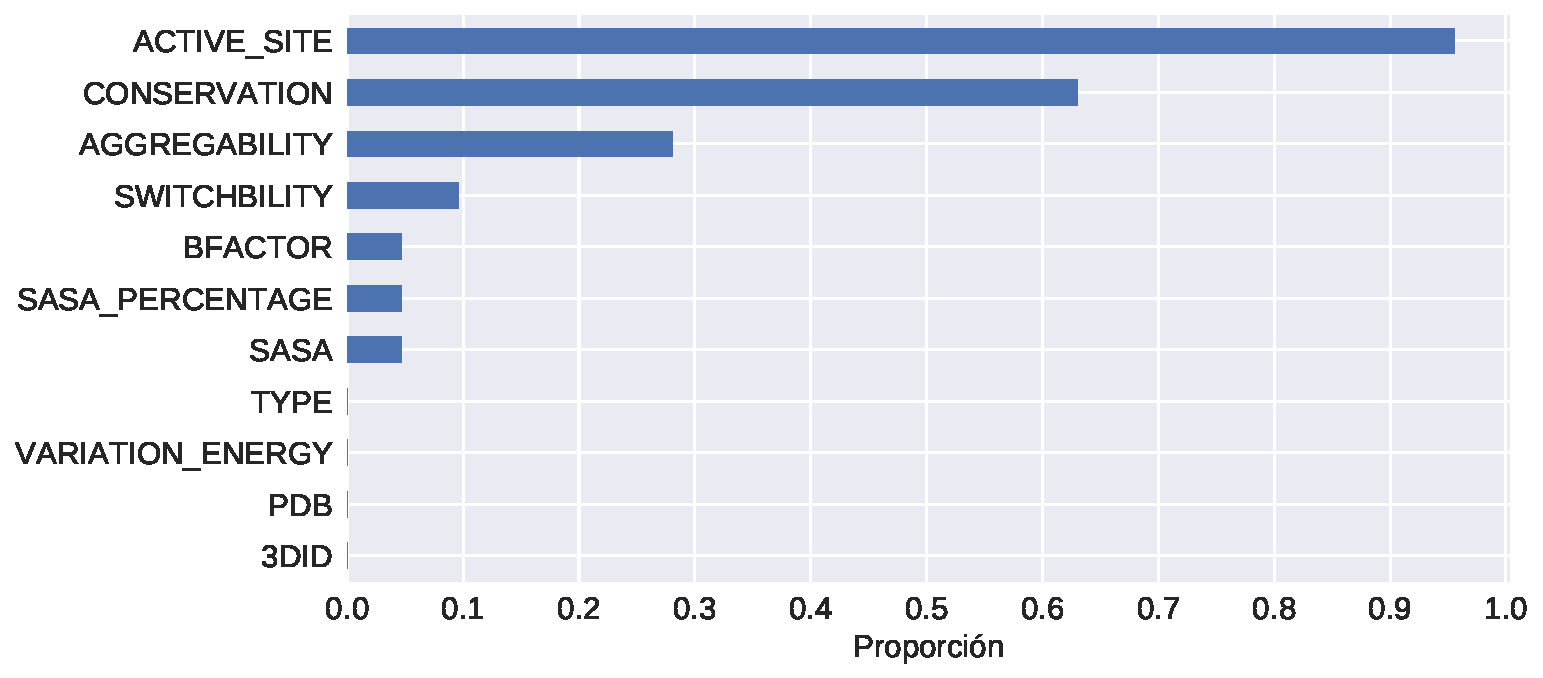
\includegraphics[scale=0.6]{documents/latex/figures/3/varq/proporcion_nulos.pdf}
    \caption{Proporción de variantes con valor nulo por variable del dataset VarQ Curado.}
    \label{fig:proporcion_nulos_varq}
\end{figure}

Otro factor importante a considerar es cuántas variables nulas tienen cada una de las variantes del dataset. En la figura \ref{fig:nulos_varq} podemos observar que existe aproximadamente un 5 \% de variantes que poseen 7 variables nulas de las 10 que contienen el dataset, es decir, prácticamente no tienen ningún tipo de información, y sólo el 2\% de las variantes posee el total de las variables cubiertas. Por el otro lado, casi el 90\% de las variantes tiene a lo sumo 3 variables nulas. Decidimos no remover ninguna fila bajo este criterio.

\begin{figure}[H]
    \centering
    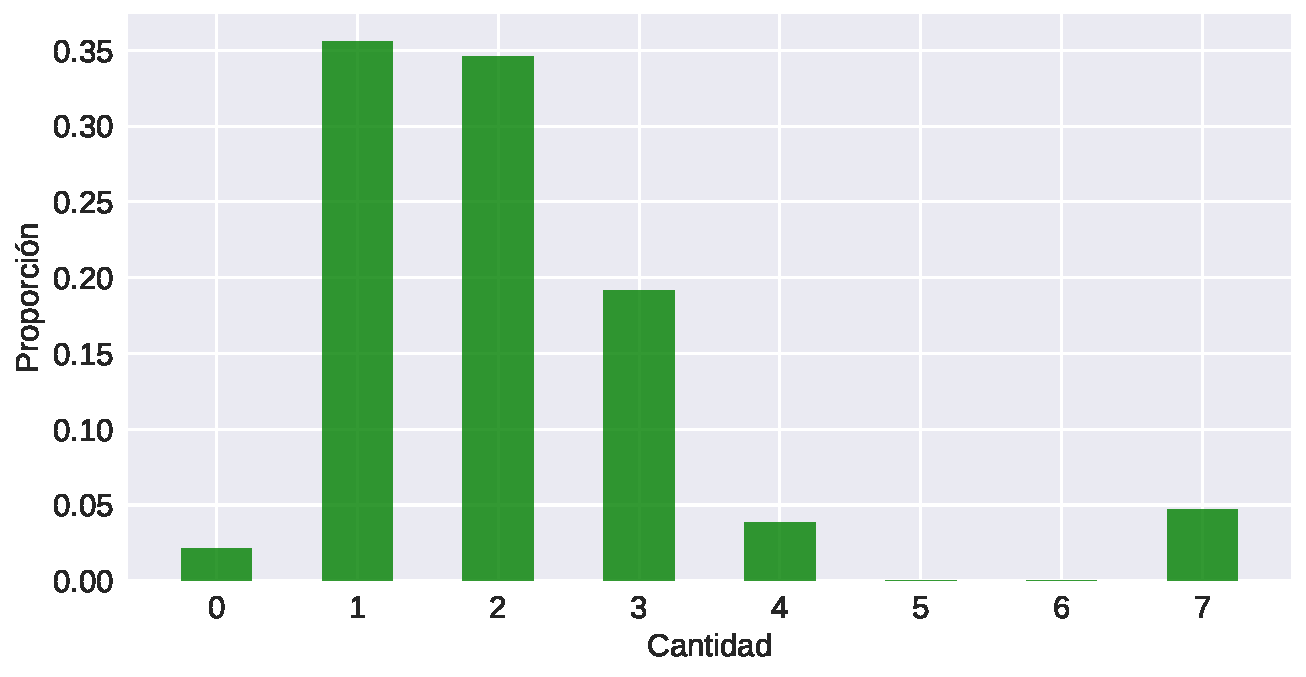
\includegraphics[scale=0.6]{documents/latex/figures/3/varq/nulos_varq.pdf}
    \caption{Histograma de cantidad de variables nulas por fila del dataset VarQ Curado.}
    \label{fig:nulos_varq}
\end{figure}

% \subsection{Correlación entre las variables de VarQ Curado}

También queremos conocer qué tan correlacionadas se encuentras las variables. En la figura \ref{fig:varq_corrplot} vemos la correlación de Spearman que sirve para detectar relaciones monotónicas entre las variables, y así nos permite descartar variables muy similares que no aportan nueva información y ralentizan el entrenamiento del modelo. De esta forma encontramos que la variable SASA y SASA\_PERCENTAGE tienen una correlación de 0.98. Mantuvimos las dos variables dado que la relativa baja cantidad de variables de este dataset no nos fuerza a removerlas, y si bien la correlación es muy alta, no descartamos a priori poder extraer información util usando ambas.

\begin{figure}[H]
    \centering
    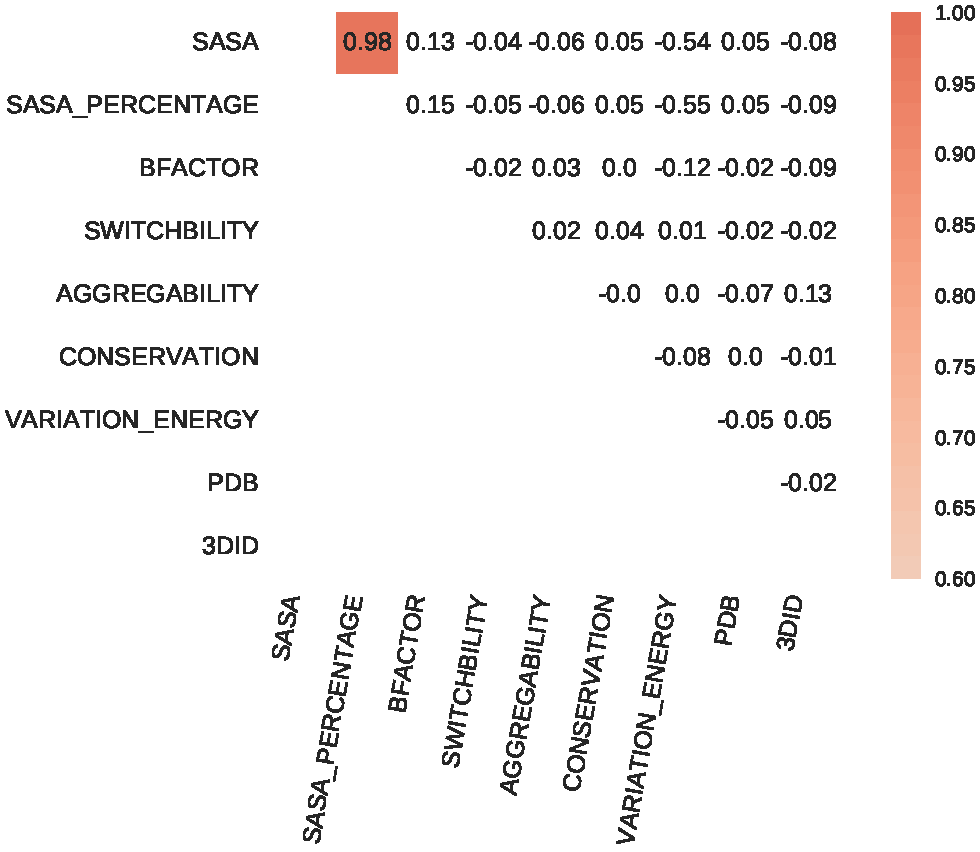
\includegraphics[scale=0.7]{documents/latex/figures/3/varq/varq_corrplot.pdf}
    \caption{Correlación de Spearman para las variables de VarQ Curado.}
    \label{fig:varq_corrplot}
\end{figure}

Finalmente en la tabla \ref{tab:descripcion_varq_cont} podemos ver distintas métricas sobre las variables continuas del dataset, como la media de los valores (mean), el desvío estándar (std), el valor máximo (max) y los cuartiles. 

En esta descripción sumamos el AUC univariado, es decir el área bajo la curva ROC tomando la variable ordenada como estimador de la respuesta.   

Un AUC cercano a 0.5 equivale a una variable de bajo poder predictivo, mientras que un AUC mayor a 0.5 corresponde a un predictor de la variable de respuesta (en este caso una variante patogénica), mientras que un AUC menor a 0.5 corresponde a un anti-predictor, es decir que invertir su respuesta equivale a un predictor de AUC mayor a 0.5. En la columna AUC de la tabla \ref{tab:descripcion_varq_cont} vemos que las variables SASA y SASA \% tienen un poder anti-predictivo relativamente alto (0.34 y 0.33 respectivamente), lo que indica que las variantes que tengan un valor elevado de estas variables tienden a ser benignas, mientras que la variación de energía tiene el mejor poder predictivo univariado entre todas las variables.

\begin{table}[H]
\centering
\begin{tabular}{|l|l|l|l|l|l|l|l|l|}
\hline
Variable & avg  & std   & min    & 25\%  & 50\%  & 75\%  & max & AUC\\ \hline
SASA    & 32.11 & 39.15 & 0.0    & 0.67  & 15.21 & 52.15 & 246.41 & 0.34 \\ \hline
SASA\%  & 0.15  & 0.18  & 0.0    & 0.0   & 0.07  & 0.27  & 0.75 & 0.33  \\ \hline
BFACTOR & 56.45 & 71.76 & 0.0    & 19.77 & 37.34 & 61.14 & 755.61 & 0.46 \\ \hline
SWITCH  & 0.38  & 0.89  & 0.0    & 0.0   & 0.01  & 0.28  & 8.72 &  0.50  \\ \hline
AGG     & 5.02  & 17.61 & 0.0    & 0.0   & 0.0   & 0.16  & 100.0 &  0.51\\ \hline
CONS    & 0.33  & 0.19  & 0.13   & 0.25  & 0.3   & 0.37  & 4.77 & 0.43\\ \hline
ENE     & 2.91  & 4.84  & -12.64 & 0.26  & 1.51  & 3.89 & 57.21 & 0.68\\ \hline 
\end{tabular}
\caption{Descripción de variables continuas del dataset \textit{VarQ Curado}.}
\label{tab:descripcion_varq_cont}
\end{table}

\begin{table}[H]
\centering
\begin{tabular}{|l|l|l|l|}
\hline
Variable & top  & freq. top & BACC \\ \hline
3DID & False & 0.8 & 0.51\\ \hline
PDB  & False  & 0.9 & 0.49\\ \hline
\end{tabular}
\caption{Descripción de variables categóricas del dataset \textit{VarQ Curado}.}
\label{tab:descripcion_varq_cat}
\end{table}

Para el caso de las variables categóricas (PDB y 3DID), analizamos el valor con la frecuencia más alta (top) y el valor de esta frecuencia. Para este tipo de variables quisimos también cuantificar su poder predictivo individual. 

% \newpage

Utilizar AUC en este caso no es posible dado que su cálculo sólo tiene sentido en variables continuas. Por lo tanto, decidimos calcular el \textit{Balanced Accuracy} (BACC) \cite{Brodersen2010} como medida de poder predictivo, considerando el valor de la variable como predictor de la variante.

El \textit{Balanced Accuracy} (BACC) es igual a:
\begin{equation*}
    \frac{1}{2} (\frac{VP}{P} + \frac{VN}{N})
\end{equation*}

Al igual que con el AUC, un valor mucho menor a 0.5 indica poder anti-predictivo, por lo que invertir la respuesta daría lugar a un buen predictor. En la tabla \ref{tab:descripcion_varq_cat} podemos ver que el BACC de las variables 3DID y PDB es de 0.51 y 0.49 respectivamente, lo que indica un bajo valor predictivo. 

% \newpage

\section{Modelo creado a partir del dataset VarQ Curado}

Una vez definido el dataset, podemos emplear técnicas de aprendizaje automático con el objetivo de generar un predictor de variantes patogénicas. Cabe destacar, que en este dataset VarQ Curado hay una sobrerrepresentación de variantes patogénicas, es decir, que presenta un desbalance (mayor número de variantes patogénicas que benignas) que invierte las propociones observadas en el dataset VarQ Completo. De todas formas generaremos un modelo para poder evaluar de forma preliminar la dificultad del problema. 

Para esto recurrimos a diferentes algoritmos de aprendizaje automático: Support Vector Classifier (SVC), Regresión Logística y Random Forest. La construcción del pipeline para cada uno de estos algoritmos constó de tres fases: 

\begin{itemize}
    \item \textbf{Creación del set de entrenamiento y de evaluación}: División (\textit{split}) estratificado (es decir, manteniendo las proporciones originales de la variable objetivoE) del dataset, 66\% para entrenamiento y 33\% para evaluación. 
    \item \textbf{Imputación de las variables}: Se reemplazaron los valores nulos de cada variable por su mediana en caso de las continuas y por el valor más frecuente en el caso de las variables categóricas.
    \item \textbf{Estandarización}: Para el caso de los algoritmos paramétricos (Regresión Logística y SVM) se aplicó una estandarización robusta a outliers. Esta estandarización consiste en restar la mediana del valor y escalar los datos de acuerdo a la distancia intercuartil, como se observa en la ecuación \ref{eq:robust_scaler}.
    
    \begin{equation}
        RobustScaling(x_i) = \frac{x_i - Q_2(\textbf{x})}{Q_3(\textbf{x}) - Q_1(\textbf{x})} 
        \label{eq:robust_scaler}
    \end{equation}
    
    donde $x_i$ corresponde al valor de la variable,  $Q_1$, $Q_2$ y $Q_3$ corresponde al primer, segundo y tercer cuartil de la variable $\textbf{x}$ respectivamente.
    
    
\end{itemize}

Luego del preprocesamiento, para cada uno de los algoritmos se realizó una búsqueda de hiperparámetros óptimos, a partir de estos datos, con la función \texttt{GridSearchCV} de la biblioteca \texttt{Scikit-learn} \cite{scikit-learn}. El objetivo de esta función es evaluar todas las combinaciones de hiperparámetros definidos en un diccionario y retornar el estimador que dio mejores resultados (de acuerdo a una métrica escogida, en este caso el área bajo la curva ROC). Esta métrica a su vez es evaluada a través de validación cruzada (\textit{3-fold Cross Validation}). En el apéndice se encuentran los diccionarios de hiperparámetros usados en cada uno de los modelos.

\section{Resultados}

Random Forest fue el mejor modelo con un AUC de 0.74. Los parámetros óptimos de este modelo fueron una profundidad de árbol de 7, 100 estimadores y una cantidad máxima de variables por árbol de 4. Denominaremos este modelo como Modelo VarQ Curado.

La Regresión Logística y SVC obtuvieron 0.71 y 0.70 de AUC respectivamente. Estos modelos se caracterizaron ademas por tener una tendencia a clasificar a las variantes como patogénicas, lo que se puede observar en su alto recall y menor precisión con respecto a Random Forest. En particular, SVC clasificó a todas las variantes del dataset de evaluación como patogénicas. También el tiempo de entrenamiento fue mucho mayor que el del resto de los algoritmos. En la tabla \ref{tab:metricsmodel} presentamos la Precisión y el Recall (con respecto a las variantes patogénicas) y el tiempo de entrenamiento del modelo y de predicción de todas las variantes del dataset de evaluación.

\begin{table}[H]
\centering
\begin{tabular}{|l|l|l|l|l|l|l|}
\hline
Modelo & Precisión & Recall & AUC & F1-score & $t_{fit}$ & $t_{pred}$ \\ \hline
SVC    & 0.72 & \textbf{1.00} & 0.70 & 0.84 & 2 m 39 s & 0.77s \\ \hline
LR     & 0.75 & 0.94 & 0.71 & 0.84 & \textbf{1.17 s} & \textbf{0.01 s} \\ \hline
RF     & \textbf{0.77} & 0.93 & \textbf{0.74} & 0.84 & 9.82 s & 0.11 s \\ \hline
\end{tabular}
\caption{Comparación de métricas de modelos usando el dataset VarQ Curado. Las variables $t_{fit}$ y $t_{pred}$ corresponden al tiempo de entrenamiento y de predicción de todas las variantes.}
\label{tab:metricsmodel}
\end{table}

La tabla \ref{tab:metrics_varq} muestra algunas métricas de interés obtenidas del modelo Random Forest para entender mejor los resultados del modelo basados en el predictor generado.

\begin{table}[H]
\centering
\begin{tabular}{|l|l|l|l|}
\hline
              & Precisión & Recall & F1-score \\ \hline
Benignas      & 0.57      & 0.26   & 0.36     \\ \hline
Patogénicas   & 0.77      & 0.93   & 0.84     \\ \hline
Promedio      & 0.71      & 0.74   & 0.71     \\ \hline
\end{tabular}
\caption{Reporte de métricas del modelo Random Forest usando el dataset VarQ Curado.}
\label{tab:metrics_varq}
\end{table}

La precisión del modelo indica un número marcadamente bajo (0.57) en la clase benigna, lo que significa que casi una de cada dos variantes detectadas como benignas es en efecto patogénica. El Recall con respecto a las variantes benignas es de 0.26, es decir que el modelo sólo reconoce alrededor de un cuarto de las variantes benignas como tales. Por lo tanto podemos afirmar que este modelo tiene una tendencia a clasificar las variantes como patogénicas, generando una gran cantidad de falsos positivos (o Error de tipo I). Es importante remarcar que estas métricas están generadas a partir de una función de decisión o \textit{threshold} fijado por la versión del algoritmo usado (en el caso de la biblioteca \texttt{scikit-learn}, este \textit{threshold} está ubicado en 0.5 de la probabilidad asignada).  La curva ROC, o \textit{Receiver Operating Characteristic} y su AUC asociada, nos permite independizarnos de un \textit{threshold} fijo para evaluar las características del predictor (figura \ref{fig:auc_varq}).

En la figura \ref{fig:importance_varq} podemos observar la importancia de los features reportado por el algoritmo Random Forest, que ubica en primer lugar con una gran diferencia a la variable que hace referencia a la Variación de Energía (ENE), seguido por el BFACTOR y el porcentaje de SASA (SASA \%). Este dato concuerda parcialmente con sus valores de AUC univariado (tabla \ref{tab:descripcion_varq_cont}). Si bien ENE y SASA \% poseen un valor relativamente alto de poder de clasificación univariada, no sucedía lo mismo con BFACTOR. En el modelo multivariado esta situación se invierte, con BFACTOR en el segundo lugar de importancia.

\newpage

\begin{figure}[H]
\centering
\begin{subfigure}{0.7\textwidth}
    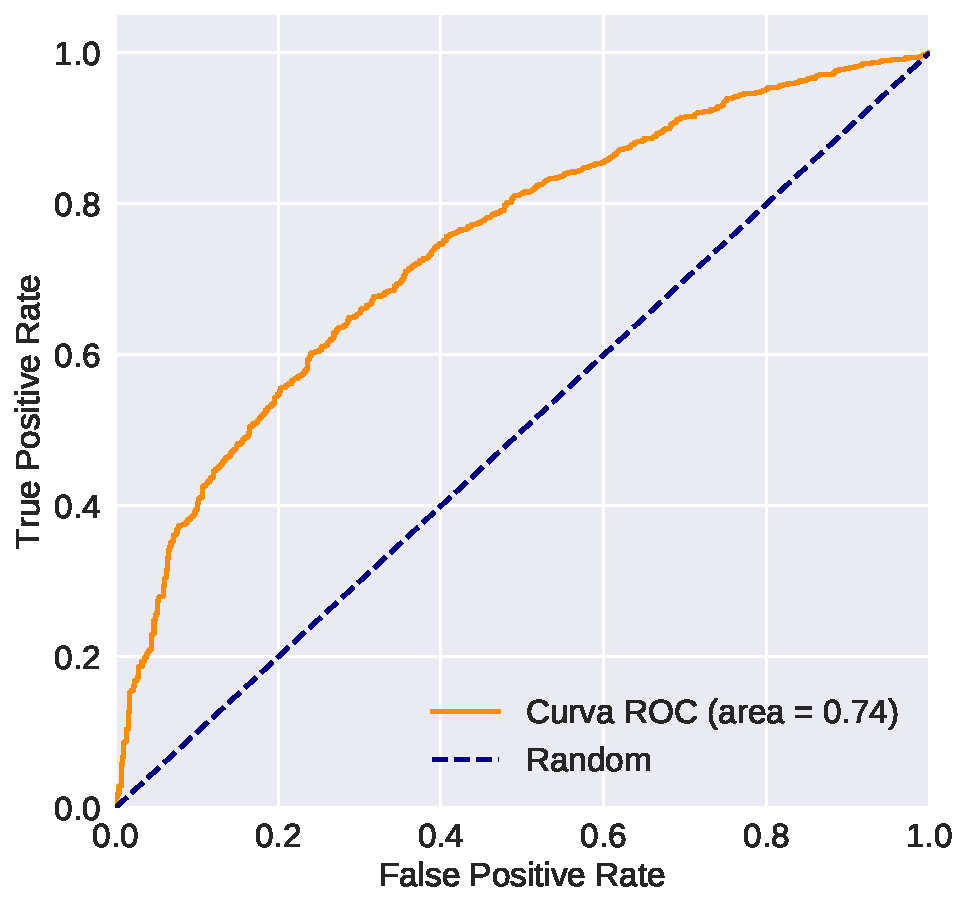
\includegraphics[width=\textwidth]{documents/latex/figures/3/varq/auc_varq.pdf}
    \caption{Curva ROC del modelo. La línea punteada corresponde a la curva ROC de un estimador aleatorio, o \textit{Random}, cuyo AUC es igual a 0.5.}
    \label{fig:auc_varq}
\end{subfigure}
\begin{subfigure}{0.7\textwidth}
    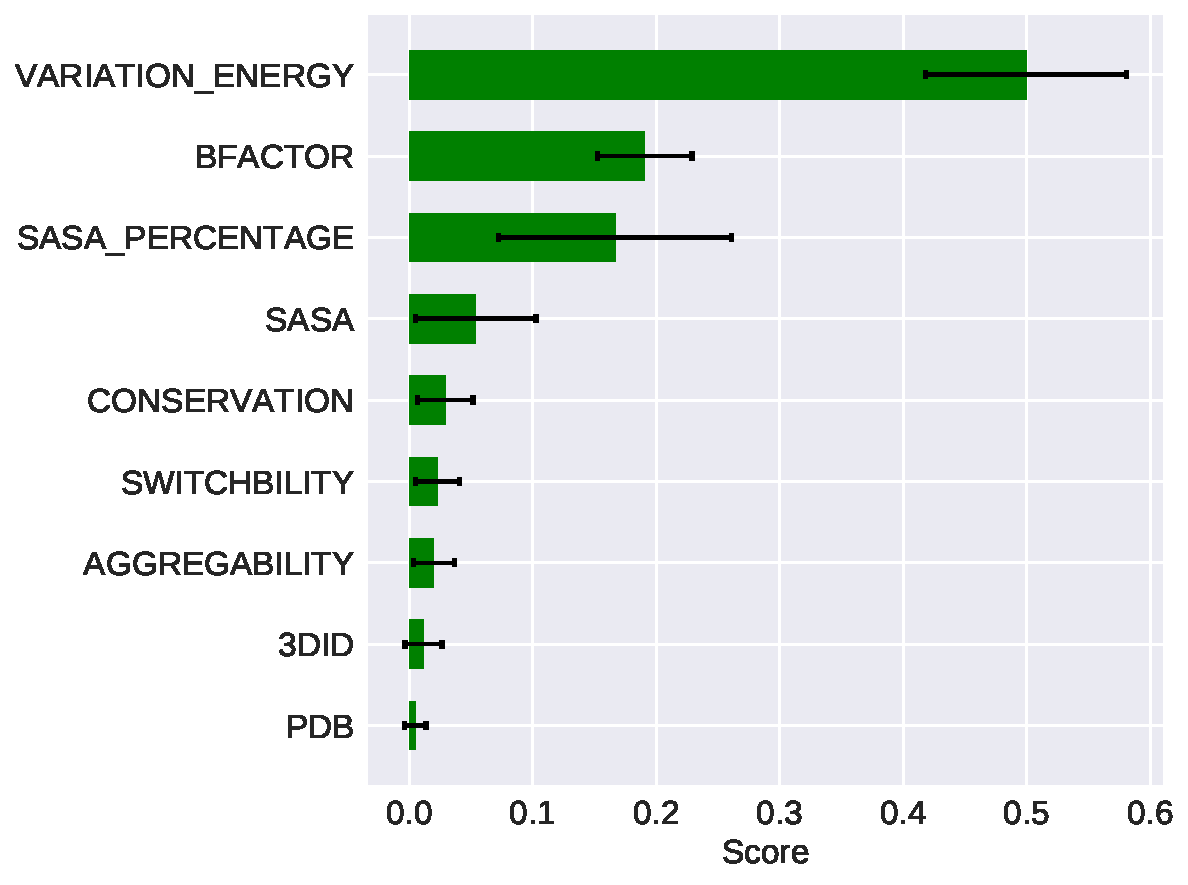
\includegraphics[width=\textwidth]{documents/latex/figures/3/varq/importances_varq.pdf}
    \caption{Los atributos del dataset VarQ Curado en orden de importancia. La barra de error corresponde al desvío estándar del \textit{Feature Importance} de cada uno de los árboles del modelo.}
    \label{fig:importance_varq}
\end{subfigure}

\caption{Curva AUC y atributos más importantes del Modelo VarQ Curado.}

\end{figure}

\chapter{Modelo usando propiedades físico-químicas de la proteína}
\label{ch:desarrollo_fisico_quimico}
% \section{Modelo usando propiedades físico-químicas de la proteína}

En esta sección generamos un nuevo dataset buscando fuentes complementarias de información de carácter físico-químico de las proteínas. Estas variables provienen de dos fuentes principales:

\begin{itemize}
    \item El módulo ProtParam proveniente de la biblioteca Biopython \cite{Chapman:2000:BPT:360262.360268}
    \item La base de datos SNVBox del laboratorio Karchin \cite{Wong2011}
\end{itemize}

Para el análisis de estas variables usamos únicamente la tabla Humsavar. La tabla Humsavar (versión 2017\_12) \cite{humsavar} está compuesta originalmente por 75,769 variantes (o ``mutantes'') de las cuales 39,653 son benignas (52\%), 28,855 (38\%) están asociadas a enfermedades y 7,261 (10\%) no están clasificadas. Las variantes no clasificadas fueron descartadas. Esta tabla tiene un tamaño de casi 10 veces la cantidad de variantes del dataset VarQ Curado, de aproximadamente 7400 variantes.

\section{Extracción de variables usando Biopython}

La primera fuente que utilizamos, por su relativa practicidad de uso en la extracción de un conjunto de variables físico-químicas de la proteína, fue el módulo ProtParam de la biblioteca Biopython. Esta biblioteca es un set de herramientas escritas en Python, desarrollada por un equipo internacional de desarrolladores para el área de la bioinformática, y posee una licencia de uso libre (Licencia Biopython \cite{biopython-license}).
El nombre ProtParam proviene de \textit{Protein Parameters} (parámetros de la proteína) y está basado en la herramienta homónima del server proteómico Expasy \cite{expasy}. Para poder acceder a los parámetros calculados el módulo requiere el \textit{accession number} de la proteína (identificador único) o una subsecuencia de la misma. Las variables obtenidas son las siguientes:

\begin{itemize}
    \item Punto isoeléctrico teórico (ISO\_POINT): pH en el que la proteína (o subsecuencia) tiene carga nula. 
    \item Aromaticidad (AROM): La frecuencia relativa de la subsecuencia Phe+Trp+Tyr (Fenilalanina, Triptófano y Tirosina). 
    \item Índice de inestabilidad (INST): Testea la estabilidad de la subsecuencia. Cualquier valor superior a 40 indica inestabilidad, es decir una corta semivida. 
    \item Flexibilidad (FLEX): Método de Flexibilidad implementado por Vihinen et Al \cite{vihinen1994}.  
    \item Promedio de hidrofobicidad (GRAVY): La suma de valores de hidrofobicidad de cada uno de los aminoácidos que componen la subsecuencia de la proteína.
\end{itemize}

% \newpage

Para poder utilizar el módulo ProtParam recurrimos a Uniprot \cite{uniprot} con el fin de conseguir el proteoma humano en formato FASTA \cite{FASTA}. El formato FASTA fue desarrollado por David Lipman y William Pearson en 1985, y originalmente fue incluido en un programa del mismo nombre utilizado para el alineamiento múltiple de secuencias. Un archivo FASTA puede incluir diferentes secuencias, no necesariamente de aminoácidos, y cada una de estas secuencias posee una línea de descripción al comienzo que empieza con el símbolo $>$. Por ejemplo, así se ve la secuencia de la Ovoalbúmina, una proteína de la especie Gallus gallus (gallina), o en otras palabras, la principal proteína que encontramos en la clara de sus huevos (ver figura \ref{code:fasta_code})

\begin{figure}[H]
% \centering
    \begin{verbatim}
    	>P01013 GENE X PROTEIN (OVALBUMIN-RELATED)
    	QIKDLLVSSSTDLDTTLVLVNAIYFKGMWKTAFNAEDTREMPFHVTKQESKPVQMMCMNNSFNVATLPAE
    	KMKILELPFASGDLSMLVLLPDEVSDLERIEKTINFEKLTEWTNPNTMEKRRVKVYLPQMKIEEKYNLTS
    	VLMALGMTDLFIPSANLTGISSAESLKISQAVHGAFMELSEDGIEMAGSTGVIEDIKHSPESEQFRADHP
    	FLFLIKHNPTNTIVYFGRYWSP
    \end{verbatim}
% \includegraphics{}
\caption{Ejemplo de código Fasta. Este código representa la proteína albúmina, donde cada letra representa un aminoácido, por ejemplo, las primeras 5 letras representan Q (glutamina), I (isoleucina), K (lisina), D (ácido aspártico) y L (leucina).}
\label{code:fasta_code}

\end{figure}
% \pagebreak

A partir del proteoma obtenido se extrajeron las secuencias correspondientes a las proteínas del dataset Humsavar, y para cada una de ellas se tomó una subsecuencia de la misma de 7 aminoácidos de largo, alrededor de la posición donde se produjo la variante (ver figura \ref{fig:sequence_window}). Tomamos este largo en particular de acuerdo a su capacidad para reconocer estruturas hidrofílicas de acuerdo al trabajo de Gasteiger et al. \cite{Gasteiger2005}, aunque dejamos para trabajos futuros la exploración de otros largos de subsecuencia. 

En caso de que la variante se haya producido en los primeros o los últimos lugares, se toman aminoácidos a derecha o a izquierda según corresponda para completar el largo de la ventana.

% \begin{figure}
% \begin{textopo}
%   \labelstyle{hl}{diamond}{Black}{Blue}{White}{}
%   \sequence{PQALPSV[LQIAMAFGLAIGTLVQALG]HV%
%   SGAH[([NNE,30]hl[box[Black,Blue]:Half loop[White]]=INPAVTVACL)]VGCHVSFLR}
%   \Nterm{extra} \hideNterm \hideCterm \hidelegend \labelTM{1}{II}
%   \labeloutside[right]{extra}
% \end{textopo}
% \caption{A `half loop' example}\label{fighalf}
% \end{figure}

\begin{figure}[H]
    \centering
    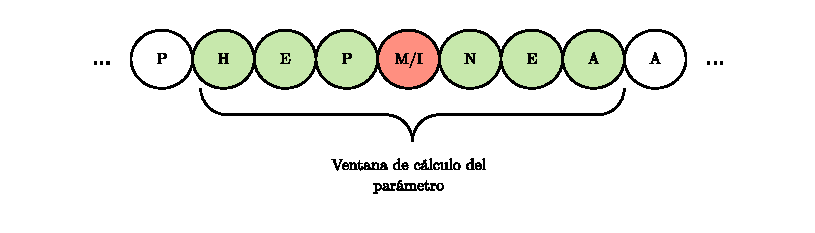
\includegraphics[width=\textwidth]{documents/latex/figures/3/structural/protparam.pdf}
    \caption{Secuencia de aminoácidos de la proteína Arilacetamida deacetilasa (Q5VUY0). La ventana de la subsecuencia está marcada en verde, y la posición rojo es la mutación estudiada. En este caso la metionina (M) en la posición 307 fue reemplazada por una isoleucina (I).}
    \label{fig:sequence_window}
\end{figure}

A partir de los parámetros calculados en ProtParam, buscamos capturar la magnitud del cambio debido a la variante. Estos cambios pueden ser responsables de un efecto patogénico. Por ejemplo, si la región afectada por la variante pasa a ser hidrofílica en vez de hidrofóbica esta será más propensa a efectos adversos \cite{doi:10.1093/bioinformatics/btt308}.

% \newpage

En este sentido, generamos dos variables que buscan reflejar la diferencia generada por la variante. Las variables son las siguientes: 

\begin{itemize}
    \item Diferencia (DIFF) 
    $$|x - x_{var}|$$
    \item Cociente de logaritmos (LOG\_RATIO)
    $$\frac{\log{(x + 1)}}{\log{(x_{var} + 1)}}$$  
\end{itemize}

donde $x$ representa al parámetro original y $x_{var}$ es igual al parámetro de la variante.

\section{Extracción de variables usando SNVBox}

Además de la información obtenida vía ProtParam, recurrimos a una base de datos llamada SNVBox. Esta base de datos fue elaborada y es actualmente mantenida por el Karchin Lab de la Universidad Johns Hopkins. Se encuentra en su versión 3.0 y sigue actuallmente en desarrollo. SNVBox posee alrededor de 90 variables consideradas relevantes para detectar el impacto biológico de un SNV (\textit{Single Nucleotide Variant}). Si bien existen distintos criterios para definir un SNV y su diferencia de un SNP (basados en la frecuencia del alelo menos común o MAF por sus siglas en inglés), en este trabajo los usaremos de forma indistinta. SNVBox posee datos físico-químicos de la proteína, a nivel de aminoácido y también a nivel de los sitios de la proteína donde se encuentra la variante. Otra característica destacable de esta fuente es que posee dichas variables para todos los codones del exoma humano. En el apéndice (ver sección \ref{snvbox_list}) se encuentra el listado de variables extraídas con su descripción.

\section{Generación del dataset Físico-Químico}

Luego del proceso del extracción de variables de Biopython y SNVBox, generamos un nuevo dataset cruzando sus atributos con las variantes registradas en Humsavar. En el caso de los atributos relativos a los aminoácidos, pudimos cruzarlos usando la columna del dataset referente al identificador de la proteína, la posición de la variante, y el par de aminoácidos que se intercambiaron. Una vez agregadas todas las variantes a la tabla Humsavar, removimos todas aquellas variantes sin clasificación (etiqueta \textit{Unclassified}). El dataset resultante (denominado dataset Físico-Químico) está compuesto por 68,508 observaciones y 50 variables, incluyendo la variable de respuesta (o tipo), de las cuales 39,653 son benignas (58\%), y 28,855 (42\%) variantes están asociadas a alguna enfermedad. 

% Este dataset estará puesto a disposición para su libre uso. 

\section{Descripción estadística del dataset Físico-Químico}

Luego de la creación del dataset realizamos una exploración estadística del mismo, tal como hicimos en el dataset VarQ Curado. Calculamos la media (\textit{mean}), el desvío estándar (\textit{std}), el mínimo, el máximo y los cuartiles (25\%, 50\%, y 75\%). En la tabla \ref{tab:protparam_vars} podemos ver que la variable GRAVY\_LOG\_RATIO se encuentra en una escala muy distinta a la de las demás variables, por lo que en algunos algoritmos es necesario escalar las variables (por ejemplo en la regresión logística). En el caso de la variable INST\_LOG\_RATIO si bien la media y la mediana son muy parecidas los valores mínimos y máximos estan muy alejados de la distancia intercuartil (tercer cuartil menos el primero), por lo que podemos afirmar que son valores atípicos o \textit{outliers}.

También calculamos el AUC univariado para cada una de las variables continuas del dataset. Con respecto al AUC univariado en las variables de Protparam (ver tabla \ref{tab:protparam_vars}), notamos que la versión DIFF de los parámetros es mejor (anti) predictor que sus versiones LOG\_RATIO en todos los casos.


\begin{table}[H]
\centering
\begin{tabular}{|l|l|l|l|l|l|l|l|l|}
\hline
Variable & mean & std & min & 25\% & 50\%  & 75\% & max & AUC \\ \hline
AROM\_DIFF  & 0.02  & 0.02  & 0.00 & 0.00 & 0.00  & 0.01 & 0.22  & 0.59 \\ \hline
AROM\_LOG\_RATIO & 1.97 & 0.33 & 1.00 & 1.94 & 1.94  & 1.94 & 3.66  & 0.53 \\ \hline
ISO\_POINT\_DIFF & 0.69  & 0.98 & 0.00  & 0.00 & 0.17  & 1.22 & 6.30  & 0.56 \\ \hline
ISO\_POINT\_LOG\_RATIO & 2.00 & 0.08 & 1.69 & 1.99 & 2.00  & 2.01 & 2.45  & 0.51 \\ \hline
GRAVY\_DIFF & 0.23 & 0.17 & 0.00 & 0.09 & 0.20  & 0.33 & 1.67  & 0.55 \\ \hline
GRAVY\_LOG\_RATIO & 2x10$^{12}$ & 1.2x$10^{14}$ & -3.3x10$^{15}$ & 1.43 & 1.94 & 2.43 & 9.6x10$^{15}$ & 0.48 \\\hline
INST\_DIFF & 14.02 & 13.27 & 0.00 & 4.20 & 10.09 & 20.10 & 139.00 & 0.49 \\ \hline
INST\_LOG\_RATIO & 2.06 & 2.27 & -84.77 & 1.96 & 2.01  & 2.09 & 453 & 0.48 \\ \hline
FLEX\_DIFF & 0.01 & 0.01 & 0.00 & 0.00 & 0.01  & 0.01  & 0.05 & 0.54 \\ \hline
FLEX\_LOG\_RATIO & 2.00 & 0.01 & 1.97 & 1.99 & 2.00  & 2.01  & 2.03 & 0.47 \\ \hline
\end{tabular}
\caption{Variables extraídas de Protparam correspondientes al Dataset Físico-Químico.}
\label{tab:protparam_vars}
\end{table}

% \newpage

Con respecto al AUC univariado de las variables extraídas de SNVBox, notamos que las mejores variables en este respecto son las aportadas por algunas de las matrices de sustitución (EX, PAM250 y BLOSUM). En este caso son buenos anti-predictores, lo que indica que un valor bajo en esta matriz aporta una mayor probabilidad de ser patogénica (ver tabla \ref{tab:snvbox_amino}). El mejor predictor en este set de variables es el valor en la matriz de distancias GRANTHAM.  

% \newpage

% \subsection{Variables extraídas de SNVBox relativas a sustitución de aminoácidos}

\begin{table}[H]
\centering
\begin{tabular}{|l|l|l|l|l|l|l|l|l|}
\hline
Variable & mean   & std    & min    & 25\%  & 50\%   & 75\% & max & AUC    \\ \hline
CHARGE            & 0.00  & 0.71   & -2.00  & 0.00  & 0.00   & 0.00 & 2.00 & 0.50   \\ \hline
VOLUME            & -0.16  & 1.70   & -5.59  & -1.40 & -0.16  & 0.96 & 5.59 & 0.48   \\ \hline
HYDROPHOBICITY    & -0.63  & 6.81   & -15.70 & -3.10 & -0.40  & 1.90 & 15.70 & 0.52  \\ \hline
GRANTHAM          & 79.96  & 48.06  & 5.00   & 43.00 & 74.00  & 102.00 & 215.00 &  \textbf{0.63} \\ \hline
POLARITY          & -0.25  & 2.72   & -8.10  & -2.20 & -0.10  & 1.10   & 8.10 & 0.52   \\ \hline
EX                & 28.99  & 10.95  & -1.00  & 21.00 & 29.00  & 35.00  & 61.00 & \textbf{0.35}  \\ \hline
PAM250            & 0.16   & 1.68   & -5.40  & -1.00 & 0.20   & 1.40   & 5.30 & \textbf{0.36}   \\ \hline
BLOSUM            & -0.58  & 1.65   & -4.00  & -2.00 & -1.00  & 1.00   & 3.00 & \textbf{0.35}   \\ \hline
JM                & 0.80   & 1.24   & -1.73  & -0.50 & 1.05   & 1.66   & 3.22 & 0.40   \\ \hline
VB                & 19.78  & 14.64  & 0.00   & 8.00  & 17.00  & 29.00  & 55.00 & 0.42  \\ \hline
TRANSITION        & 0.00   & 0.00   & 0.00   & 0.00  & 0.00   & 0.00   & 0.01 & 0.47   \\ \hline
\end{tabular}
\caption{Variables extraídas de SNVBox relativas a sustitución de aminoácidos correspondientes al Dataset Físico-Químico.}
\label{tab:snvbox_amino}

\end{table}

Las variables continuas poseen una cobertura para el 100\% del dataset exceptuando algunas variables calculadas por ProtParam por alcanzar valores extremos (las cuatro variables LOG\_RATIO), en los que se decidió reemplazar por nulos. En la figura \ref{fig:proporcion_nulos_structural} presentamos la proporción de nulos en dichas variables.

Describimos 21 variables continuas de nuestro dataset. Las 29 variables restantes son extraídas de SNVBox relativas a proteínas y son todas categóricas de tipo \textit{Boolean} por lo que destacamos algunos datos de relevancia (ver sección 7.3 del apéndice para un listado completo). 

Todas estas variables tienen una cobertura para aproximadamente el 31.5\% de las variantes del dataset, y cada una de ellas poseen valor Falso para un porcentaje superior al 90\% de las variantes de la tabla, exceptuando las variables \textbf{TRANSMEM} (82\%), \textbf{REP} (87\%), \textbf{REGIONS} (70\%) y \textbf{PPI} (87\%). La descripción de estas variables se encuentra en el apéndice (ver sección \ref{snvbox_list}). 

\begin{figure}[H]
    \centering
    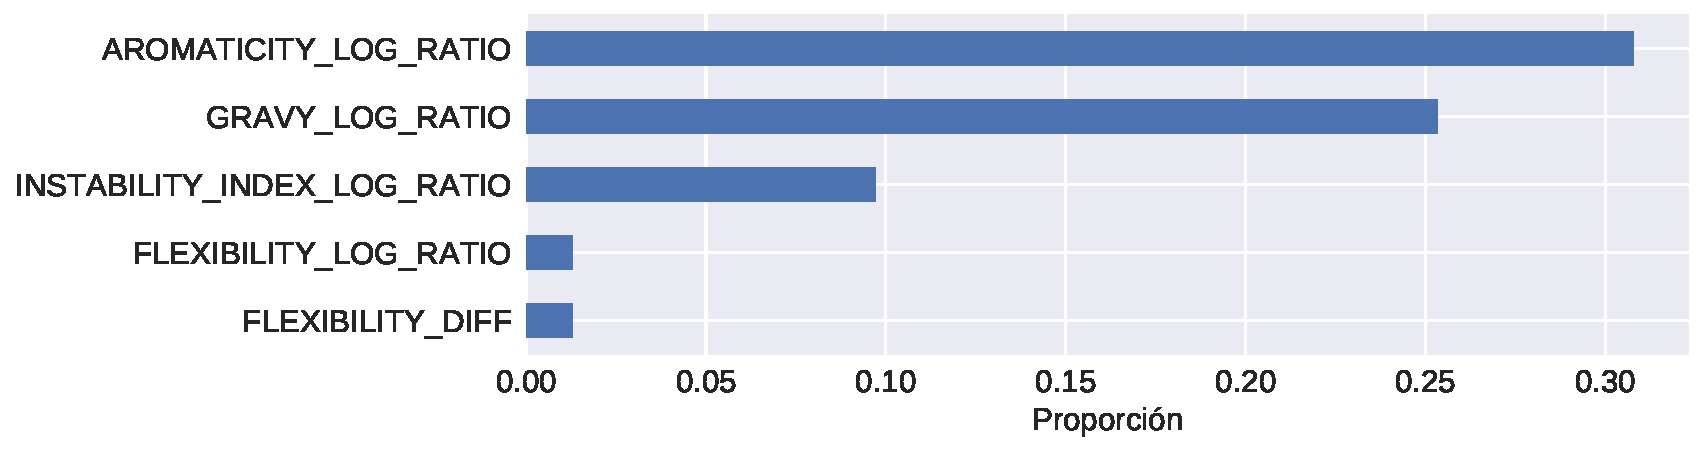
\includegraphics[scale=0.5]{documents/latex/figures/3/structural/proporcion_nulos_structural.pdf}
    \caption{Variables continuas con menor cobertura.}
    \label{fig:proporcion_nulos_structural}
\end{figure}

El \textit{Balanced Accuracy} de estas variables oscilan entre el 0.45 y 0.48, lo que connota un bajo poder predictivo univariado.
Por último, deseamos analizar la correlación entre las variables. Para esto usamos la correlación de Spearman dado que nos permite identificar correlaciones monotónicas. En la figura \ref{fig:corrplot_structural} podemos apreciar un cluster principal de variables altamente correlacionadas: Las matrices de sustitución (GRANTHAM, BLOSUM, JM, y EX).

% \newpage

\begin{figure}[H]
    \centering
    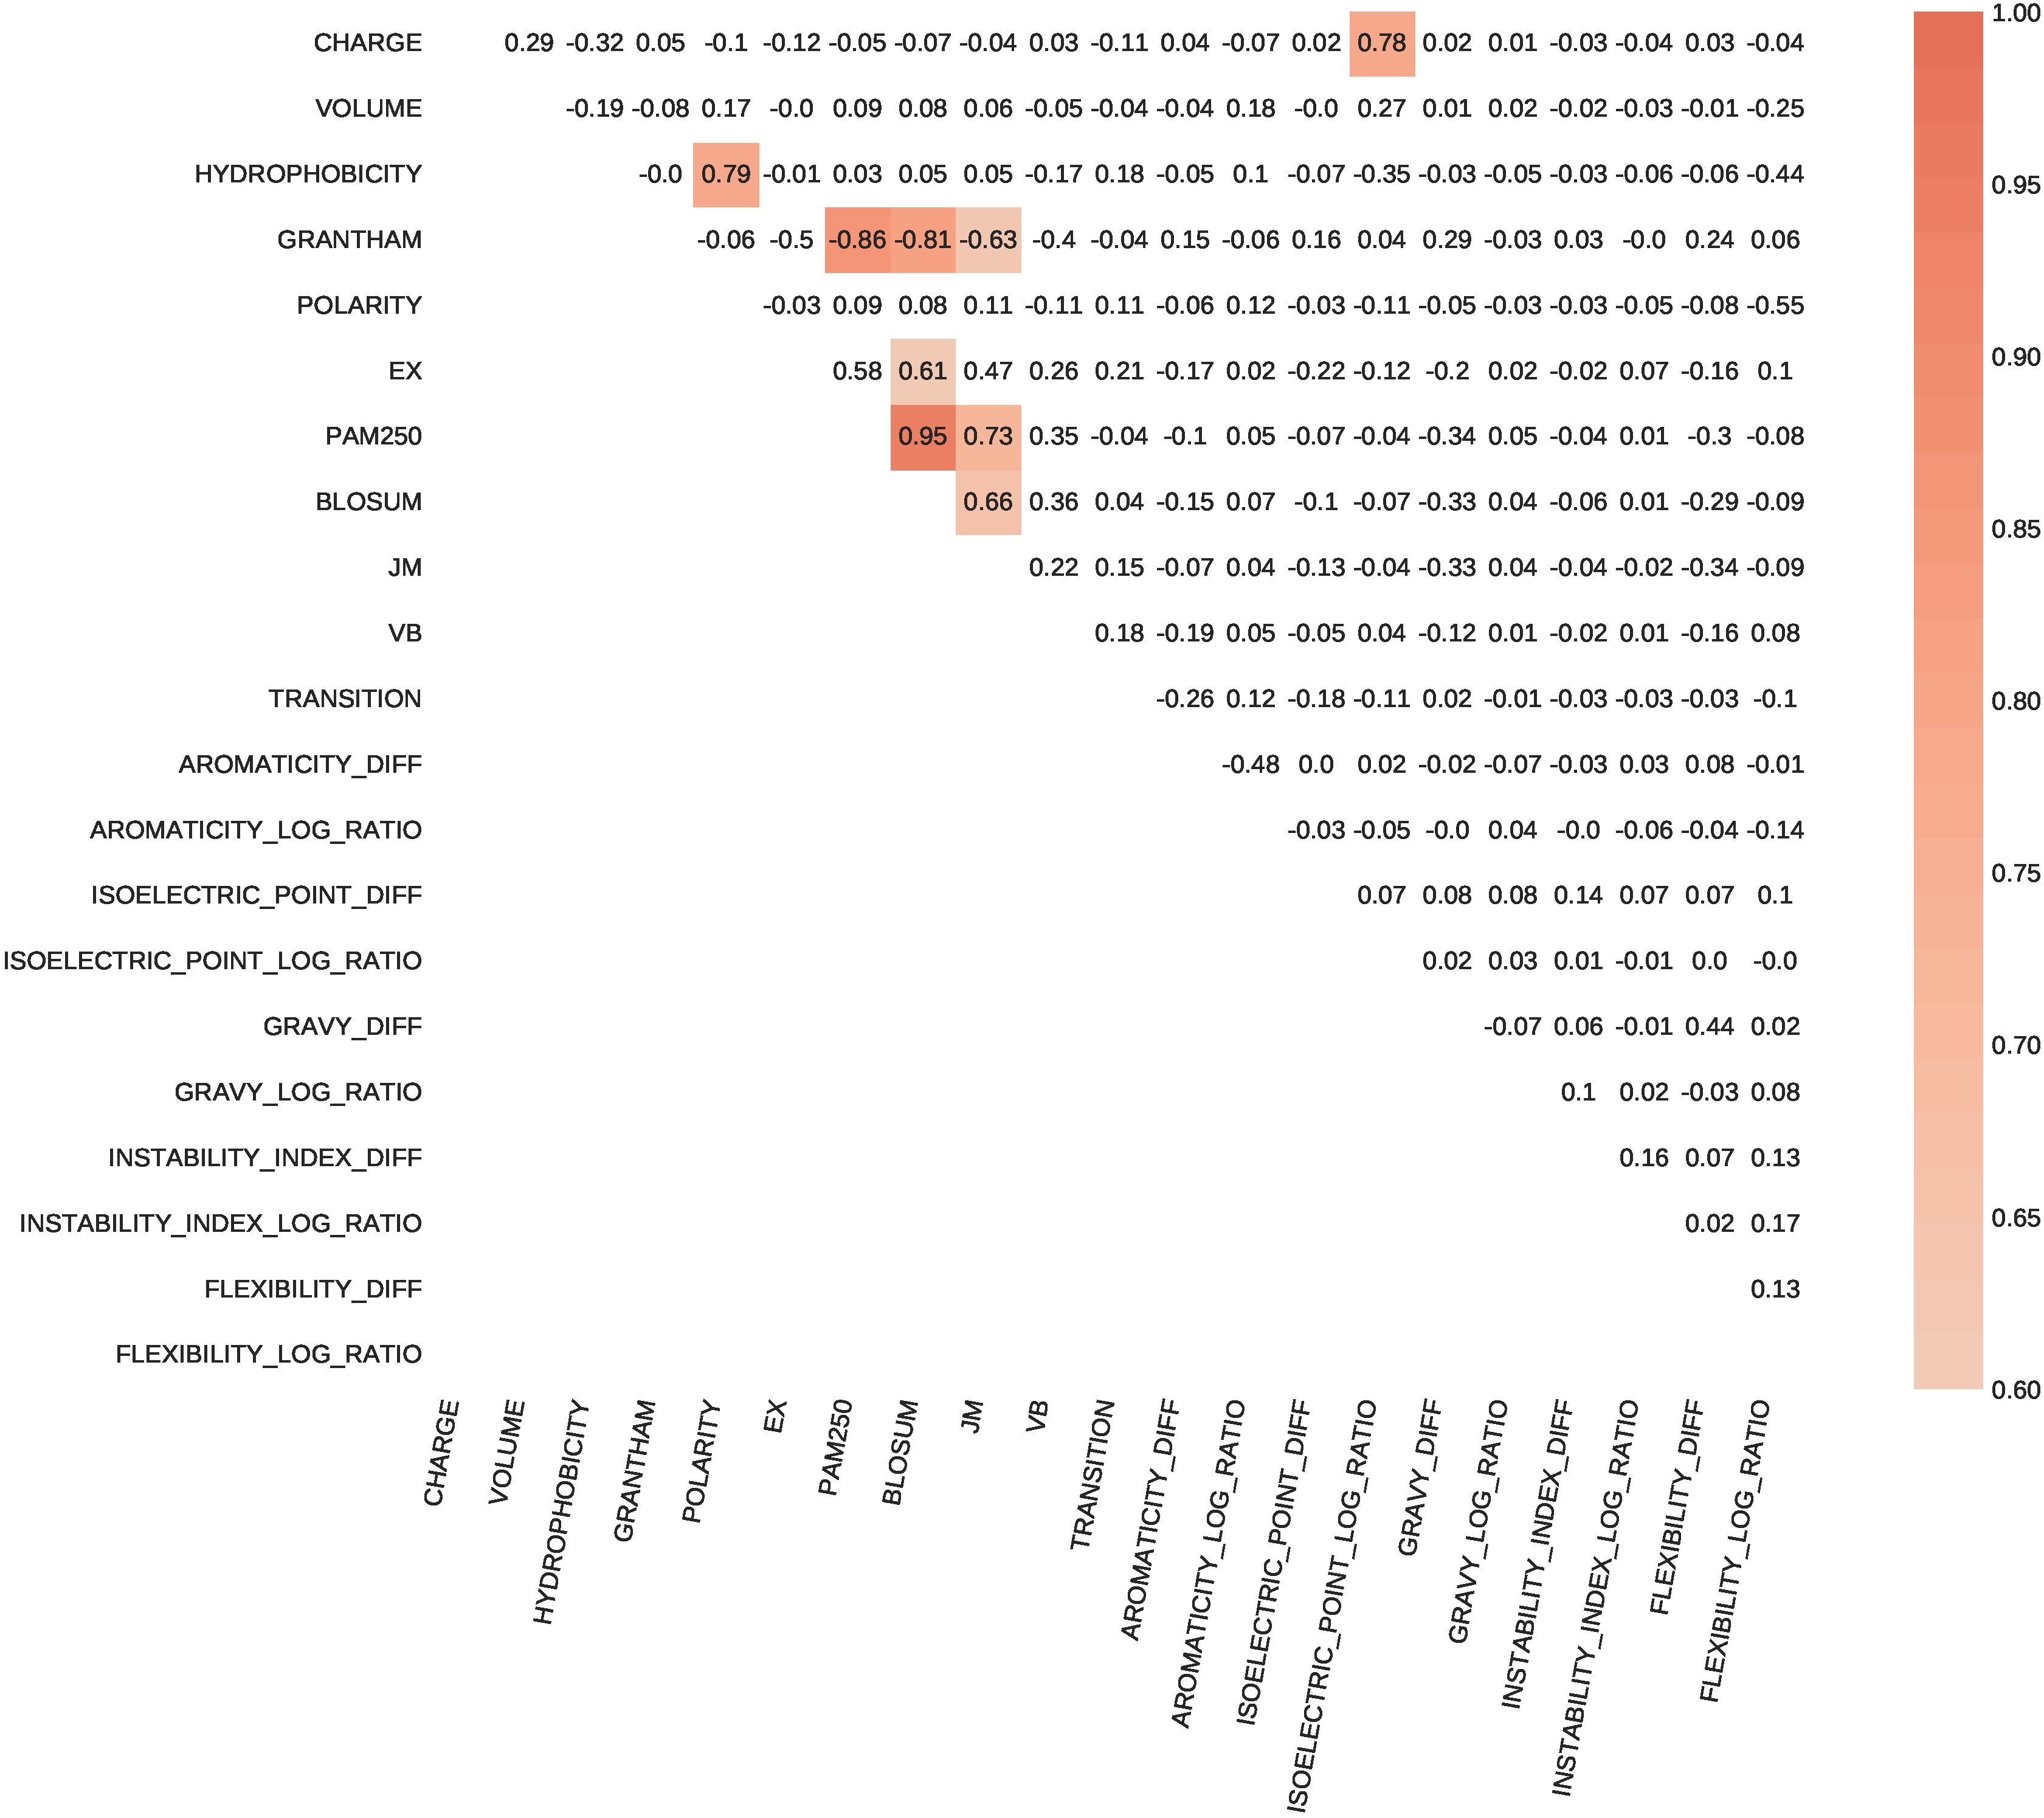
\includegraphics[scale=0.242]{documents/latex/figures/3/structural/structural_corr.pdf}
    \caption{Correlación de Spearman para las variables continuas del dataset Físico-Químico.}
    \label{fig:corrplot_structural}
\end{figure}



% \newpage
% \subsection{Correlación entre las variables}


Por otro lado, encontramos a las variables POLARITY e HYDROPHOBICITY correlacionadas entre sí (0.79), como también a las variables CHARGE e ISOELECTRIC\_POINT\_LOG\_RATIO (0.78). Para este análisis decidimos excluir a las variables categóricas por tratarse de variables de tipo binarias con baja cobertura, aunque de todas formas también fueron incluidas al modelo.  


% \subsection{Análisis de reducción de dimensionalidad}

% Una de las formas que nos permite ver que tan bien las variables de este dataset están separando nuestros tipos de SNPs, es usar reducción de dimensionalidad. El primer método que probamos fue el análisis de componentes principales (PCA), con el que generamos dos componentes, que son combinaciones lineales de nuestras variables iniciales de forma de maximizar la varianza, es decir el par de componentes que mejor explican la información completa.


% \newpage


\section{Generación del modelo}

Con este dataset generamos un modelo basado en un predictor Random Forest. 
Se eligió inicialmente este tipo de predictor por ser el que obtuvo los mejores resultados en el dataset VarQ Curado con respecto a otros predictores (SVMs y Regresión Logística). Otras de las ventajas que aporta este modelo es su facilidad para explicar la importancia de las variables y su relativa baja complejidad computacional, aunque es necesario tener cuidado al respecto con las correlaciones presentes entre las variables.

Para generar el modelo volvimos a construir un \textit{pipeline} muy similar al de la sección anterior, que consta de las siguientes etapas:

\begin{itemize}
 
\item \textbf{Imputación}: Las variables, cuyos valores eran nulos, se imputaron usando la mediana en el caso de las variables continuas, y con el valor más frecuente para las variables categóricas. 
\item \textbf{Escalado}: Las variables no fueron escaladas al no ser necesario en algoritmos de clasificacion basados en árboles de decisión, dado que se evalúan las variables de forma independiente. 
\item \textbf{Búsqueda de Hiperparámetros}: Para la búsqueda de hiperparámetros usamos \textit{Grid-Search} (búsqueda ``en cuadrícula''). El diccionario de hiperparámetros de cada uno de los algoritmos se encuentran en la sección 7.3 del apéndice.
\end{itemize}

Reutilizaremos este \textit{pipeline} en las próximas instancias en las que usemos algoritmos basados en árboles, al que denominaremos Pipeline Tree. 

\section{Resultados del modelo Físico-Químico}

Como puede observarse en la figura \ref{fig:auc_structural}, a partir de este modelo se obtuvo un AUC de 0.72. Este resultado es superior a los AUCs univariados del dataset (0.35, o 0.65 si consideramos su predicción inversa), cuyos mejores valores fueron aportados por las matrices de sustitución. A su vez este modelo es superado por el modelo VarQ Curado, lo que tiene sentido si consideramos que el poder de predicción de sus variables es superior a las de este  dataset, con 0.33 (o 0.67) en el caso de SASA y 0.68 en el caso de la variación de la energía (ENE).

El mejor modelo escogido durante la fase de entrenamiento posee profundidad de árbol (\texttt{max\_depth}) 7, 20\% de la cantidad de variables en cada corte (\texttt{max\_features}), y 100 árboles (\texttt{n\_estimators}). 

Las métricas observadas en la tabla \ref{structural_table} permiten dar cuenta de una precisión del 65\% con respecto a las observaciones patogénicas, es decir, el modelo está reportando un 35\% de variantes como patogénicas que no lo son (también conocido como error de tipo I), y un recall de 47\%, lo que indica que existe un 53\% de variantes patogénicas en nuestro dataset que no están siendo detectadas por nuestro modelo (error de tipo II). 

\begin{table}[H]
\centering
\begin{tabular}{|l|l|l|l|}
\hline
              & Precisión & Recall & F1-score \\ \hline
Benignas      & 0.68      & 0.81   & 0.74     \\ \hline
Patogénicas   & 0.65      & 0.47   & 0.54     \\ \hline
Promedio      & 0.66      & 0.67   & 0.66     \\ \hline
\end{tabular}
\caption{Métricas del modelo Random Forest aplicado al dataset Físico-Químico.}
\label{structural_table}
\end{table}

Si bien estos resultados son inferiores a los del modelo VarQ Curado, este modelo posee un Recall y Precisión de la clase benigna muy superior (0.81 vs. 0.26 y 0.68 vs 0.57 respectivamente), por lo que podemos afirmar que este modelo se encuentra más balanceado en la predicción de las clases, usando el \textit{threshold} proporcionado por \texttt{scikit-learn}.

\section{Importancia de los atributos}

El algoritmo Random Forest nos permite identificar los mejores atributos en cada uno de los árboles del clasificador. En este caso, los primeros cuatro atributos refieren a matrices de sustitución (ver figura \ref{fig:importances_structural}). La quinta variable en importancia pertenece a ProtParam (AROMATICITY\_DIFF). También en la figura \ref{fig:importances_structural}, se observan variables con un nivel de importancia muy similar, como es el caso de PAM250, EX, BLOSUM y GRANTHAM. Todas estas variables corresponden a matrices de sustitución. Esto último no es de extrañar ya que existe un alto nivel de correlación entre ellas (ver figura \ref{fig:corrplot_structural}). Como mencionamos en la sección 1.2.1 (Random Forest), el score de importancia de las variables es proporcional a la importancia máxima de todas las variables. En este caso, al haber una gran cantidad de variables correlacionadas entre sí, distribuimos el score entre ellas y perdemos la importancia que pueden estar aportando otras variables al modelo. 

Para solucionar este problema, acudimos a la herramienta \texttt{rfpimp} desarrollada por Terrence Parr et al. \cite{rfpimp}, que toma a su vez ideas del paper de Altmann et al. \cite{Altmann2010}. Esta herramienta permite agrupar variables y analizar su importancia realizando permutaciones aleatorias entre los ítems (SNPs), de forma de transformarlas en variables \textit{random}. Esta permutación genera una perdida de \textit{accuracy} en el modelo, que considera su nivel de importancia. El Accuracy se define como la cantidad de predicciones correctas dividido la cantidad de predicciones. Para generar clusters de variables observamos su nivel de correlación usando la correlación de Spearman, y agrupamos las variables que tenían una correlación mayor a 0.60. Eso nos dejo con tres clusters principales: Uno generado por HYDROPHOBICITY y POLARITY, otro por CHARGE y ISOELECTRIC\_POINT\_RATIO y por último otro generado por las matrices de sustitución (GRANTHAM, EX, PAM250, BLOSUM, JM y VB). 

Usando \texttt{rfpimp} (ver figura \ref{fig:importances_structural_cluster}) vemos más claramente como las matrices de sustitución toman un enorme rol en el desempeño del modelo, seguido por el par HYDROPHOBICITY y POLARITY. También aparecen nuevas variables en nivel de importancia, como DNA\_BIND y TRANSMEM (Sitio de unión de la proteína y región transmembrana respectivamente).


\newpage

\begin{figure}[H]
    \centering
    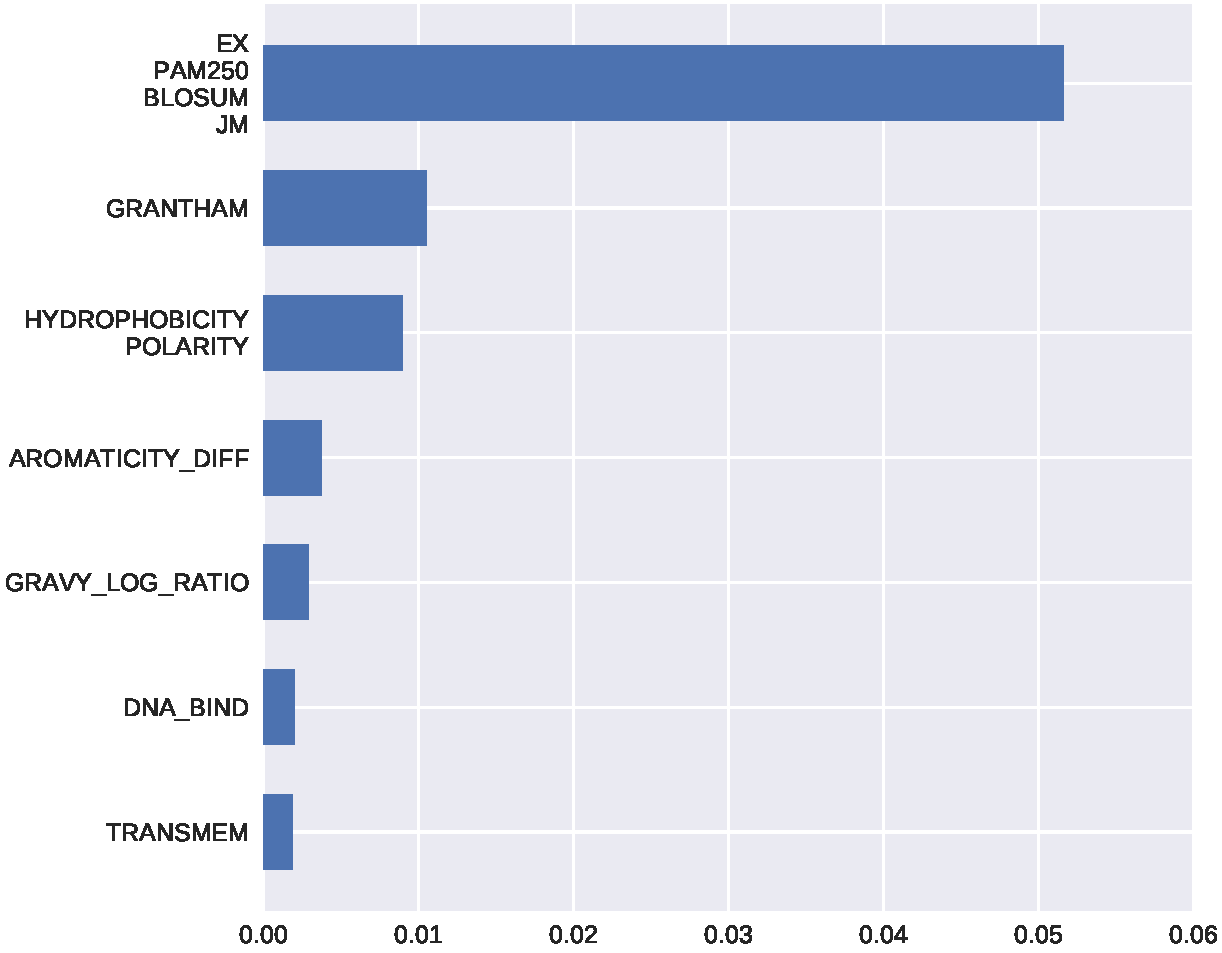
\includegraphics[scale=0.7]{documents/latex/figures/3/structural/structural_importance_cluster.pdf}
    \caption{Variación en el Accuracy al permutar clusters de variables altamente correlacionadas. Se agruparon variables con una correlación de Spearman superior a 0.60 y también se agruparon las matrices de sustitución EX, PAM250, BLOSUM, JM, GRANTHAM y VB.}
    \label{fig:importances_structural_cluster}
\end{figure}



\begin{figure}[H]
\centering
\begin{subfigure}[b]{0.7\textwidth}
    \centering
    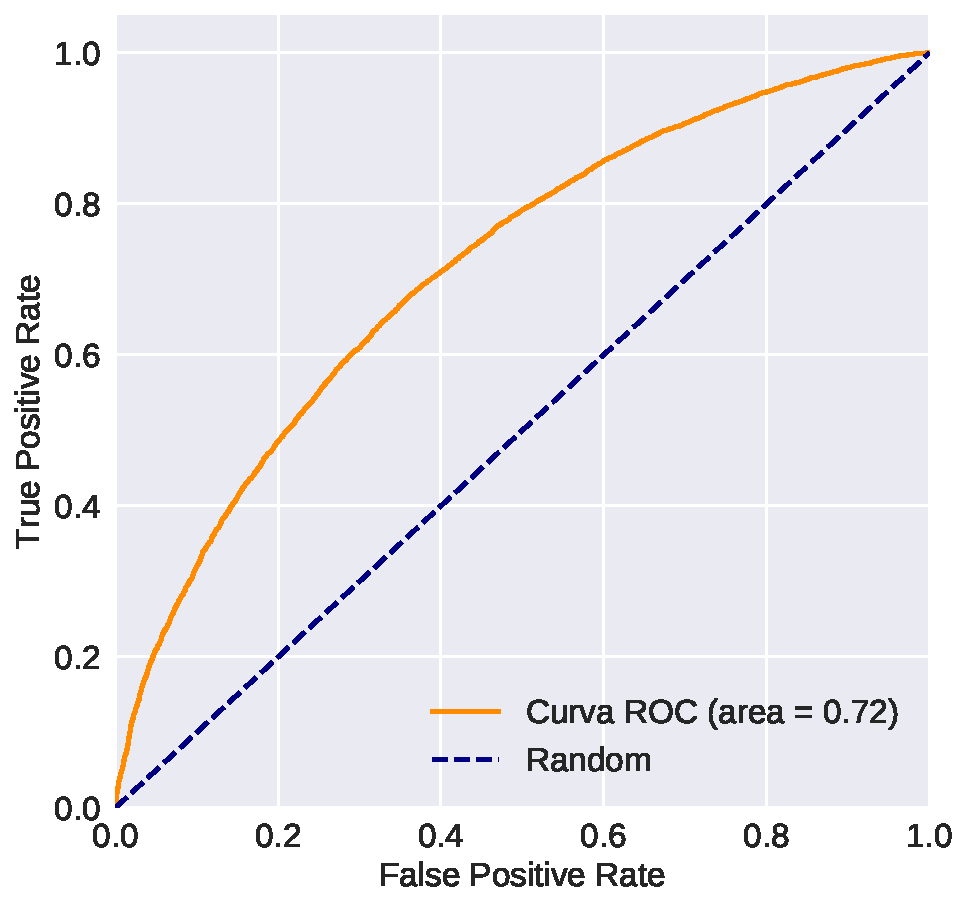
\includegraphics[width=\textwidth]{documents/latex/figures/3/structural/auc_structural.pdf}
    \caption{Curva AUC del modelo. La línea punteada corresponde a un predictor Random.}
    \label{fig:auc_structural}
\end{subfigure}

\hfill
\hfill

\begin{subfigure}[b]{0.7\textwidth}
    \centering
    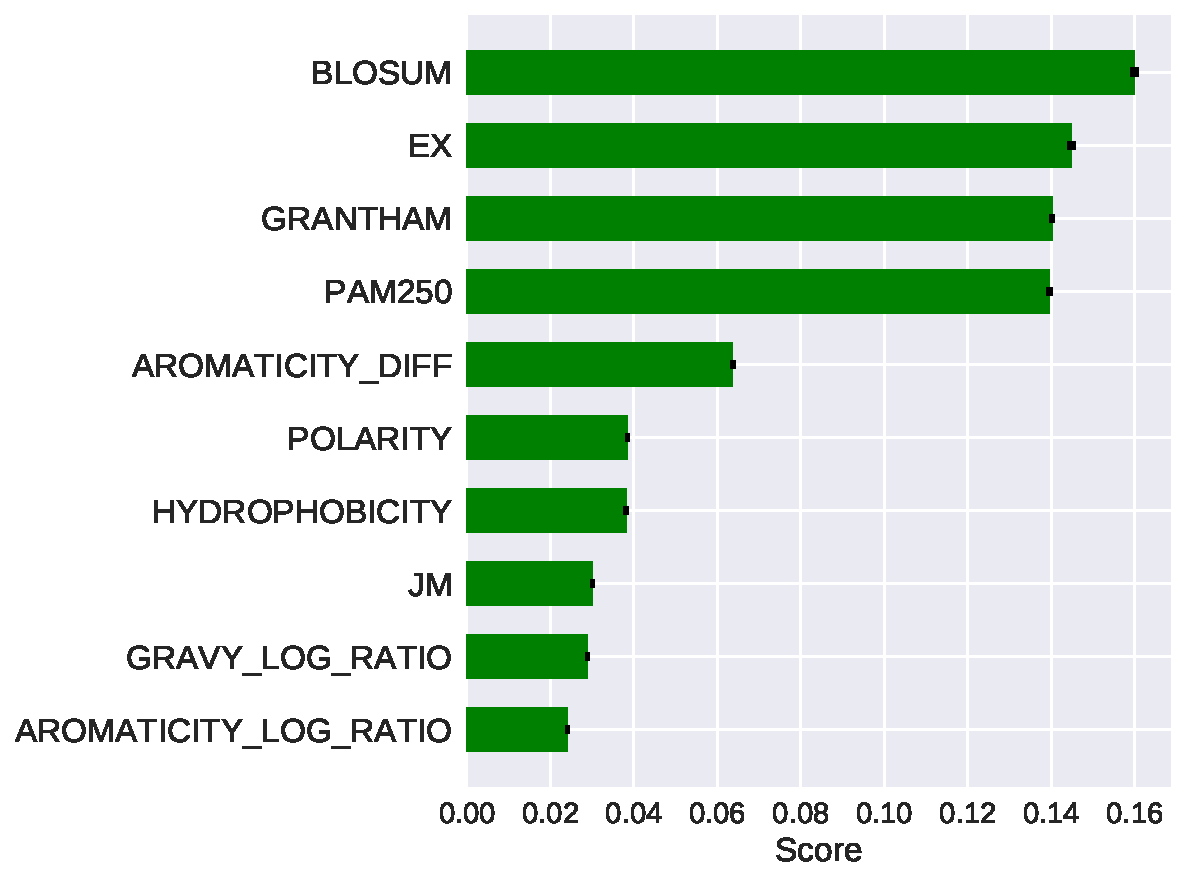
\includegraphics[width=\textwidth]{documents/latex/figures/3/structural/importances_structural.pdf}
    \caption{Los 10 atributos más importantes del modelo según el método estándar de \texttt{scikit-learn}.}
    \label{fig:importances_structural}
\end{subfigure}

\caption{Curva AUC y atributos más importantes del modelo Random Forest aplicado al dataset Físico-Químico. Hiperparámetros del modelo: Profundidad del árbol 7, 20\% de la cantidad de variables total en cada corte y 100 árboles.}
\end{figure}




\chapter{Modelo usando variables genómicas}
\label{ch:desarrollo_genomico}
% \section{Modelo usando variables genómicas}

Otra de las preguntas que nos hicimos fue si las variables genómicas podían hacer un aporte al modelo, siendo que es en los genes donde se produce la mutación que finalmente da origen a la variante en la proteína. En la base de datos Humsavar existe, para la mayoría de las mutaciones, el identificador rsID o Reference SNP ID. Un identificador rsID agrupa los distintos reportes que hacen referencia a la misma posición dentro del mismo genoma de referencia (hg19/GRCh37, en nuestro caso). A partir de este identificador fue posible obtener de la base de datos dbSNP (Versión snp150) \cite{dbSNP}, datos como el cromosoma, la posición, el cambio de nucleótido de la variante y su clasificación funcional.

\section{Variables de conservación}

En la literatura encontramos que dos de las variables genómicas asociadas a la conservación eran las que daban mejores resultados de predicción (modelos FATHMM-MKL \cite{Shihab2015} o VEST \cite{Carter2013}). La \textit{conservación} es un concepto biológico que refiere a las secuencias conservadas, es decir, secuencias tanto genéticas como proteicas que se mantienen de forma similar o idéntica en muchas especies que poseen un ancestro evolutivo en común. La conservación puede ser cuantificada con distintos tipos de enfoques, pero en lo que nos concierne, dos de los más utilizados son 1) a través de alineamientos múltiples de secuencias y 2), mediante el uso de árboles filogenéticos.

En particular, la composición de estas variables consiste en alineamientos múltiples de secuencias genéticas (MSA) de 46 especies de vertebrados, incluyendo Homo Sapiens y otras como Felis catus (gato doméstico), Danio renus (pez cebra) y Equus Caballus (caballo). En base a este alineamiento se usan dos medidas distintas que buscan detectar aquellas regiones en el genoma (ADN) con mayor nivel de conservación entre las distintas especies. Las medidas son las siguientes:
\begin{itemize}
    \item \textbf{PhastCons-46-Way} \cite{siepel2005evolutionarily}: Medida de conservación basado en un modelo oculto de Markov (\textit{phylo-HMM}). Calcula la probabilidad de que un nucleótido pertenezca a un sitio conservado (considerando el entorno).
    \item \textbf{PhyloP-46-Way} \cite{Pollard2010}: mide la conservación en una columna individual, sin considerar las columnas vecinas.
\end{itemize}

Decidimos incluir en nuestro dataset ambas medidas de conservación, usando el Table Browser de la Universidad de California en Santa Cruz (UCSC) \cite{Karolchik2004}.

\section{Variables relativas a la clase funcional}

También tomamos en consideración la función de la posición dentro del gen. La base de datos dbSNP define cada SNP de acuerdo a su clase funcional. Si la variación se encuentra cerca del intervalo de un transcripto, pero no en la región codificante, la clase funcional va a depender de la posición de la variación relativa a la estructura del transcripto \cite{Kitts2014}.  Por otro lado, si la variación se encuentra en una zona codificante, la clase funcional se va a definir en base a si el alelo de la variación va a resultar en una sustitución sinónima (es decir, el nuevo codón va a formar el mismo aminoácido), una sustitución \textit{missense} (es decir, el nuevo codón va a formar un aminoácido distinto) o una sustitución \textit{nonsense} (en donde la mutación genera un codón de terminación prematuro). En base a esta información generamos variables binarias, que indican con 1 ó 0 la existencia de un lugar con una determinada clase funcional.

Las categorías de clases funcionales que usamos en este caso fueron \cite{tablefuncclasses}:
 
\begin{itemize}
    \setlength\itemsep{0em}
    \item INTRON
    \item MISSENSE
    \item NEAR-GENE
    \item NCRNA
    \item CODING-SYNON
    \item UNTRANSLATED
    \item NONSENSE
    \item SPLICE
    \item STOP-LOSS
\end{itemize}

\section{Extracción de variables usando SNVBox}

Por último, usamos variables genómicas del dataset SNVBox, específicamente de la tabla \\ EXON\_FEATURES. Las variables usadas son:
\begin{itemize}
    \item ExonConservation (CONS): Score de Conservación para el exón completo calculado a partir de una alineación filogenética a 46 vías, usando el \textit{Genome Browser}. Si bien existe una gran similitud con las variables de conservación que ya incluimos en el dataset decidimos incluir esta variable debido a su baja correlación con las mencionadas anteriormente (ver descripción estadística del dataset más adelante).
    \item ExonHapMapSnpDensity (HAPMAP\_SNP\_DEN): Número de SNPs (verificados en HapMap) en el exón donde ocurre la mutación dividido por la longitud del exón. Estos SNPs (también llamados tag SNPs) son los que identifican haplotipos. Los haplotipos son bloques de SNPs heredados por un único individuo.
    \item ExonSnpDensity (SNP\_DEN): Número de SNPs en el exón donde ocurre la mutación dividido por la longitud del exón.
\end{itemize}

Estas variables se definen a nivel de exón, por lo que cada una de ellas posee dos identificadores: UID (identificador de la secuencia proteica a la que pertenece, propia de la base de datos) y EXON ID (identificador del exón dentro de cada transcripto mRNA). Estos identicadores permiten el cruce con la tabla \texttt{Transcript\_Exon} dentro de la base SNVBox. Con esta tabla podemos obtener el número del cromosoma del exón, y la posición de inicio y fin del exón dentro del cromosoma. Una vez obtenidos estos datos, pudimos extraer todos los rsID dentro de esa subsecuencia. Para aproximadamente el 33\% de los rsIDs en nuestra tabla Humsavar existe más de un transcripto que los contiene, por lo que decidimos promediar las variables (Cons, snp\_den y hapmap\_snp\_den) de cada uno de los transcriptos.

\begin{figure}[H]
\centering
    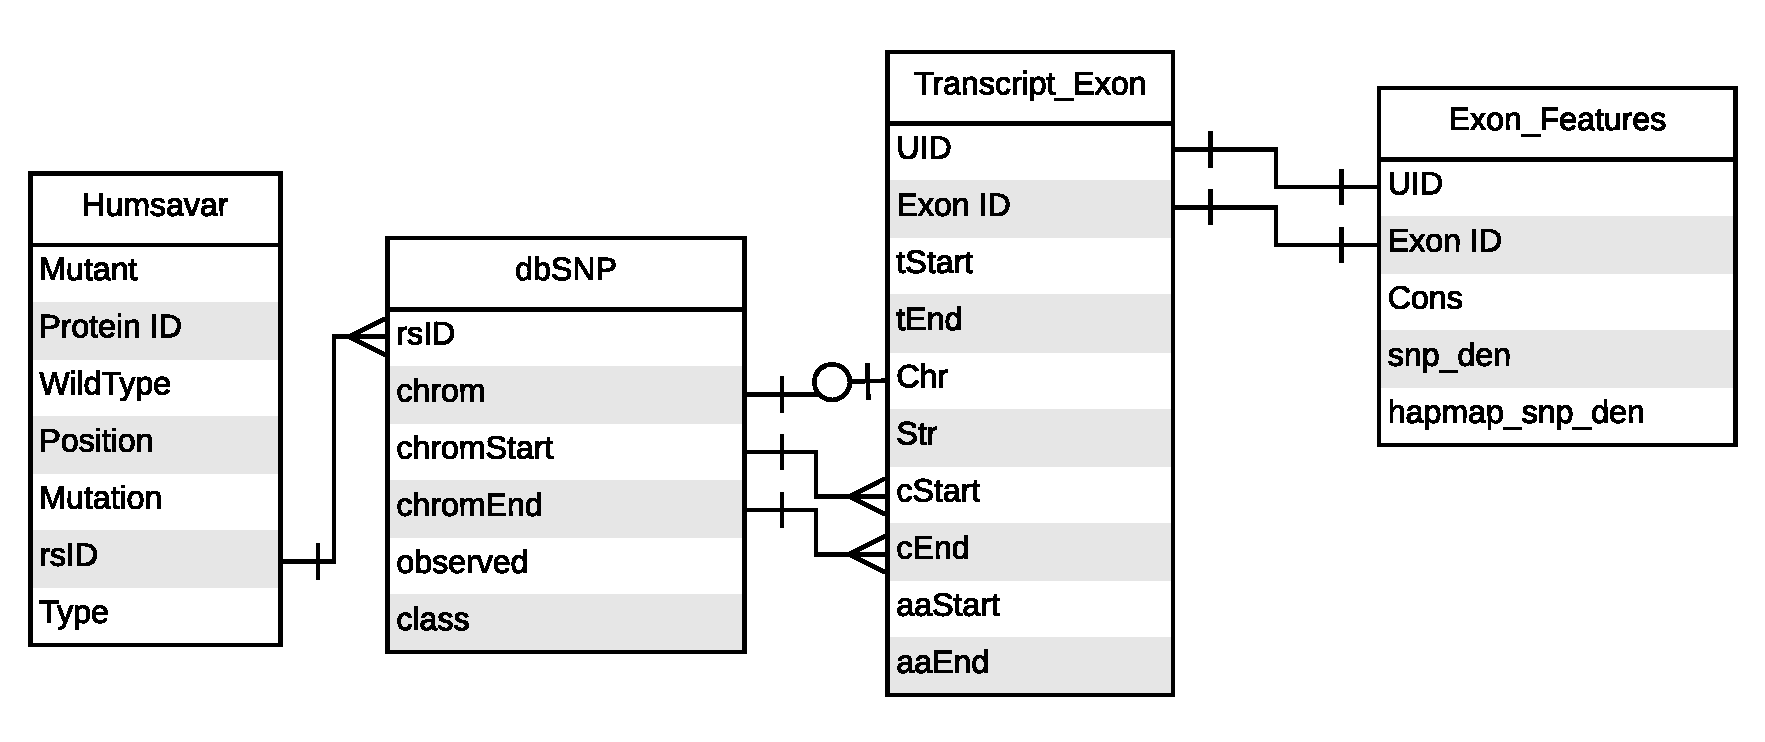
\includegraphics[scale=0.40]{documents/latex/figures/3/genomic/exon_diagram.pdf}
    \caption{Esquema de acceso a las variables genómicas de SNVBox.}
    \label{fig:exon_diagram}
\end{figure}

\section{Construcción del dataset Genómico}

Con los atributos mencionados anteriormente, pudimos cruzar la información usando la columna rsID (Reference SNP cluster ID). Esta columna identifica a un cluster de variaciones de un sólo nucleótido que pertenece a la misma posición en el genoma (o conjunto de posiciones) \cite{Ostell2007}. Filtramos las variantes de Humsavar que no poseían este identificador. Finalmente el dataset Genómico se compone de 55,382 variantes de las cuales 37,572 (68\%) son benignas y 17,807 (32\%) son patogénicas. 

\section{Descripción estadística del dataset Genómico}

A continuación presentamos, como en las secciones anteriores, una descripción de las variables usadas (ver tablas \ref{conservacion_vars} y \ref{snvbox_vars}). Para cada uno de los grupos analizamos la media (mean), el desvío estándar (std), los cuartiles (25\%, 50\%, 75\%) y los valores máximos (max) y mínimos (min). También calculamos el AUC univariado y el \textit{Balanced Accuracy} para las variables categóricas, en este caso las relativas a la clase funcional. El AUC univariado de las variables de conservación (PHYLOP46WAY, PHASTCONS46WAY y CONS) es alto, lo que significa que variantes en zonas de alta conservación son buenos indicadores de patogenicidad. En el caso de las variables categóricas del dataset (las variables relativas a la clase funcional), no encontramos variables con un BACC significativo.

% \subsection{Variables de Conservación}
\begin{table}[H]
\centering
\begin{tabular}{|l|l|l|l|l|l|l|l|l|}
\hline
Variable & mean & std & min & 25\%  & 50\% & 75\%  & max & AUC \\ \hline
PHYLOP46WAY & 2.16 &  2.29 & -8.22 &  0.29 &  1.81 &  4.23 &  6.42 & 0.83 \\ \hline
PHASTCONS46WAY & 0.67 & 0.44 &  0.00 &  0.06 &  0.99 &  1.00 &  1.00 & 0.78 \\ \hline
\end{tabular}
\caption{Variables de Conservación del dataset Genómico.}
\label{conservacion_vars}
\end{table}

% \subsection{}
\begin{table}[H]
\centering
\begin{tabular}{|l|l|l|l|l|l|l|l|l|}
\hline
Variable         & mean & std  & min  & 25\% & 50\% & 75\% & max & AUC  \\ \hline
CONS             & 0.65 & 0.09 & 0.14 & 0.59 & 0.66 & 0.72 & 0.90 & 0.65 \\ \hline
SNP\_DEN         & 0.06 & 0.10 & 0.00 & 0.03 & 0.04 & 0.06 & 1.04 & 0.56 \\ \hline
HAPMAP\_SNP\_DEN & 0.00 & 0.00 & 0.00 & 0.00 & 0.00 & 0.00 & 0.04 & 0.48 \\ \hline
\end{tabular}
\caption{Variables extraídas de SNVBox a nivel de Exón del dataset Genómico.}
\label{snvbox_vars}
\end{table}

% \subsection{Correlación entre las variables}

Con respecto a los valores nulos, tenemos una cobertura muy alta de todas las variables, con una porcentaje de nulos máximo del 2\%. (figura \ref{fig:proporcion_nulos_genomic}). 


% \newpage

\begin{figure}[H]
    \centering
    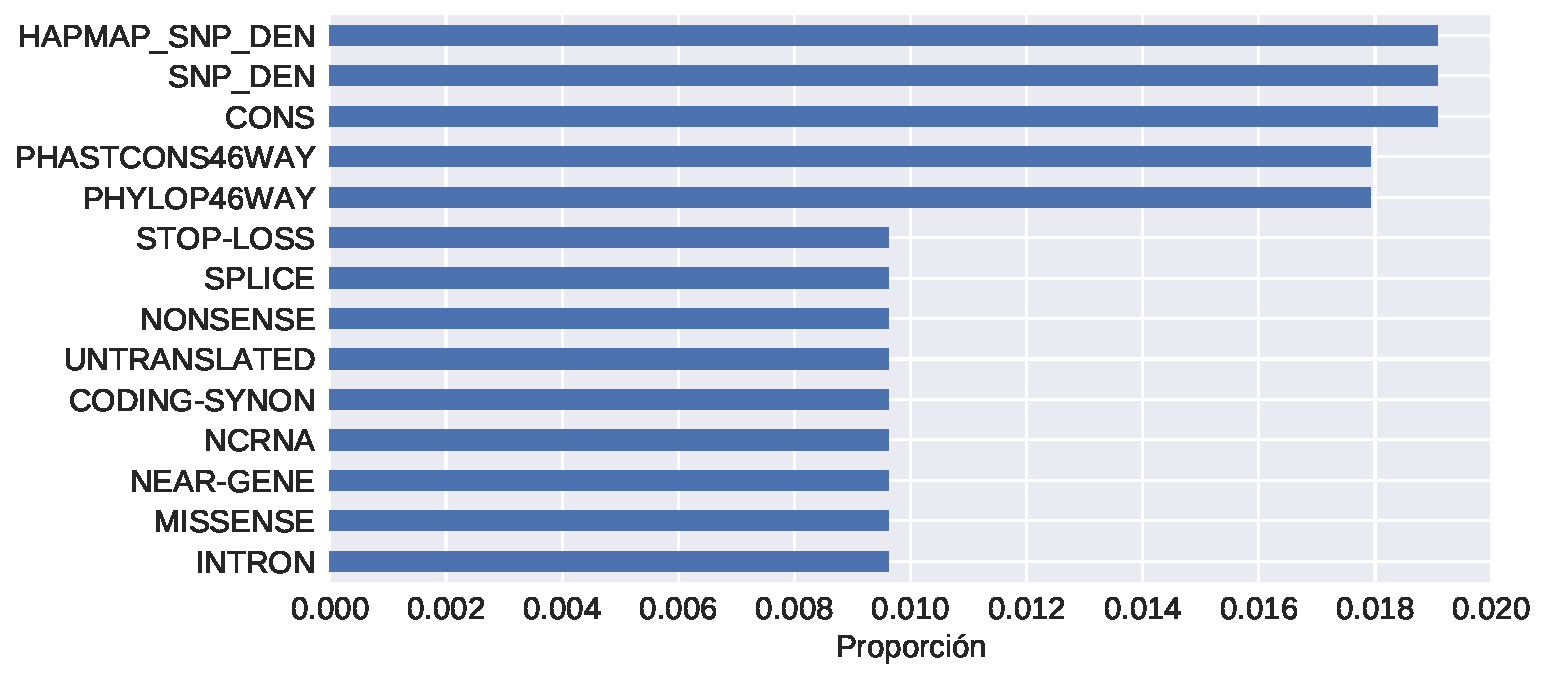
\includegraphics[scale=0.6]{documents/latex/figures/3/genomic/proporcion_nulos_genomic.pdf}
    \caption{Proporción de nulos del dataset Genómico.}
    \label{fig:proporcion_nulos_genomic}
\end{figure}

Como era de esperarse, la figura \ref{fig:corrplot_genomic} muestra una alta correlación de Spearman entre las variables de conservación PHYLOP46WAY y PHASTCONS46WAY (0.82). Por otro lado, la correlación entre HAPMAP\_SNP\_DEN y SNP\_DEN es muy baja (0.06), pese a que su construcción es muy similar. Esto se debe a la diferencia entre la cantidad total de SNPs en un humano (alrededor de 10 millones) comparados con los que se encuentran en HapMap (aproximadamente 500,000 en total).

\begin{figure}[H]
    \centering
    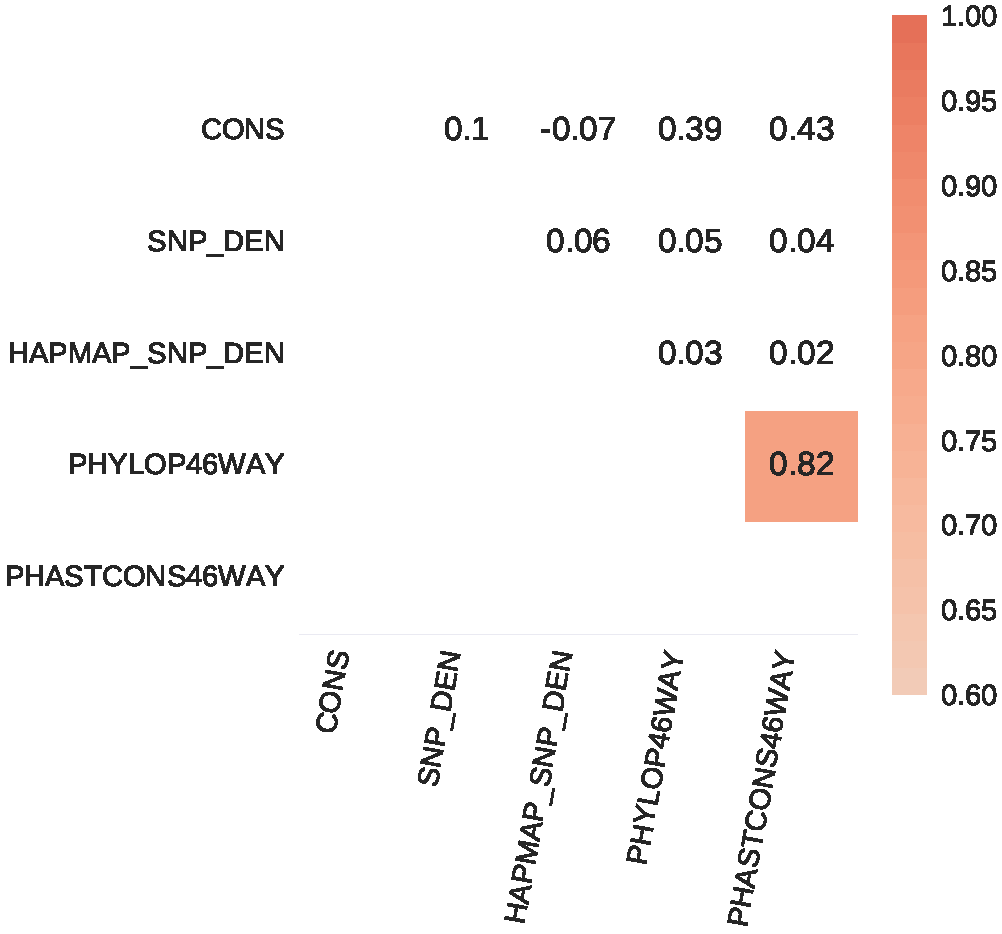
\includegraphics[scale=0.5]{documents/latex/figures/3/genomic/genomic_corr.pdf}
    \caption{Correlación de Spearman para las variables continuas del dataset Genómico.}
    \label{fig:corrplot_genomic}
\end{figure}

% \newpage

\section{Generación del modelo}

Luego de realizada la exploración del dataset Genómico generamos un modelo basado en Random Forest. Volvimos a utilizar este algoritmo debido a los resultados obtenidos en el dataset VarQ Curado y para facilitar la comparación entre los datasets estudiados. Volvimos a utilizar el Pipeline Tree del capítulo anterior. Nuevamente, las variables no fueron escaladas dado que en los algoritmos que involucran árboles de decisión, como Random Forest, las variables son evaluadas una a una y por lo tanto la escala de cada una de ellas no afecta la evaluación de las demás.

\section{Resultados del modelo Genómico}

Como se puede observar en la figura \ref{fig:auc_genomic} obtuvimos un AUC de 0.85. Los hiperparámetros escogidos en la fase de entrenamiento fueron una profundidad del árbol máxima de 7, una cantidad máxima de variables de 7 y un 100 estimadores.
Este resultado es muy superior a los obtenidos en los modelos anteriores, tanto en VarQ Curado como en el dataset Físico-Químico. En la tabla \ref{tab:metrics_genomic} vemos los valores de \textit{precision}, \textit{recall} y \textit{f1-score} para las dos clases. En este caso podemos advertir una mejora total en cada una de las métricas comparándolas con las obtenidas en base al modelo Físico-Químico. En particular destacamos la mejora en precisión de la detección de variables benignas, que pasó de un 0.68 en el modelo Físico-Químico a un 0.83 en el modelo Genómico, es decir un 15\% de mejora; como así también el crecimiento en el \textit{recall} de variantes patogénicas, que saltó de un 0.47 en el modelo Físico-Químico a un 0.64, lo que representa un 17\% de mejora.

\begin{table}[H]
\centering
\begin{tabular}{|l|l|l|l|}
\hline
             & Precisión & Recall & F1-score \\ \hline
Benignas     & 0.83      & 0.87   & 0.85     \\ \hline
Patogénicas  & 0.69      & 0.64   & 0.67     \\ \hline
Promedio     & 0.79      & 0.79   & 0.79     \\ \hline
\end{tabular}
\caption{Reporte de métricas del modelo Random Forest usando el dataset Genómico.}
\label{tab:metrics_genomic}
\end{table}

% Otra de las razones que explican esta diferencia es la forma en que son calculadas. El dataset VarQ usa una variable basada a nivel de proteínas 


\section{Importancia de los atributos}
Analizando la importancia de las variables en el modelo, en la figura \ref{fig:importances_genomic} podemos observar que las variables de conservación (PHYLOP46WAY y PHASTCONS46WAY) están en los primeros dos puestos, confirmando lo obtenido por los trabajos de investigación antes mencionados \cite{Shihab2015} \cite{Carter2013}. 

El poder informativo sumado de estas variables equivale a un porcentaje superior al 80\% de la importancia total. La pregunta que nos hacemos en este caso es: ¿Las dos primeras variables de conservación están en los primeros dos lugares porque están altamente correlacionadas o aportan diferente información sobre las variables? En base al análisis de correlación de Spearman (ver figura 2.12), podemos observar que estas variables se encuentran muy correlacionadas (0.82), lo que sugiere un alto grado de redundancia. En la figura \ref{fig:importance_genomic_cluster}, observamos que esta proporción se mantiene al agrupar en clusters a las variables correlacionadas.

Por otro lado, esto genera un interrogante adicional: ¿Cuál es la razón por la que la variable \textit{Conservación} del dataset VarQ Curado no genera un rendimiento similar? Una de las principales razones que encontramos es en el nivel de cobertura de la variable. En el caso de las variables de conservación genómica, la cobertura de las mismas llega a un nivel superior al 95\%, mientras que en el caso de la conservación en el dataset VarQ Curado este número no llega al 40\%. La cobertura de estas variables posee aproximadamente la misma proporción para variables patogénicas y benignas que la proporción original en ambos datasets. Otra razón posible a considerar tiene que ver con la naturaleza del cálculo de conservación de VarQ via PFAM, que contiene una heterogeneidad muy grande de especies (alrededor de 16,000 familias), y se basa en secuencias de proteínas, mientras que PHYLOP46WAY y PHASTCONS46WAY se basa en secuencias genómicas.

\begin{figure}[H]
    \centering
    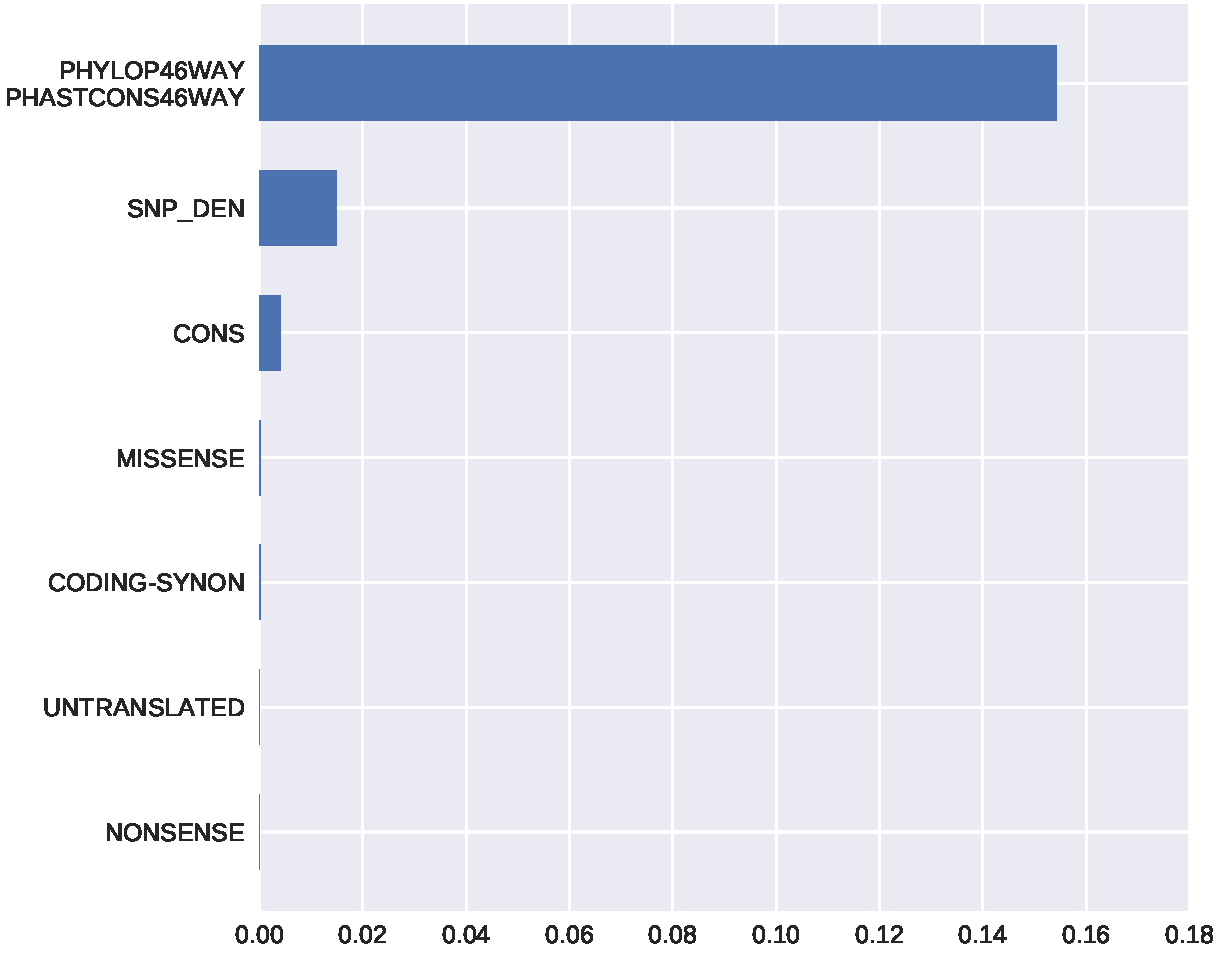
\includegraphics[scale=0.7]{documents/latex/figures/3/genomic/genomic_importance_cluster.pdf}
    \caption{Variación en la precisión al permutar clusters de variables correlacionadas ($>$ 0.90) del dataset Genómico.}
    \label{fig:importance_genomic_cluster}
\end{figure}


\newpage

\begin{figure}[H]
\centering
\begin{subfigure}[b]{0.7\textwidth}
    \centering
    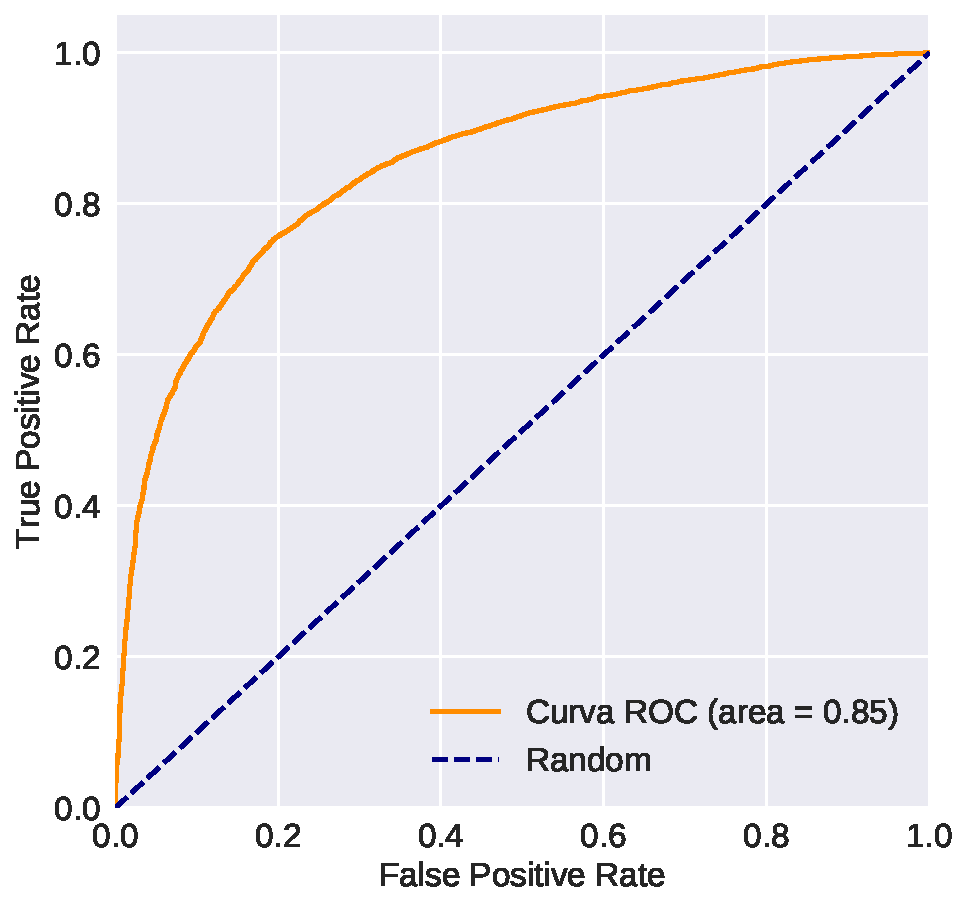
\includegraphics[width=\textwidth]{documents/latex/figures/3/genomic/auc_genomic.pdf}
    \caption{Curva AUC del modelo. La línea punteada corresponde a un predictor Random.}
    \label{fig:auc_genomic}
\end{subfigure}

\hfill
\hfill

\begin{subfigure}[b]{0.7\textwidth}
    \centering
    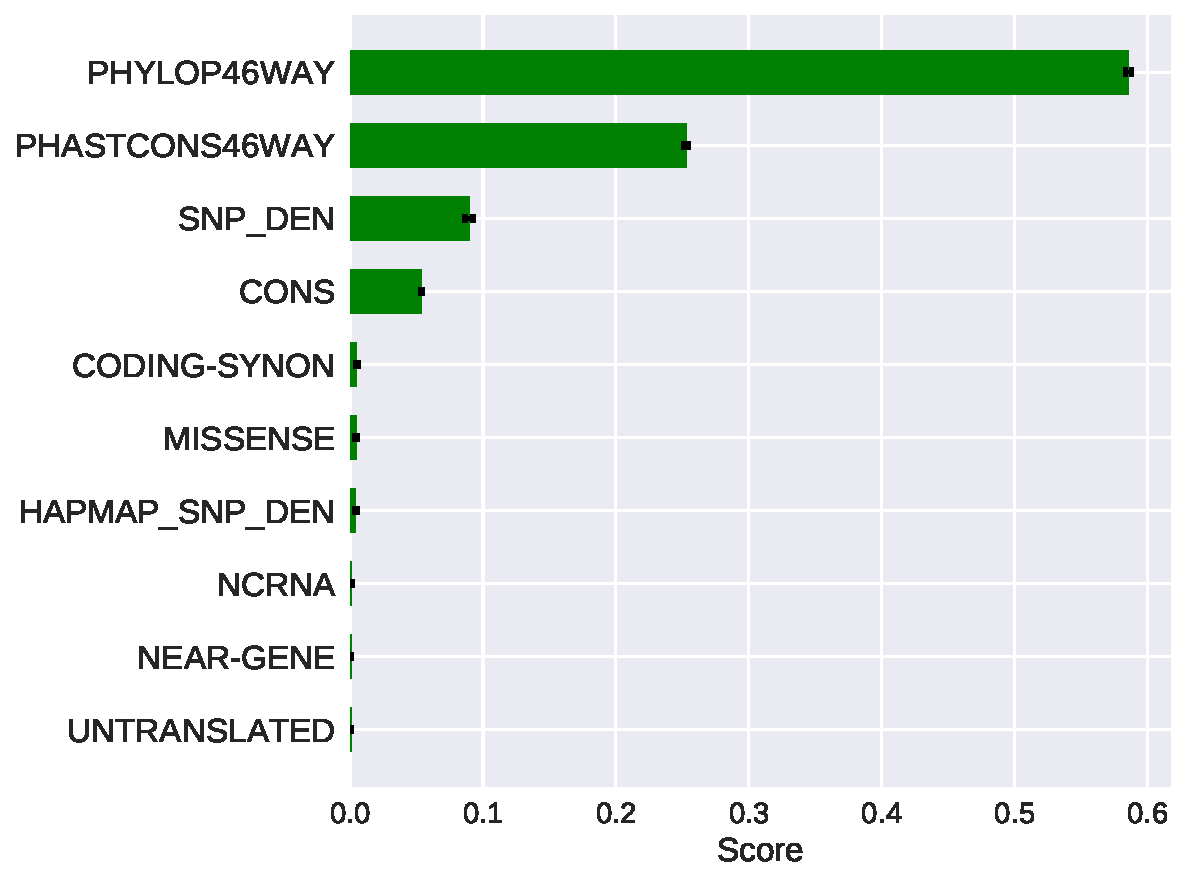
\includegraphics[width=\textwidth]{documents/latex/figures/3/genomic/importances_genomic.pdf}
    \caption{Los 10 atributos más importantes del modelo.}
    \label{fig:importances_genomic}
\end{subfigure}

\caption{Curva AUC y atributos más importantes del modelo Random Forest aplicado al dataset Genómico. Hiperparámetros del modelo: Profundidad del árbol 7, 7 variables en cada corte y 100 árboles.}

\end{figure}


\chapter{Integrando el dataset Físico-Químico y el Genómico}
\label{ch:desarrollo_integral}
% \section{Integrando el dataset Físico-Químico y el Genómico}

En este capítulo unimos los dos conjuntos de variables para evaluar si la integración de ambos datasets representan una mejora frente a los resultados de los modelos Genómico y Físico-Químico por separado. A este nuevo dataset lo denominamos dataset Integral. Las variantes usadas fueron nuevamente las encontradas en la tabla Humsavar. 

\section{Creación del dataset Integral}

El dataset Integral posee 68,508 variantes. Este número equivale a la cantidad de variantes del dataset Físico-Químico, y esto se debe a que conservamos todas sus variantes sumando variables del Dataset Genómico (ver figura \ref{fig:interseccion_integral}). Esto da un total de 64 variables, que son las variables sumadas de los datasets Genómico (14), Físico-Químico (49) y la variable de respuesta.  

\begin{figure}[H]
    \centering
    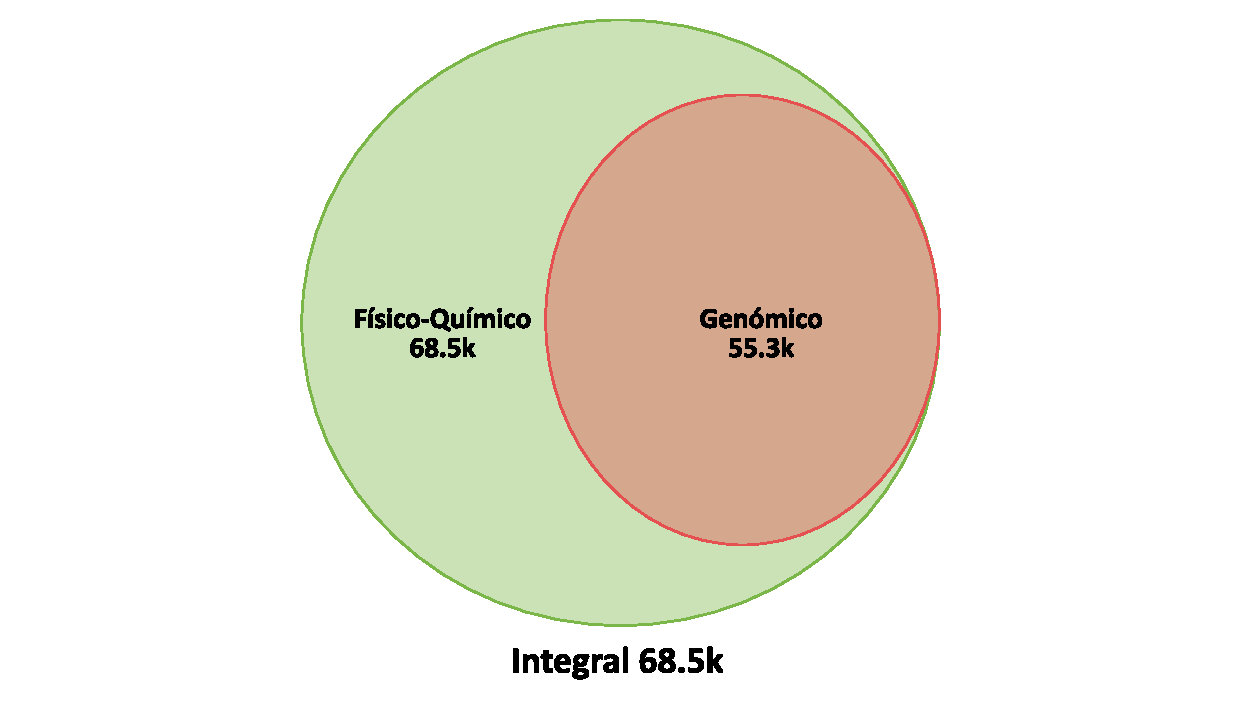
\includegraphics[scale=0.6]{documents/latex/figures/3/integral/interseccion_integral.pdf}
    \caption{Intersección entre los datasets Genómico y Físico-Químico.}
    \label{fig:interseccion_integral}
\end{figure}

Del total de las variantes, 39,653 (58\%) son benignas y 28,855 (42\%) son patogénicas. Con respecto a los nulos, mantenemos la misma cobertura de las variables físico-químicas del dataset homónimo (aproximadamente 35\% para las variables categóricas y una cobertura mayor del 60\% para las continuas), mientras que para las variables genómicas tenemos alrededor de un 20\% de variantes que no poseen cobertura al no tener un identificador rsID.

\section{Generación del modelo}

\subsection{Random Forest}

Para este modelo preliminar utilizamos nuevamente el Pipeline Tree, repitiendo las mismas fases de imputación y entrenamiento usadas previamente en los modelos Genómico y Físico-Químico. Esto significa que en la fase de imputación usamos la mediana para los valores nulos de las variables continuas y el valor más frecuente en las variables categóricas. El entrenamiento consistió en una búsqueda de hiperparámetros óptimos usando \textit{GridSearch} en un diccionario de posibles parámetros (ver sección 7.3 del apéndice), evaluados en una triple validación cruzada basándonos en el AUC como métrica a optimizar. El dataset de entrenamiento posee 45,900 variantes, aproximadamente dos tercios del dataset completo. Una vez entrenado el modelo usando este \textit{pipeline}, se evaluaron las variantes del dataset de testeo, es decir, el tercio restante del dataset completo. 

\subsection{XGBoost}

Posteriormente introducimos un método de boosting, XGBoost, nuevamente usando el Pipeline Tree. Los hiperparámetros de este método fueron elegidos usando una búsqueda randomizada (\textit{Randomized Grid-Search}). Este método de optimización fue elegido dado que las combinaciones que se evalúan en el método Grid Search son demasiadas (ver sección 7.3 del apéndice para diccionario completo de hiperparámetros explorados). La búsqueda randomizada evalúa las mismas alternativas pero eligiendo combinaciones de forma aleatoria, sin probar todas las combinaciones. También es posible evaluar valores tomados de acuerdo a una distribución específica. Decidimos dejar este análisis para trabajos futuros.

\section{Resultados del modelo Integral}

\subsection{Modelo usando Random Forest}

El modelo Random Forest obtuvo un AUC de 0.88 (ver figura \ref{fig:auc_integral}). Esto representa una mejora con respecto al modelo Genómico (0.85) y al modelo Físico-Químico (0.72). Los hiperparámetros escogidos fueron: profundidad del árbol 7 (\texttt{max\_depth}), una cantidad máxima de variables del 20\% de las variables predictoras (\texttt{max\_features}) y 100 árboles (\texttt{n\_estimators}).
Si comparamos las métricas obtenidas en el modelo Genómico con las de este modelo (ver tabla \ref{tab:metrics_integral_rf}), se puede apreciar un nuevo salto en el Recall de las variables patogénicas, que pasa de un 0.64 en el modelo Genómico al 0.80, lo que representa un 25\% de mejora. También mejora la precisión con respecto a la detección de esta clase, que pasa de 0.69 a 0.76. La única métrica que decae es el Recall de la clase Benigna, que pasa de 0.87 a 0.82, lo que representa una leve caída del F1-score. 

\begin{table}[H]
\centering
\begin{tabular}{|l|l|l|l|}
\hline
Clase        & Precisión & Recall & F1-score \\ \hline
Benignas     & 0.85      & 0.82   & 0.83     \\ \hline
Patogénicas  & 0.76      & 0.80   & 0.78     \\ \hline
Promedio     & 0.81      & 0.81   & 0.81     \\ \hline
\end{tabular}
\caption{Reporte de métricas del modelo Random Forest usando el dataset Integral.}
\label{tab:metrics_integral_rf}
\end{table}


\subsection{Modelo usando XGBoost}

El modelo XGBoost superó la performance de Random Forest alcanzando un AUC de 0.90. Las otras métricas (Precisión, Recall, F1-score) también fueron levemente superiores en todos los casos, tanto para variables benignas como patogénicas (ver tabla \ref{tab:metrics_integral_xgb}). Los hiperparámetros obtenidos en el \textit{Randomized Grid-Search} fueron:

\begin{itemize}
    \item \texttt{min\_child\_weight}: 5
    \item \texttt{gamma}: 5
    \item \texttt{subsample}: 0.8
    \item \texttt{colsample\_bytree}: 0.8
    \item \texttt{max\_depth}: 5
\end{itemize}

Utilizando el test de DeLong para comparar los AUCs del modelo RF y XGB obtuvimos un p-valor igual a $2\mathrm{e}{-16}$. Esto indica que las diferencias observadas en los valores de AUC pueden deberse a fluctuaciones aleatorias con probabilidad menor a $2\mathrm{e}{-16}$.

\begin{table}[H]
\centering
\begin{tabular}{|l|l|l|l|}
\hline
Clase        & Precisión & Recall & F1-score \\ \hline
Benignas     & 0.86      & 0.83   & 0.84     \\ \hline
Patogénicas  & 0.78      & 0.82   & 0.80     \\ \hline
Promedio     & 0.83      & 0.82   & 0.82     \\ \hline
\end{tabular}
\caption{Reporte de métricas del modelo XGB usando el dataset Integral.}
\label{tab:metrics_integral_xgb}
\end{table}

\subsection{Comparación entre los modelos}

En la tabla \ref{tab:metrics_model_integral} comparamos la Precisión, el Recall y el AUC, los tiempos de entrenamiento y de evaluación. Los tiempos de entrenamiento incluyen todas las variantes del set de entrenamiento, usando 3 folds en la etapa de validación y la búsqueda de hiperparámetros. El tiempo de evaluación equivale al tiempo de todas las variables del set de evaluación. Las métricas están basadas en las variantes patogénicas como variantes positivas. El modelo XGB supera al modelo RF en casi todas las métricas exceptuando al tiempo de entrenamiento, que incluso usando el método de busca de hiperparámetros randomizado resultó ser mucho más lento que el modelo RF, si bien es posible reducir aún más el espacio de búsqueda. Esto se debe mayormente a que a diferencia de RF que genera estimadores de forma paralela, XGB es iterativo, lo que ralentiza el proceso. 

\begin{table}[H]
\centering
\begin{tabular}{|l|l|l|l|l|l|l|}
\hline
Modelo & Precisión & Recall & AUC & F1-score & $t_{fit}$ & $t_{pred}$ \\ \hline
RF & 0.76 & 0.80 & 0.88 & 0.78 & 2m 2 s & 0.3 s \\ \hline
XGB & 0.78 & 0.82 & 0.90 & 0.80 & 12m 47s & 1.14 s \\ \hline
\end{tabular}
\caption{Comparación de métricas de modelos usando el dataset Integral. Las variables $t_{fit}$ y $t_{pred}$ corresponden al tiempo de entrenamiento y de predicción de todas las variantes}
\label{tab:metrics_model_integral}
\end{table}

\section{Importancia de las variables}

Al combinar los dos datasets Genómico y Físico-Químico volvimos a evaluar la importancia de las variables en los modelos, dado que las nuevas interacciones entre ellas pueden haber modificado los resultados anteriores. 

Si analizamos solamente la importancia usando el método de \texttt{scikit-learn} para el modelo RF (ver figura \ref{fig:importances_integral_rf}), nuevamente encontramos en primer lugar a las variables de conservación genómicas (PHYLOP46WAY y PHASTCONS46WAY), resultado esperable dado su nivel de importancia en el dataset Genómico y su nivel de AUC conseguido. También encontramos en un segundo escalón a las variables de conservación a nivel de exones, y a una variable que considera el número de SNPs en el exón donde ocurre la mutación. Luego encontramos al grupo de matrices de sustitución de aminoácidos (EX, GRANTHAM, BLOSUM y PAM250), que también aparecieron en los primeros lugares en el modelo Físico-Químico. Por último encontramos una variable relativa a la clase funcional a nivel genómico (MISSENSE) y otra relativa al cambio de polaridad del aminoácido donde ocurre la variante (POLARITY) y a la hidrofobicidad del aminoácido (HYDROPHOBICITY), por lo que encontramos en nuestro ranking una lista de variables transversal a los dos datasets usados. 


En las figuras \ref{fig:importance_cluster_integral_rf} y \ref{fig:importance_cluster_integral_xgb} unimos las variables de alta correlación en clusters y comparamos su impacto en la precisión del modelo usando la herramienta \texttt{rfpimp}. Notamos que la importancia de CONS se ve disminuida en el modelo XGB con respecto al modelo RF.


% \begin{figure}[H]
%     \centering
%     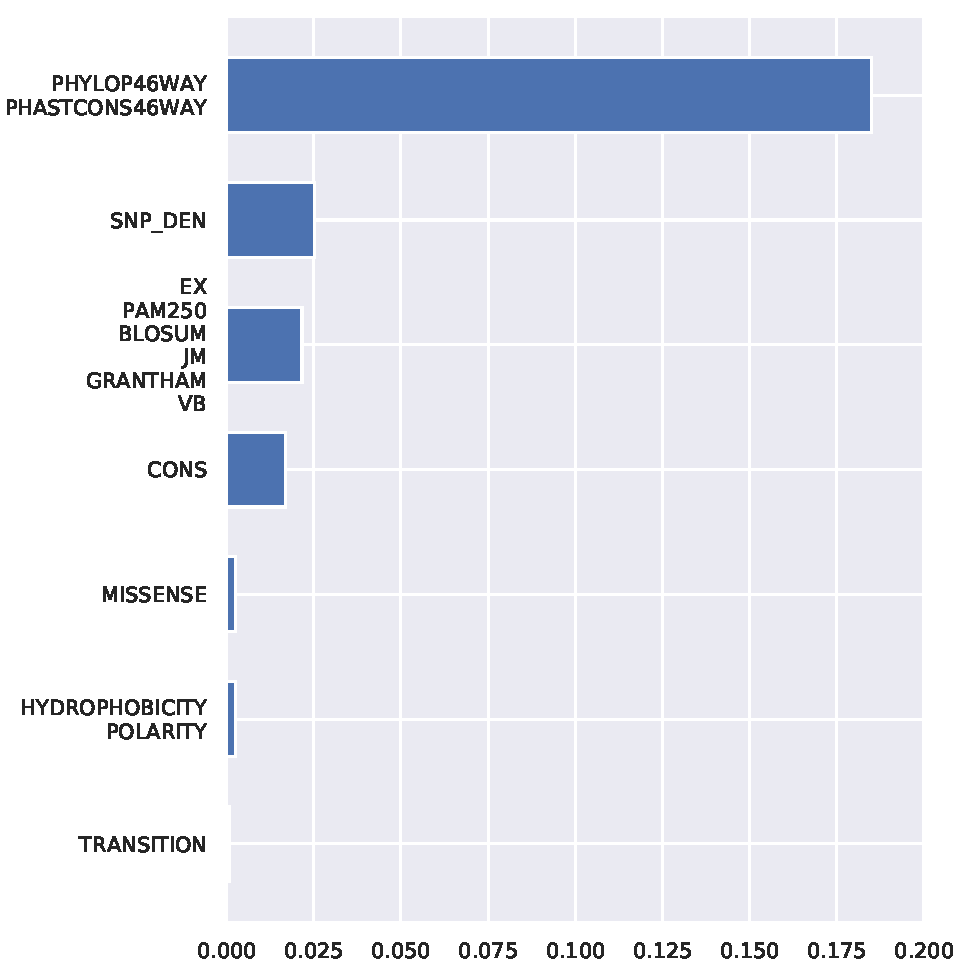
\includegraphics[scale=0.6]{documents/latex/figures/3/integral/integral_importance_cluster.pdf}
%     \caption{Importancia de variables altamente correlacionadas (basados en correlación de Spearman) usando permutación. Resultados del modelo usando Random Forest.}
%     \label{fig:importance_cluster_integral_rf}
% \end{figure}



% \begin{figure}[H]
%     \centering
%     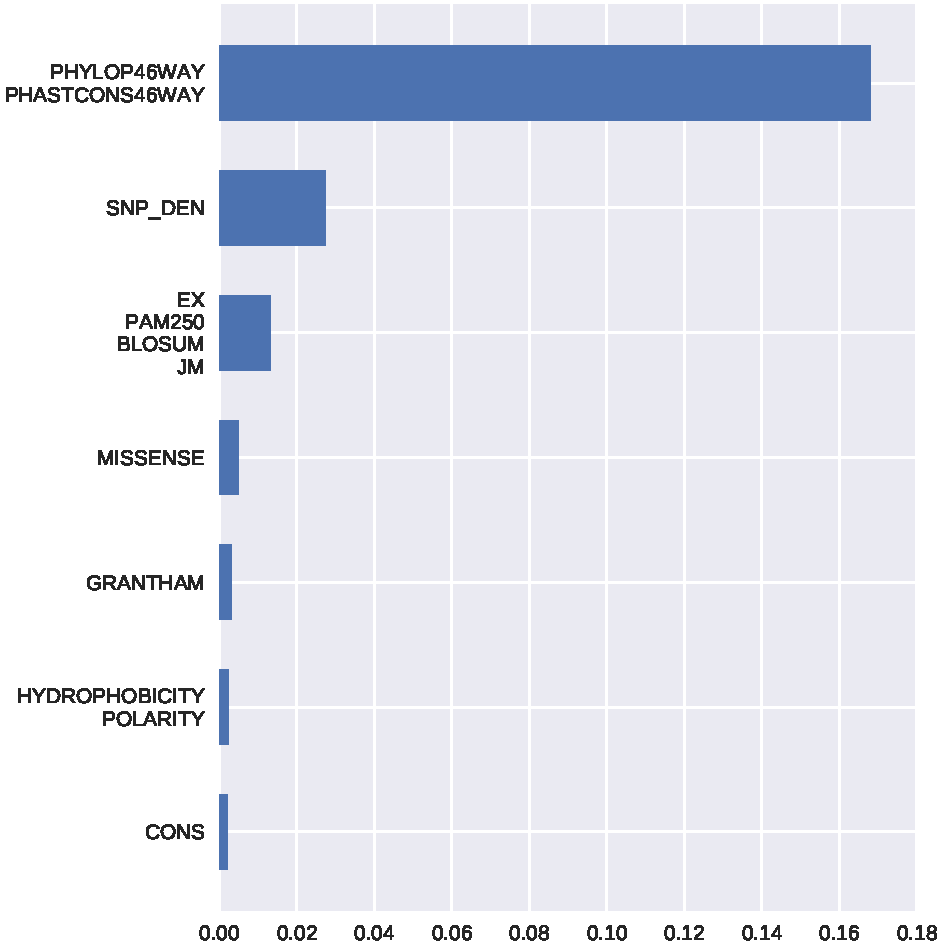
\includegraphics[scale=0.6]{documents/latex/figures/3/integral/integral_importance_cluster_xgb.pdf}
%     \caption{Importancia de variables altamente correlacionadas (basados en correlación de Spearman) usando permutación. Resultados del modelo usando XGB.}
%     \label{fig:importance_cluster_integral_xgb}
% \end{figure}

% Side by side figures 
\begin{figure}[H]
\begin{subfigure}[c]{0.45\linewidth}
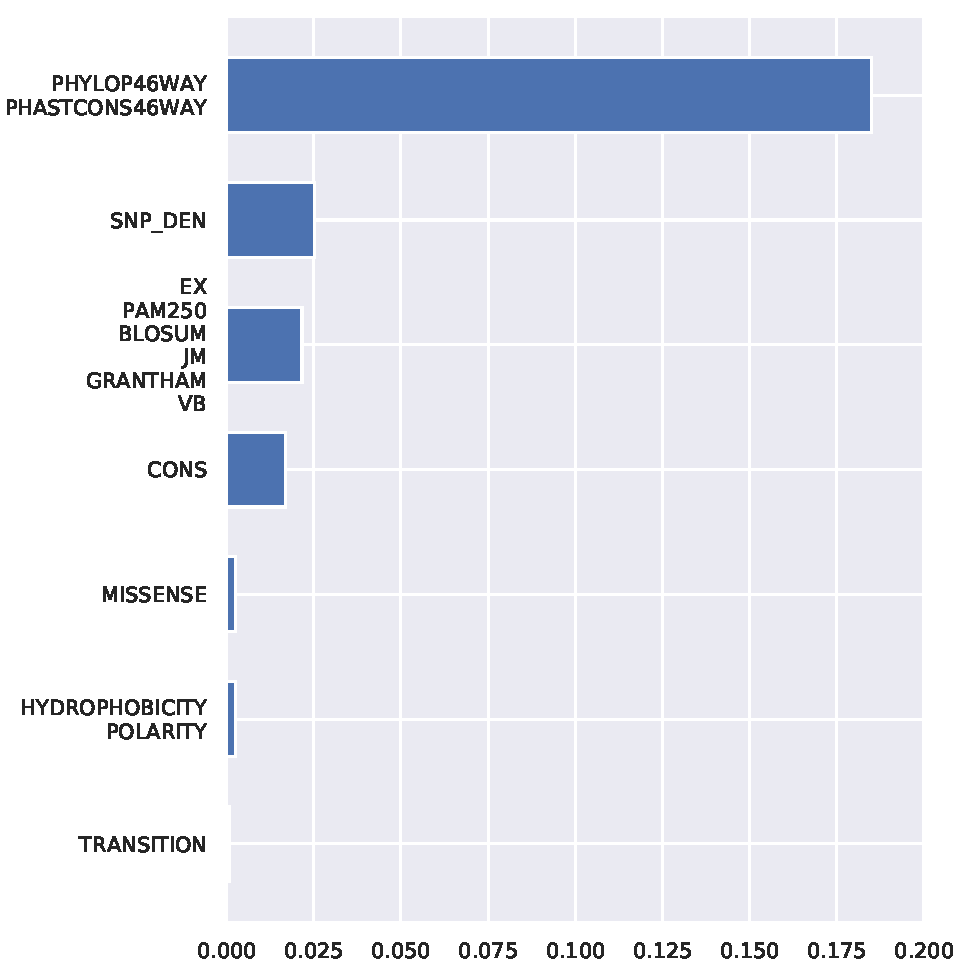
\includegraphics[width=\linewidth]{documents/latex/figures/3/integral/integral_importance_cluster.pdf}
\caption{Resultados del modelo usando RF.}
\label{fig:importance_cluster_integral_rf}
\end{subfigure}
% \hfill
\begin{subfigure}[c]{0.45\linewidth}
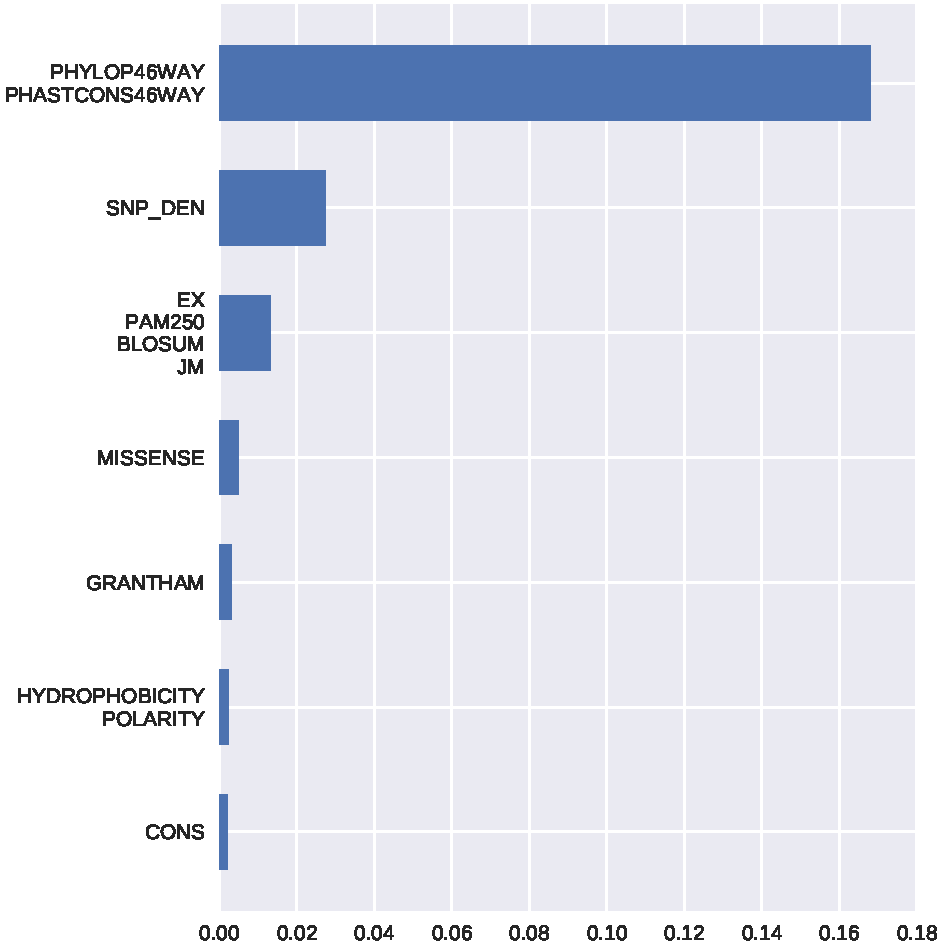
\includegraphics[width=\linewidth]{documents/latex/figures/3/integral/integral_importance_cluster_xgb.pdf}
\caption{Resultados del modelo usando XGB.}
\label{fig:importance_cluster_integral_xgb}
\end{subfigure}%
\caption{Importancia de variables altamente correlacionadas del dataset Integral (basados en correlación de Spearman) usando permutación.}
\end{figure}

\section{Conclusión del capítulo}

Como conclusión de este capítulo, resaltamos la mejora aportada tanto por el dataset Físico-Químico como por el algoritmo XGBoost. Por un lado, mantuvimos constante el algoritmo usado en la sección anterior, Random Forest, al que incluimos nuevas variables, y eso significó un salto en el AUC de 0.85 a 0.88. En un segundo paso, modificamos el algoritmo manteniendo las mismas variables, consiguiendo un AUC de 0.90. Consideramos que igualmente hay espacio para mejorar aún más, y evaluaremos la incorporación de variables estructurales en el próximo capítulo siguiendo el mismo esquema. 


% \begin{figure}[H]
% \begin{subfigure}[b]{0.5\textwidth}
%     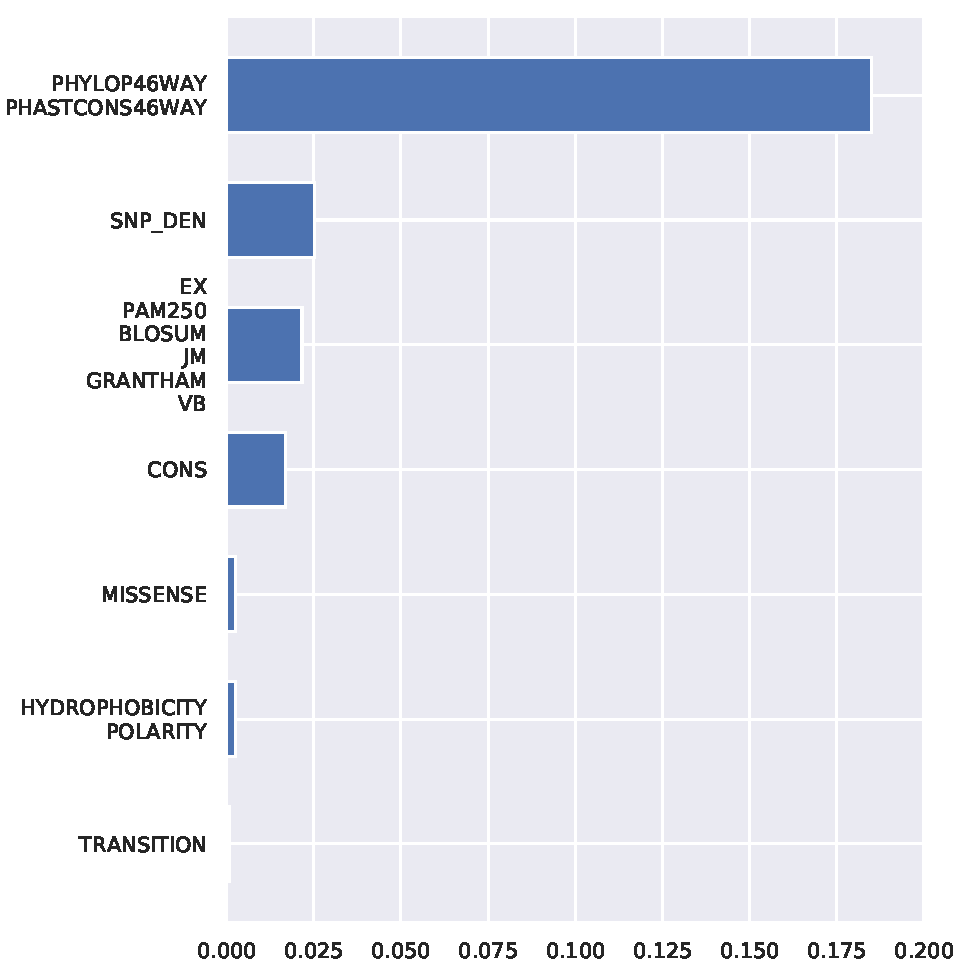
\includegraphics[width=\textwidth]{documents/latex/figures/3/integral/integral_importance_cluster.pdf}
%     \caption{Importancia de variables clusterizadas (basados en correlación de Spearman) usando permutación. Resultados del modelo usando Random Forest.}
%     \label{fig:importance_cluster_integral_rf}
% \end{subfigure}
% \hfill
% \hfill
% \begin{subfigure}[b]{0.5\textwidth}
%     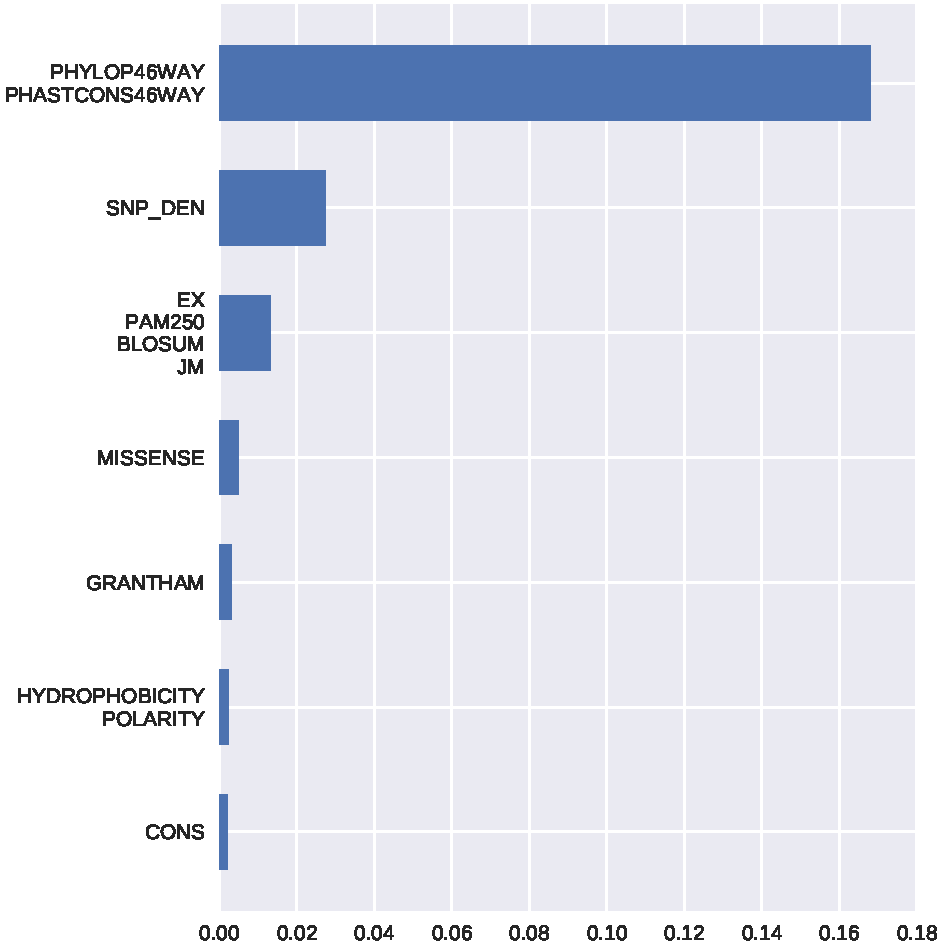
\includegraphics[width=\textwidth]{documents/latex/figures/3/integral/integral_importance_cluster_xgb.pdf}
%     \caption{Importancia de variables clusterizadas (basados en correlación de Spearman) usando permutación. Resultados del modelo usando XGB.}
%     \label{fig:importance_cluster_integral_xgb}
% \end{subfigure}

% \end{figure}





\newpage

\begin{figure}[H]
\centering
\begin{subfigure}[t]{0.7\textwidth}
    \centering
    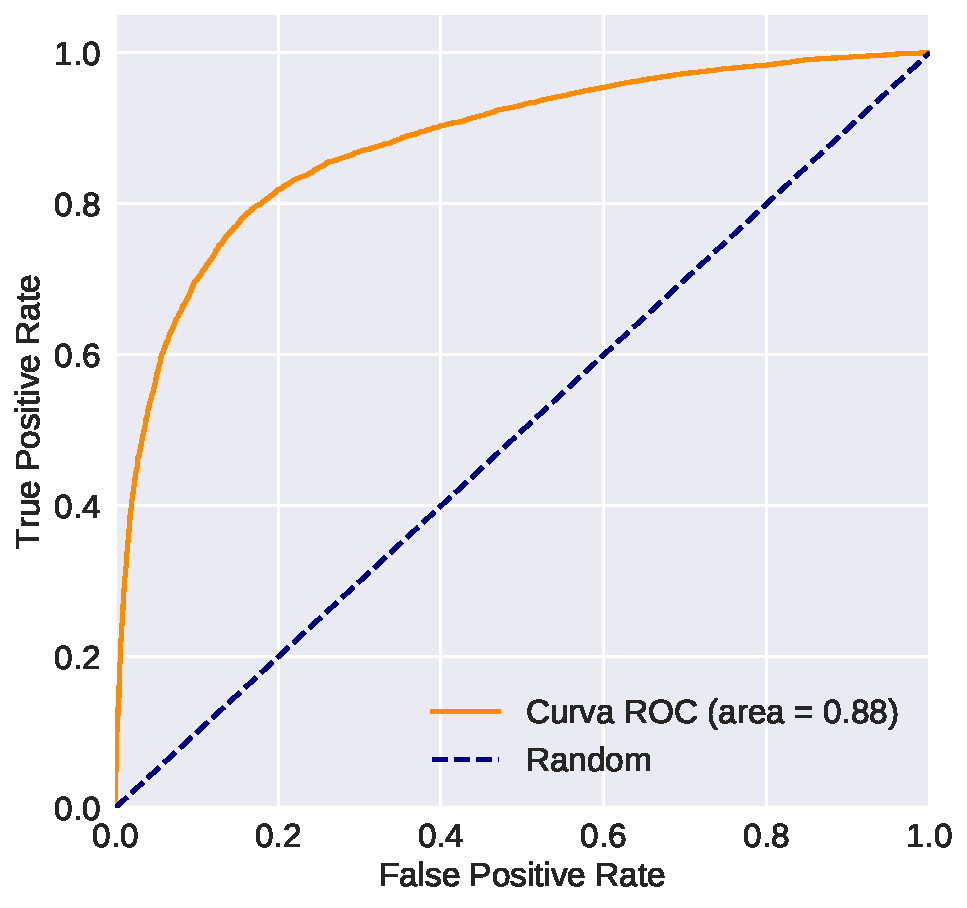
\includegraphics[width=\textwidth]{documents/latex/figures/3/integral/auc_integral.pdf}
    \caption{Comparación de curvas AUC entre algoritmos Random Forest y XGBoost. La línea punteada corresponde a un predictor Random.}
    \label{fig:auc_integral}
\end{subfigure}
\hfill
\hfill
\begin{subfigure}[b]{0.7\textwidth}
    \centering
    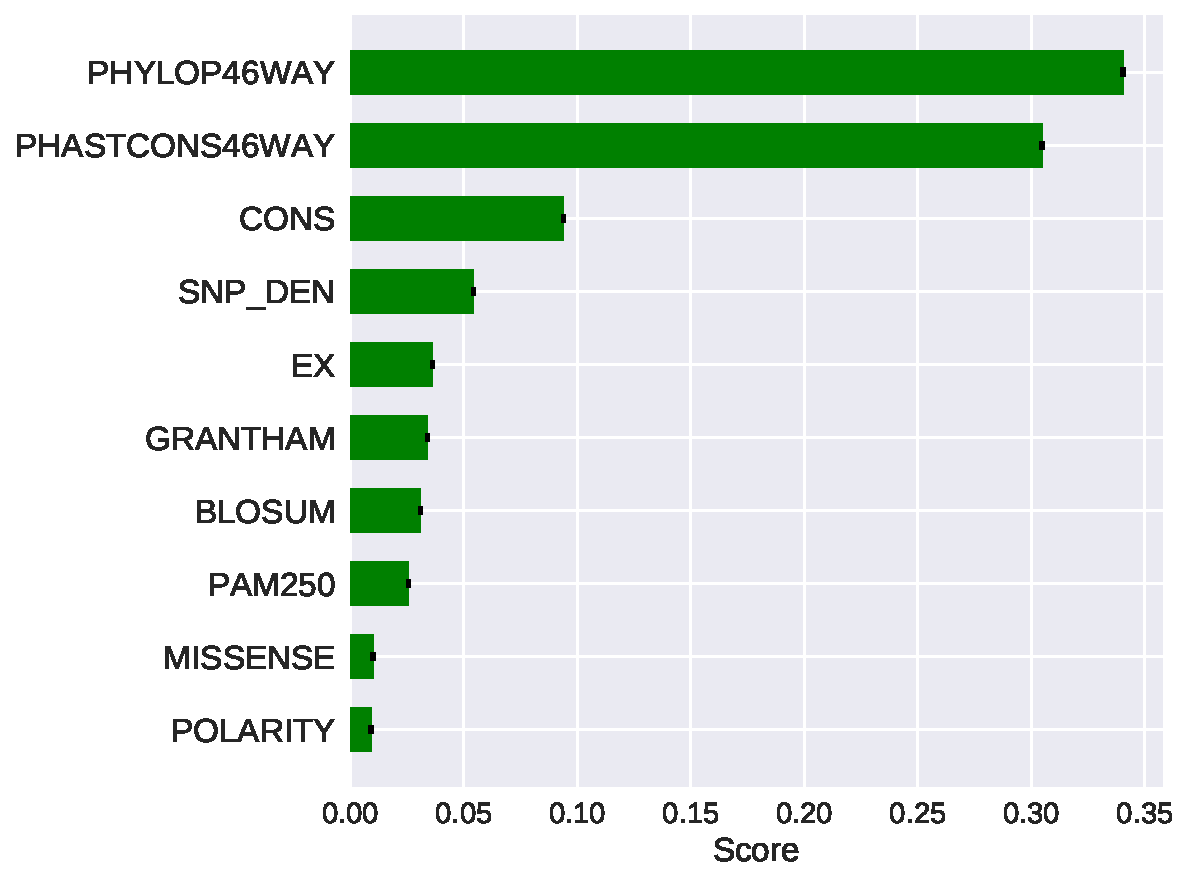
\includegraphics[width=\textwidth]{documents/latex/figures/3/integral/importances_integral.pdf}
    \caption{Los 10 atributos más importantes del dataset Integral aportados por el algoritmo Random Forest.}
    \label{fig:importances_integral_rf}
\end{subfigure}

\caption{Curva AUC y atributos más importantes de los modelos RF y XGBoost usando el dataset Integral.}

\end{figure}


\chapter{Integrando las nuevas variables al dataset VarQ Curado}
\label{ch:desarrollo_integral_varq}
% \section{Integrando las nuevas variables al dataset VarQ Curado}

En esta sección buscamos cuantificar en qué medida el esfuerzo realizado a lo largo de esta tesis mejora e impacta sobre nuestro set de datos original (VarQ). Para ello, integraremos al set VarQ Curado, que dispone de 9 features estructurales y 7,418 variantes, los features físico-químicos y genómicos obtenidos a lo largo de esta tesis.

\section{Creación del dataset Integral+VarQ Curado}
Para generar este dataset cruzamos las variantes de ambos datasets, haciendo un \textit{right-outer-join} (ver figura \ref{fig:interseccion_varq_integral}). Es decir que nos quedamos con las variantes de VarQ Curado a las que sumamos las variables del dataset Integral para aquellas variantes en la intersección de los dos conjuntos. El dataset resultante posee 73 variables, que corresponden a las 63 variables del dataset Integral sumado a las 9 variables del dataset VarQ Curado y la variable de respuesta. Este dataset posee 7,418 variantes de las cuales 5,377 (72\%) son patogénicas y 2,041 (28\%) son benignas. Las 774 variantes que no poseen variables del dataset Integral se mantuvieron en este nuevo dataset. Es por eso que en este caso la proporción de nulos para las variables genómicas es mayor que en el caso Integral, por un lado porque no se recomputaron esas variables para las variantes que no están en la intersección (774), si no que además dentro de la intersección con el dataset Integral, la cantidad de variantes sin cobertura genómica es de aproximadamente el 36\%, mientras que en el dataset Integral este valor llegaba al 20\%. Dejamos como trabajo futuro la generación de variables genómicas para las variantes de VarQ Curado no presentes en el dataset Integral.

\begin{figure}[H]
    \centering
    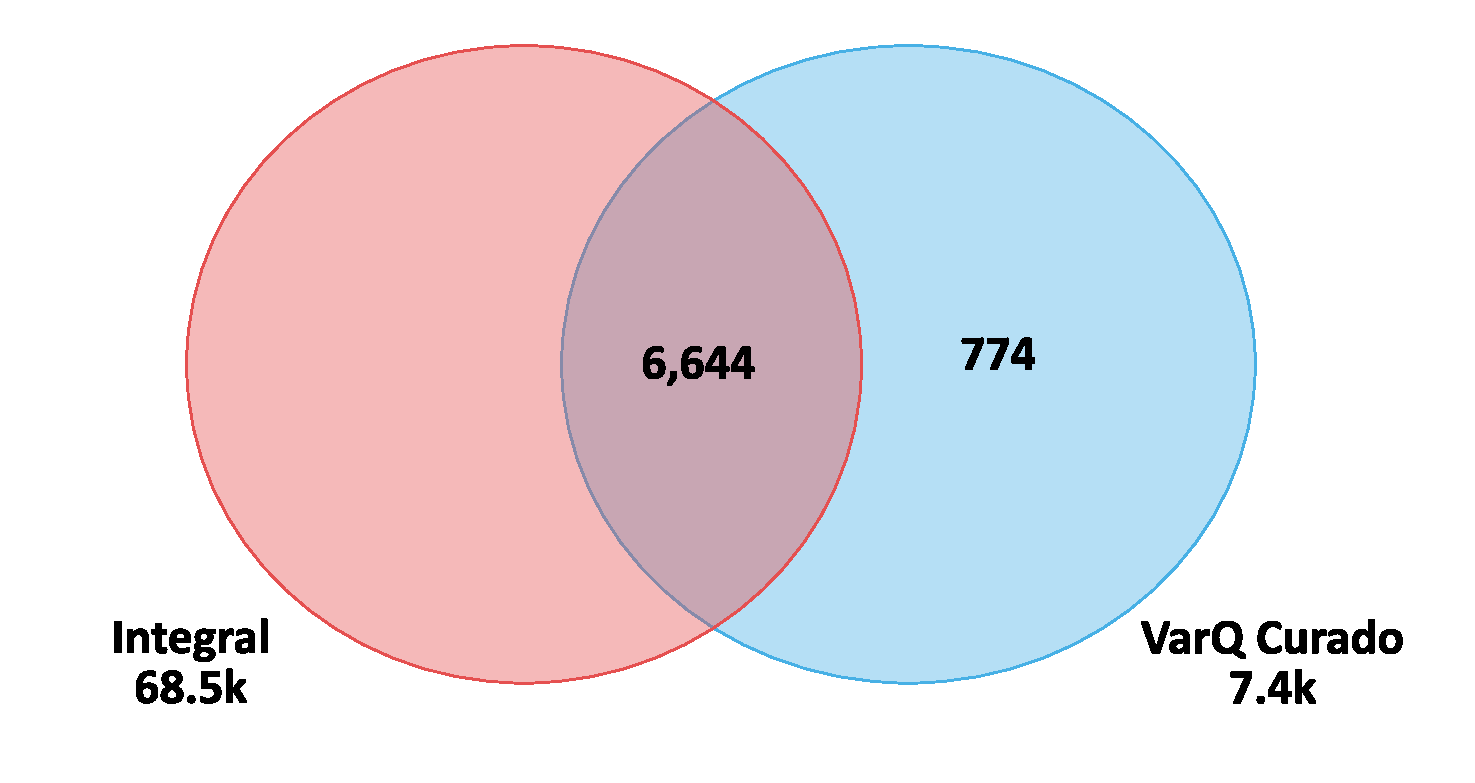
\includegraphics[scale=0.4]{documents/latex/figures/3/integral_varq/interseccion_varq_integral.pdf}
    \caption{Intersección entre los datasets Integral y VarQ Curado .}
    \label{fig:interseccion_varq_integral}
\end{figure}

\section{Generación del Modelo}
Como en los capítulos anteriores, se volvió a utilizar el Pipeline Tree para los modelos XGBoost y Random Forest. El dataset de entrenamiento posee 4,970 variantes (66\%), y el tercio restante se destinó al dataset de test. Estas variantes fueron elegidas al azar, con una semilla pseudoaleatoria para poder replicar el experimento. Este procedimiento se repitió en todos los modelos.  

\section{Resultados}
El dataset de test arrojó un AUC de 0.86 para Random Forest y 0.88 con XGBoost (ver figura \ref{fig:auc_integral_varq}). El test de DeLong \cite{DeLong} arrojó un p-valor menor a $2\mathrm{e}{-7}$, lo que nos permite aseverar que el modelo XGBoost es superior a Random Forest. Este resultado representa una mejora sensible con respecto al modelo realizado con el dataset VarQ Curado (0.74), sin superar lo obtenido por el dataset Integral (0.90 con XGBoost). Nuestra hipótesis es que esto se debe a la menor cobertura de las variables de conservación genómica. Los hiperparámetros de los modelos fueron, en el caso de Random Forest: Profundidad del árbol 7, 100 estimadores y Cantidad de variables por árbol 0.2*\textit{n} con \textit{n} la cantidad total de variables. En el caso de XGBoost, los hiperparámetros elegidos fueron:

\begin{itemize}
    \item \texttt{min\_child\_weight}: 5
    \item \texttt{gamma}: 1.5
    \item \texttt{subsample}: 1
    \item \texttt{colsample\_bytree}: 0.6
    \item \texttt{max\_depth}: 5
\end{itemize}

Considerando a la clase patogénica como clase positiva, vemos que XGBoost supera a RF en Precisión, AUC y F1-score, pero no en Recall (ver tabla \ref{tab:metrics_model_varq_integral}). Sin embargo, si tomamos a las clase benigna como positiva, el modelo XGBoost supera a RF (0.59 vs 0.53). Si bien sigue siendo un número bajo, es posible modificar el \textit{threshold} en la función de decisión en ambos modelos para obtener un Recall más alto sacrificando precisión. 

\begin{table}[H]
\centering
\begin{tabular}{|l|l|l|l|l|l|l|}
\hline
Modelo & Precisión & Recall & AUC & F1-score & $t_{fit}$ & $t_{pred}$ \\ \hline
RF  & 0.84 & 0.95 & 0.87 & 0.89 & 15.4 s & 0.07 s \\ \hline
XGBoost & 0.86 & 0.94 & 0.88 & 0.90 & 1m 20 s & 0.1 s \\ \hline
\end{tabular}

\caption{Comparación de métricas de modelos usando el dataset Integral+VarQ Curado. Las variables $t_{fit}$ y $t_{pred}$ corresponden al tiempo de entrenamiento y de predicción de todas las variantes.}
\label{tab:metrics_model_varq_integral}
\end{table}


\begin{table}[H]
\centering
\begin{tabular}{|l|l|l|l|}
\hline
             & Precision & Recall & F1-score \\ \hline
Benignas     & 0.81      & 0.53   & 0.64     \\ \hline
Patogénicas  & 0.84      & 0.95   & 0.89     \\ \hline
Promedio     & 0.83      & 0.83   & 0.82     \\ \hline
\end{tabular}
\caption{Reporte de métricas del modelo Random Forest usando el dataset Integral+VarQ Curado.}
\label{tab:metrics_integral_varq_rf}
\end{table}


\begin{table}[H]
\centering
\begin{tabular}{|l|l|l|l|}
\hline
             & Precision & Recall & F1-score \\ \hline
Benignas     & 0.80      & 0.59   & 0.68     \\ \hline
Patogénicas  & 0.86      & 0.94   & 0.90     \\ \hline
Promedio     & 0.84      & 0.85   & 0.84     \\ \hline
\end{tabular}
\caption{Reporte de métricas del modelo XGB usando el dataset Integral+VarQ Curado.}
\label{tab:metrics_integral_varq_xgb}
\end{table}

\section{Importancia de las variables}
La información proporcionada por \texttt{scikit-learn} acerca de la importancia de las variables en el modelo Random Forest están presentadas en la figura \ref{fig:importances_integral_varq}. En este ranking de las 10 variables más relevantes encontramos otra vez en primer lugar con amplia ventaja a las variables de conservación genómica, aunque también se mantiene la variación de energía y al porcentaje de SASA, que son variables pertenecientes al dataset VarQ Curado y que habían aparecido en el ranking de dicho modelo. Si consideramos la variaciones en la precisión de los modelos Random Forest y XGBoost calculados por el módulo \texttt{rfpimp} (ver figuras \ref{fig:importance_cluster_integral_varq} y \ref{fig:importance_cluster_integral_varq_xgb}), encontramos nuevamente a SNP\_DEN como una variable relevante en el modelo XGBoost, mientras que en el modelo RF aparece en el cuarto puesto con escasa diferencia de las variables con menor relevancia. VARIATION\_ENERGY y las matrices (GRANTHAM, EX, PAM250, etc.) aparecen en ambos modelos como relevantes. 


% Side by side figures 
\begin{figure}[H]
\begin{subfigure}[c]{0.50\linewidth}
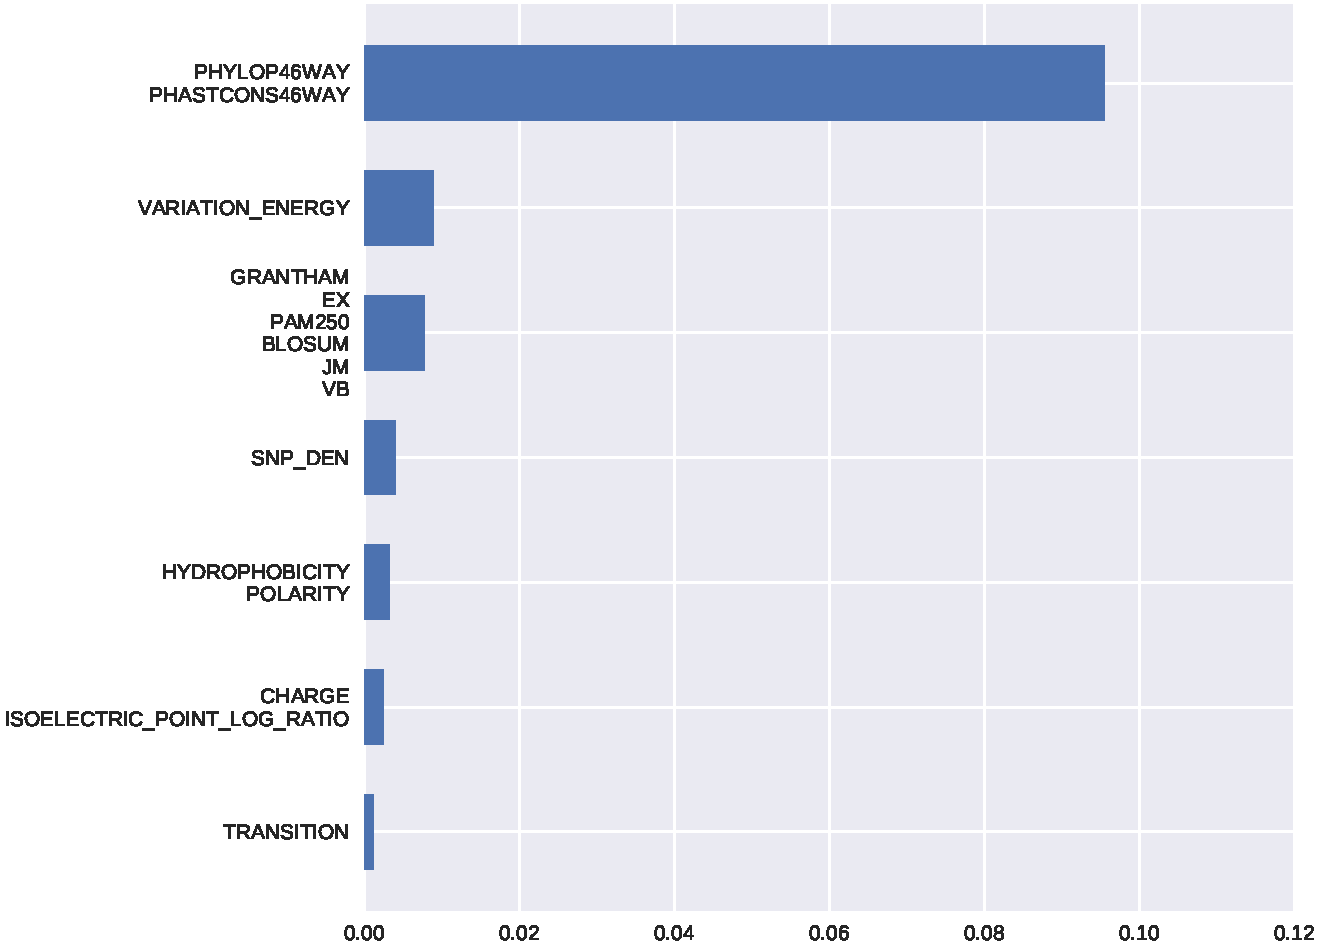
\includegraphics[width=\linewidth]{documents/latex/figures/3/integral_varq/integral_varq_importance_cluster.pdf}
\caption{Resultados del modelo usando RF.}
\label{fig:importance_cluster_integral_varq}
\end{subfigure}
% \hfill
\begin{subfigure}[c]{0.45\linewidth}
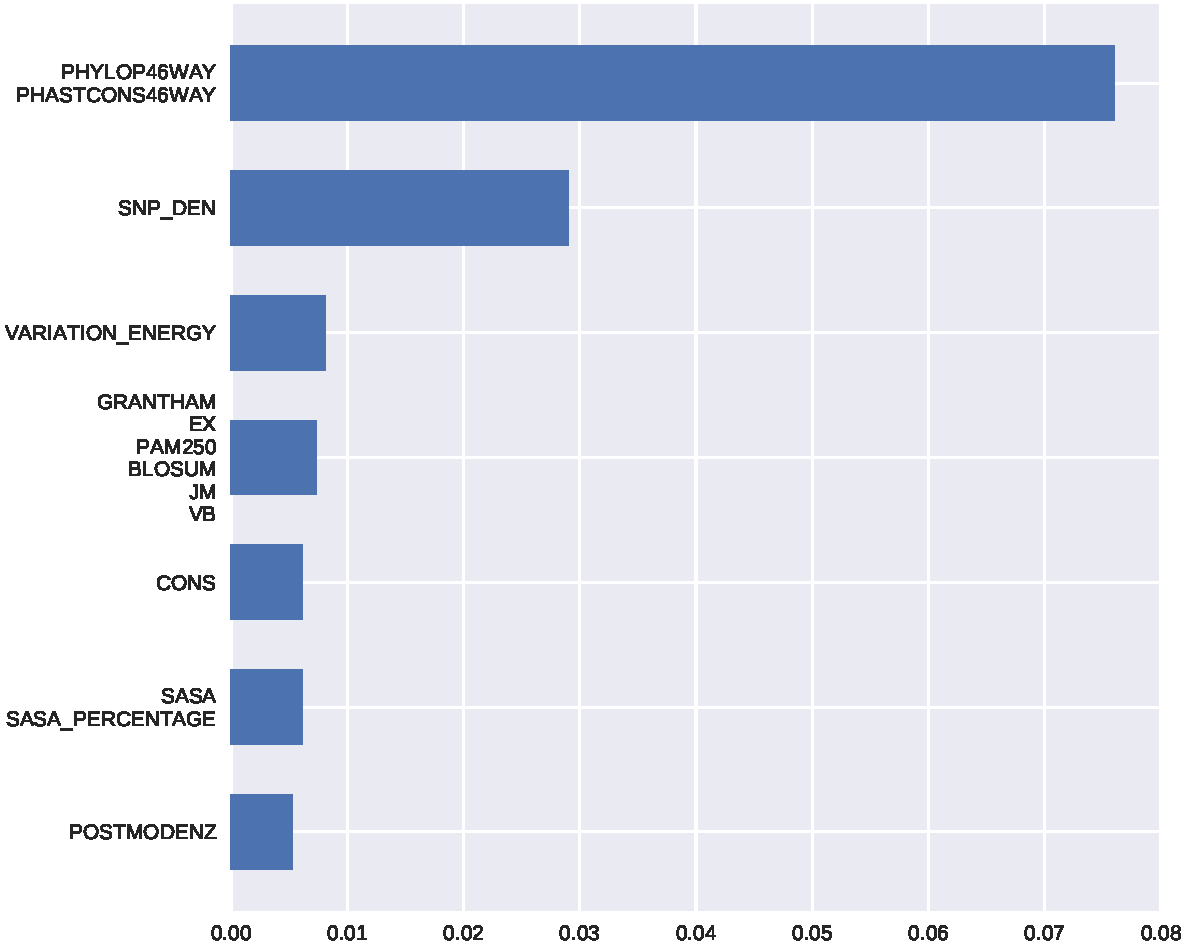
\includegraphics[width=\linewidth]{documents/latex/figures/3/integral_varq/integral_varq_importance_cluster_xgb.pdf}
\caption{Resultados del modelo usando XGB.}
\label{fig:importance_cluster_integral_varq_xgb}
\end{subfigure}%
\caption{Importancia de variables altamente correlacionadas del dataset Integral+VarQ Curado (basados en correlación de Spearman) usando permutación.}
\end{figure}



\section{Conclusión del capítulo}

La creación de un modelo combinando los datos de VarQ Curado con los del dataset Integral no superó lo obtenido por éste, aunque creemos que es posible mejorar este resultado calculando tanto las variables más importantes de VarQ (VARIATION\_ENERGY y SASA) para las variantes del dataset Integral, como las variables genómicas para las variantes del dataset VarQ Curado. 

\newpage
\begin{figure}[H]
\centering
\begin{subfigure}[b]{0.7\textwidth}
    \centering
    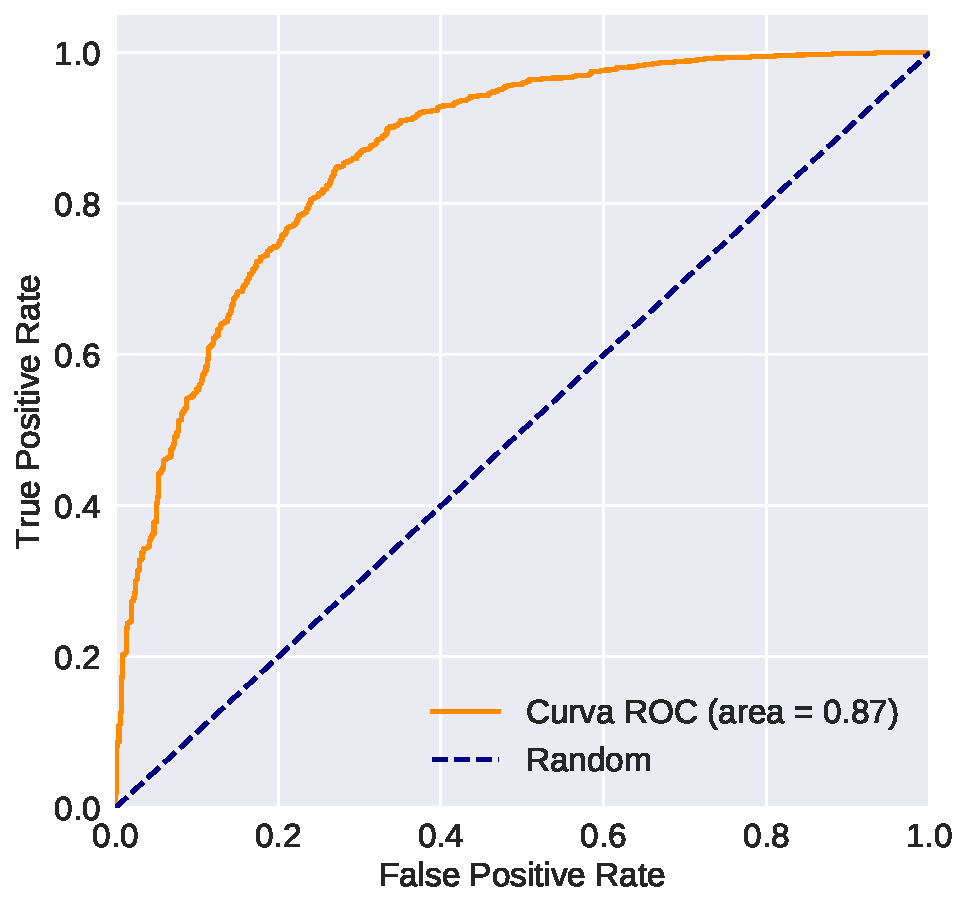
\includegraphics[width=\textwidth]{documents/latex/figures/3/integral_varq/auc_varq_integral.pdf}
    \caption{Curva AUC de los modelos Random Forest y XGBoost. La línea punteada corresponde a un predictor Random.}
    \label{fig:auc_integral_varq}
\end{subfigure}
\hfill
\hfill
\begin{subfigure}[b]{0.7\textwidth}
    \centering
    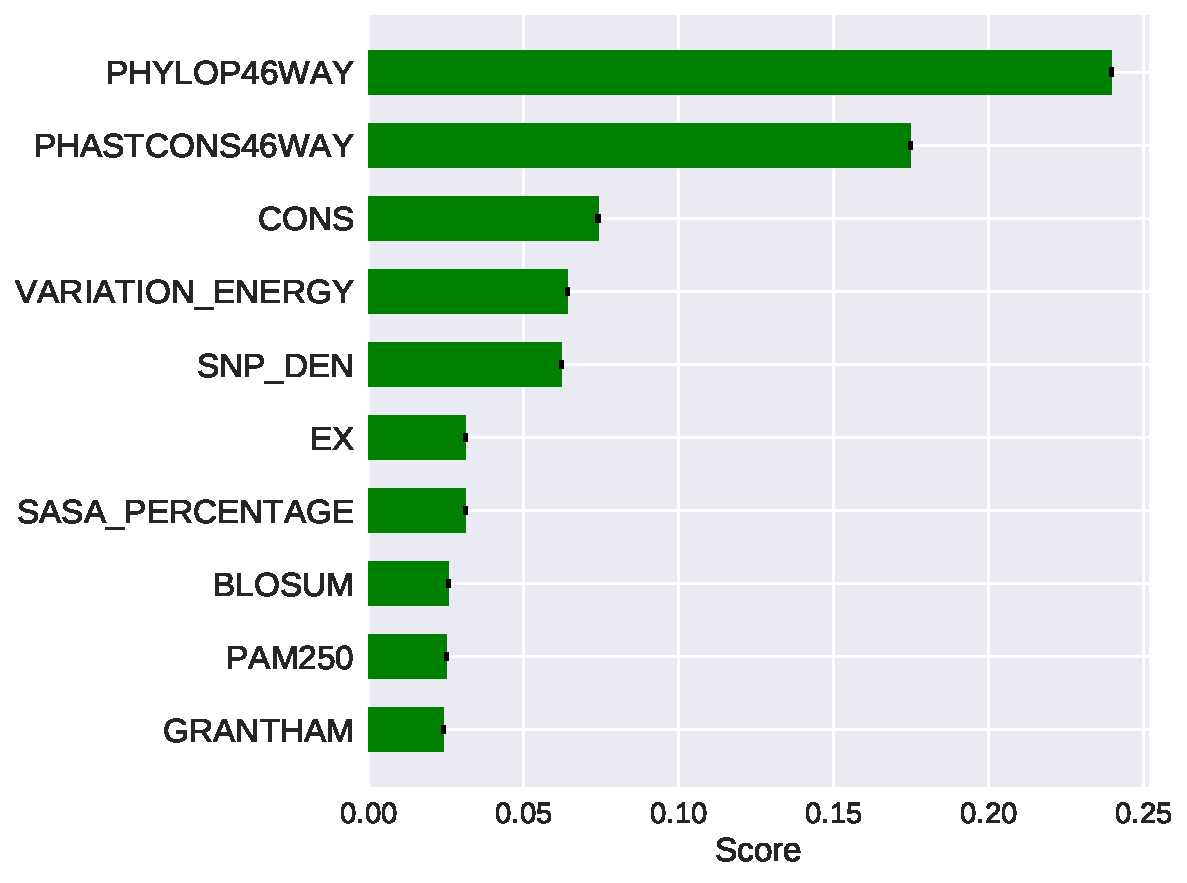
\includegraphics[width=\textwidth]{documents/latex/figures/3/integral_varq/importances_varq_integral.pdf}
    \caption{Los 10 atributos más importantes del modelo Random Forest.}
    \label{fig:importances_integral_varq}
\end{subfigure}

\caption{Curva AUC y atributos más importantes del dataset Integral+VarQ Curado.}
\end{figure}




\chapter{Conclusiones generales y trabajo futuro}
\label{ch:conclusiones}
En el presente trabajo mejoramos el modelo original pasando de un AUC de 0.74 a 0.90. Pero además hemos explorado diferentes aristas relativas al problema de predicción planteado con el objetivo de responder nuestros interrogantes iniciales. 

La primera pregunta era acerca de la posibilidad de enriquecer el dataset VarQ con nuevas fuentes de datos. Esta pregunta fue respondida afirmativamente, dado que agregar nuevas dimensiones demostró ser efectivo en la mejora del modelo, manteniendo fijo el algoritmo utilizado, siendo este Random Forest en todos los casos. En particular, el modelo que usó variables genómicas, arrojó un AUC de 0.85. El otro conjunto de variables analizado, las Físico-Químicas alcanzaron un AUC de 0.72. Si bien el AUC no fue superior al del modelo VarQ Curado, este demostró ser de utilidad. El modelo Integral, que combinó ambos datasets, resultó ser mejor que los dos anteriores, llegando a un AUC de 0.88 (figura \ref{fig:curvas_auc_humsavar}). Por último, sumar estas variables al dataset VarQ Curado también mostró una mejora, pasando de un AUC de 0.74 a 0.86 (figura \ref{fig:curvas_auc_varq}). 

La segunda pregunta que nos hicimos al comienzo del trabajo era sobre cómo la las variables afectan a nuestros modelos. La descripción estadística del dataset nos permitió entender como el método estándar para calcular importancia de variables en métodos de ensamble se ve afectado en variables altamente correlacionadas. Con respecto a las variables utilizadas, detectamos que las variables de conservación (phastCons y phyloP) son las más relevantes para nuestro problema de predicción. Si bien el dataset VarQ ya poseía variables de conservación, estas pertenecen a familias de proteínas (Pfam). Otras variables de importancia considerable son la variación de la energía (del dataset VarQ, obtenida vía PDB) y las matrices de sustitución o distancia (GRANTHAM, PAM250, BLOSUM, EX, JM y VB). Un aspecto destacable es que esta lista de variables corresponden a datasets distintos, reforzando la conclusión sobre la importancia de sumar dimensiones al problema.

Este trabajo también consistió en una comparación de distintos métodos de aprendizaje automático. En la primera sección del desarrollo comparamos tres métodos clásicos con el dataset VarQ Curado: Regresión Logística, Support Vector Classifier y Random Forest, obteniendo mejores resultados con éste último. Luego en la última sección del trabajo comparamos Random Forest con un método más avanzado de ensamble, XGBoost en los datasets Integral, mejorando la performance del modelo de un AUC de 0.88 a 0.90; y VarQ+Integral, llevando el AUC de 0.86 a 0.88.

\section{Trabajo Futuro}

Uno de los principales productos de este trabajo es la generación de un nuevo dataset que contiene numerosas variables estructurales y físico-químicos de la proteína, sumados a variables de tipo genómico. Este dataset también contiene variantes que están ligados a diferentes genes, que a su vez poseen cantidades distintas de SNPs potencialmente dañinos. Una de los trabajos que quedaron pendientes consisten en generar modelos individuales para cada gen, dado que puede existir un sesgo en nuestro modelo en caso de tener un número muy grande de SNPs de un gen determinado. También creemos que los trabajos futuros que deriven de este deberían hacer énfasis en la generación de modelos que mejoren la selección de hiperparámetros (en particular sugerimos el uso de técnicas de optimización bayesiana), y un tratamiento de nulos en variables categóricas más avanzado en comparación al usado en este trabajo. 

\begin{figure}[H]
\centering
\begin{subfigure}[b]{0.6\textwidth}
    \centering
    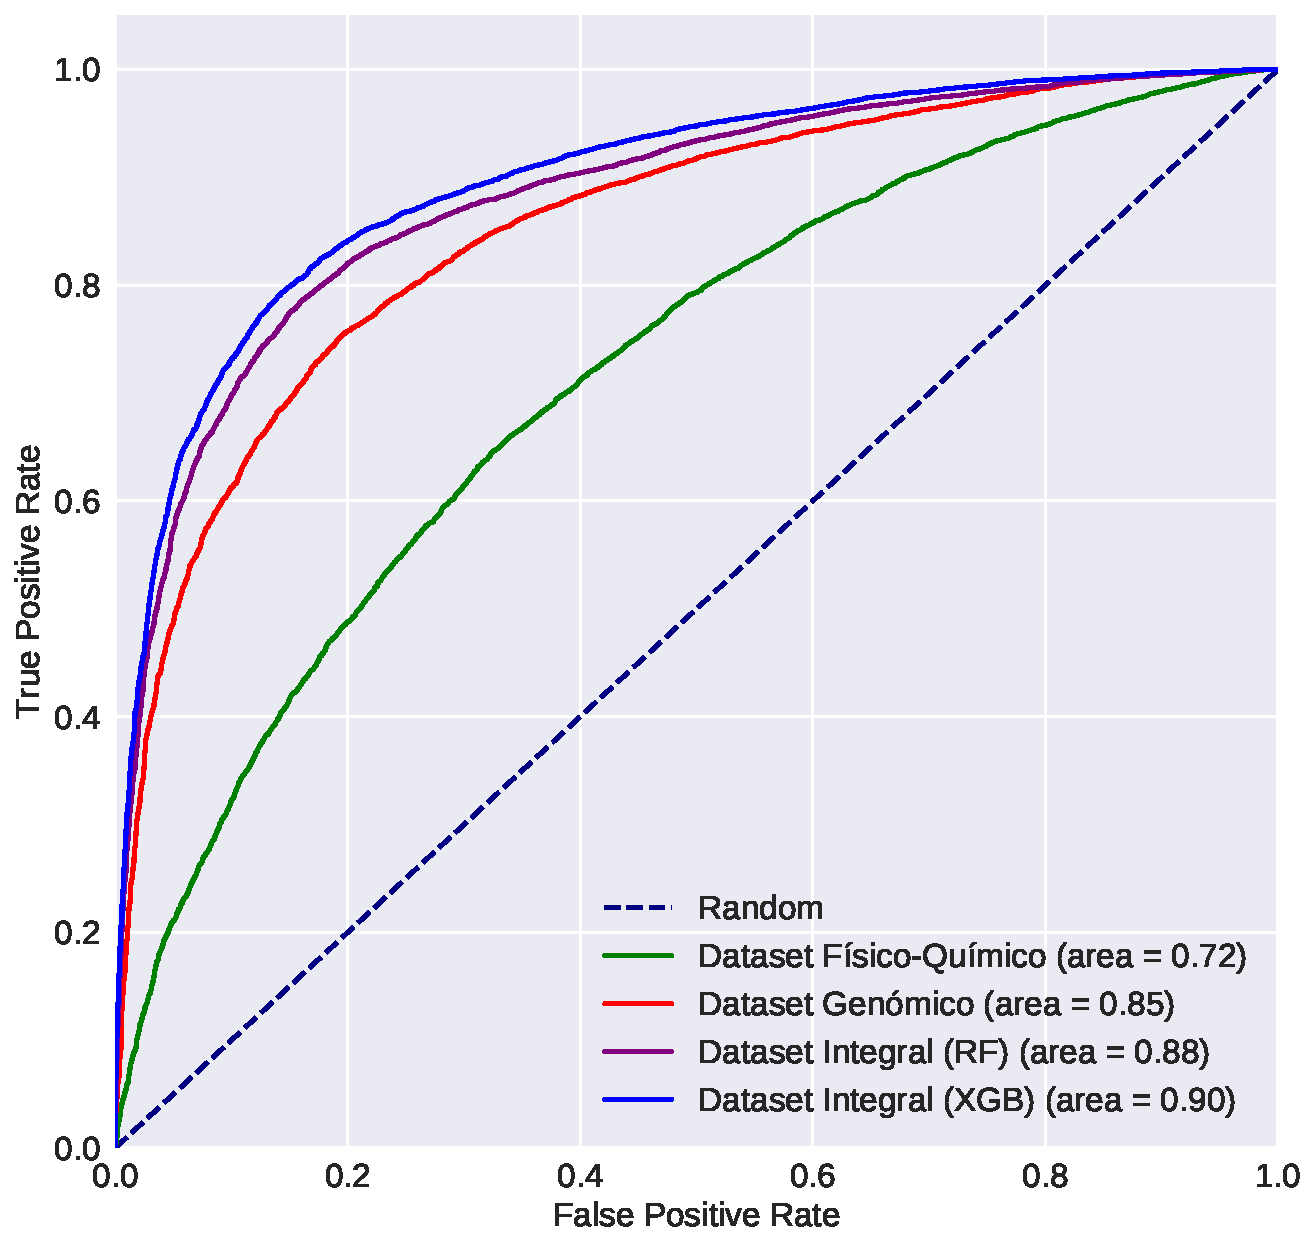
\includegraphics[width=\textwidth]{documents/latex/figures/4/curvas_auc_humsavar.pdf}
    \caption{Comparación de curvas ROC entre los datasets Físico-Químico, Genómico e Integral.}
    \label{fig:curvas_auc_humsavar}
\end{subfigure}

\hfill
\hfill

\begin{subfigure}[b]{0.6\textwidth}
    \centering
    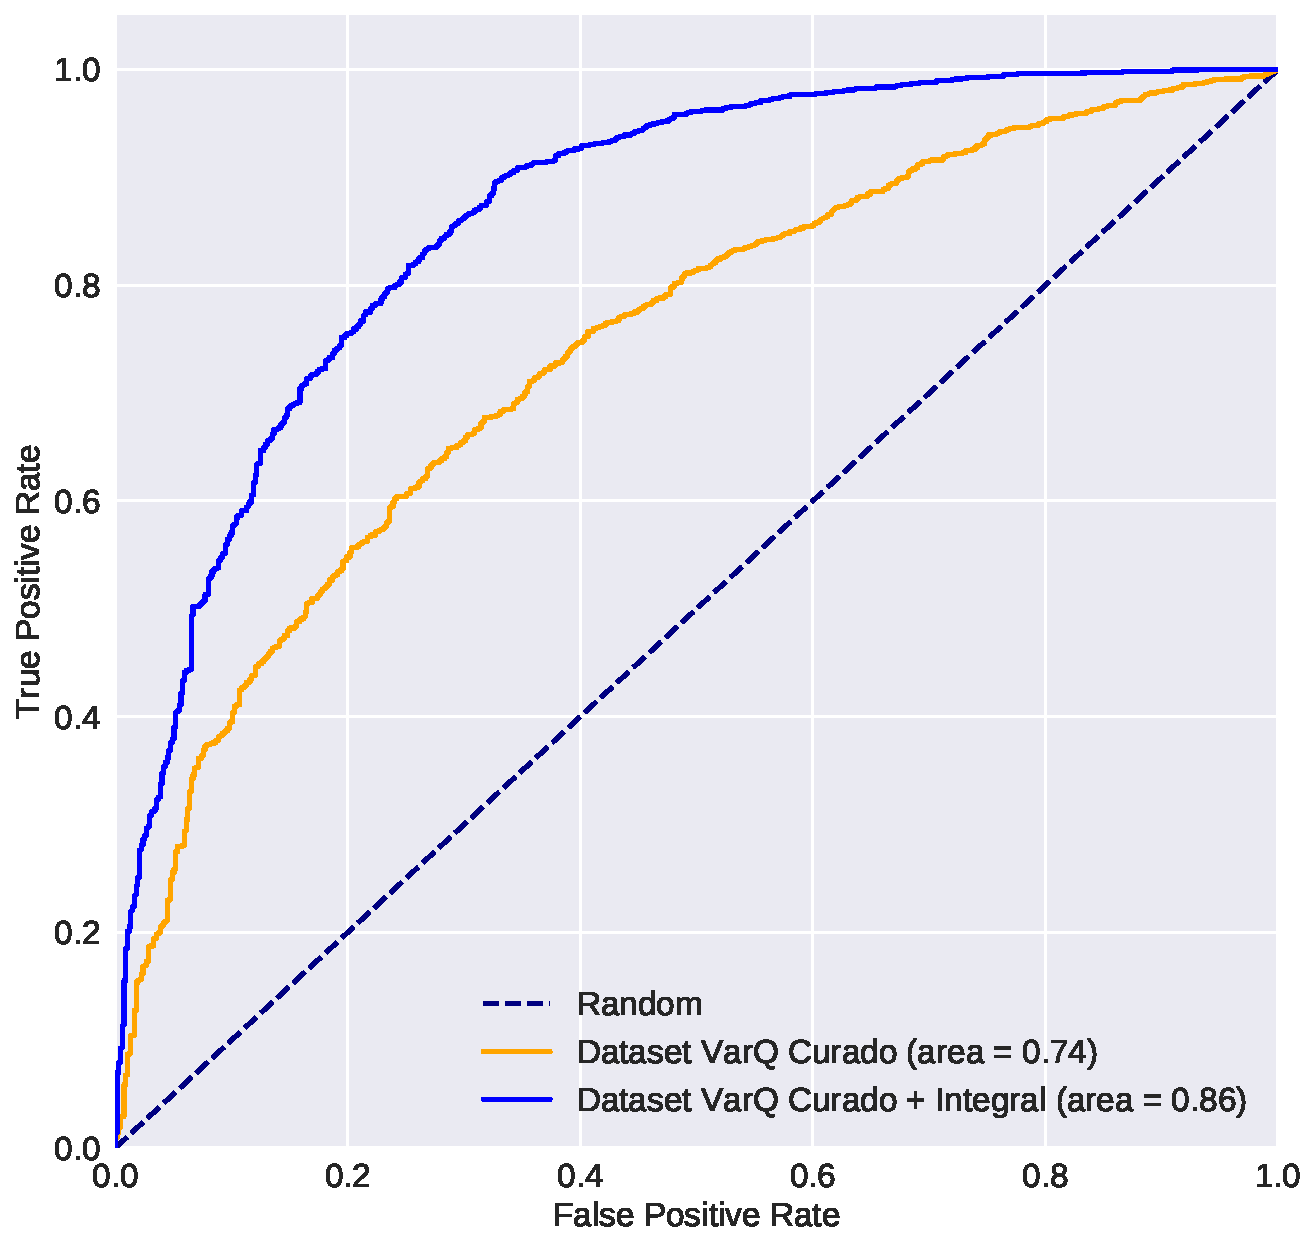
\includegraphics[width=\textwidth]{documents/latex/figures/4/curvas_auc_varq.pdf}
    \caption{Comparación de curvas ROC entre los datasets VarQ Curado y VarQ Curado + Integral.}
    \label{fig:curvas_auc_varq}
\end{subfigure}

\caption{Comparación de curvas AUC usando datasets con variantes de Humsavar y VarQ Curado.}
\end{figure}




%%%% BIBLIOGRAFIA

\backmatter

\bibliography{references/reference}
\addcontentsline{toc}{chapter}{Bibliografía}

\bibliographystyle{babunsrt}

\chapter{Apéndice}
\label{ch:apendice}
\section{Estructura del proyecto}

A continuación detallamos los distintos módulos del proyecto para facilitar la replicación de los resultados obtenidos. Este se encuentra alojado en GitHub. 

El proyecto tiene la siguiente estructura:

\vspace{0.2cm}
\dirtree{%
.1 master-thesis.
.2 data.
.2 notebooks.
.2 results.
.3 varq.
.3 physico\_chemical.
.3 genomic.
.3 integral.
.3 varq\_integral.
.2 src.
.3 snvbox\_queries.
}
\vspace{0.2cm}

En \texttt{src} se encuentra el código necesario para obtener las variables de la tabla SNVbox y generar las variables a partir de la data externa (por ejemplo, Humsavar) que se encuentra en la carpeta \texttt{data}. Luego, para cada modelo existe una notebook para generar el dataset y otro para evaluar los algoritmos, que almacenan los resultados en \texttt{results}. 


\section{Diccionario de hiperparámetros usados}

Para los modelos usados, se usaron los siguientes diccionarios de parámetros:
\begin{itemize}
    \item Random Forest
        \begin{itemize}
            \item Profundidad del árbol: [3, 5, 7]
            \item Estimadores: [10, 50, 100]
            \item Cantidad de variables por árbol: [4, $\sqrt{n}$, $0.2*n$] con n la cantidad total de variables
        \end{itemize} 
    \item Regresión logística:
        \begin{itemize}
            \item Parámetro de regularización inverso (C): [.001, .01, .1, 1, 10, 100, 1000]
            \item Peso de las clases: [balanceado, igual a 1]
        \end{itemize}
    \item SVC:
        \begin{itemize}
            \item Parámetro de penalidad (C): [0.001, 0.10, 0.1, 10, 25, 50, 100, 1000]
            \item Gamma: [0.001, 0.10, 0.1, 10, 25, 50, 100, 1000]
        \end{itemize}
    \item XGBoost:
        \begin{itemize}
            \item Peso mínimo de las hojas: [1, 5, 10]
            \item Gamma: [0.5, 1, 1.5, 2, 5]
            \item Subsample: [0.6, 0.8, 1.0]
            \item colsample\_bytree: [0.6, 0.8, 1.0]
            \item Profundidad máxima: [3, 4, 5]
        \end{itemize}
\end{itemize}


\section{Lista de Variables de SNVBox}

\subsubsection{Variables sobre cambios en la sustitución del Aminoácido (Estructura Primaria)}
\begin{itemize}
    \item Score BLOSUM (AABLOSUM): Score de la matriz BLOSUM 62.
    \item Carga (AACharge): El cambio en la carga resultante de cambiar el aminoácido de referencia con la mutación.
    \item Volumen (AAVolume): El cambio en el residuo resultante del cambio de aminoácido (expresado en Angstroms cúbicos).
    \item Hidrofobia (AAHydrophobicity): El cambio en hidrofobicidad resultante de la mutación.
    \item Score Grantham (AAGrantham): La distancia Grantham de la referencia a la mutación.
    \item Polaridad (Polarity): Cambio de polaridad entre la referencia y la mutación.
    \item Score Ex (AAEx): Score de la matriz EX.
    \item Score PAM250 (AAPAM250): Score de la matriz PAM250.
    \item Score MJ (AAMJ): Score de la matriz Miyagawa-Jerningan.
    \item Score HGMD2003 (AAHGMD2003): Número de veces que la sustitución ocurre en la base de datos HGMD.
    \item Score VB (AAVB): Score de la matriz VB (Venkatarajan \& Braun).
    \item Transición (Transition): Frecuencia de la transición entre dos aminoácidos vecinos basado en todas las proteínas de SwissProt/TrEMBL.
    \item COSMIC: Frecuencia de cambio \textit{missense} en la base COSMIC.
    \item COSMICvsSWISSPROT: Frecuencia de cambio \textit{missense} sobre la cantidad de proteínas en SwissProt.
    \item HAPMAP: Cantidad de sustituciones en HAPMAP.
    \item COSMICvsHAPMAP: Frecuencia de cambio \textit{missense} sobre la cantidad de proteínas en HAPMAP.
\end{itemize}

\subsubsection{Variables a nivel de Proteína (sin considerar sustitución)}

\begin{itemize}
    \item BINDING: Sitio de unión.
    \item ACTIVE\_SITE: Actividad enzimática. 
    \item SITE: Sitio ``interesante''.
    \item LIPID: Unión con un lípido.
    \item METAL: Unión con un metal.
    \item CARBOHYD: Unión con un carbohidrato.
    \item DNA\_BIND: Unión con ADN.
    \item NP\_BIND: Unión con un nucleótido fosfato.
    \item CA\_BIND: Unión con calcio.
    \item DISULFID: Sitio de unión con un disulfuro.
    \item SE\_CYS: Selenocisteína.
    \item MOD\_RES: Residuo modificado.
    \item PROPEP: Propéptido.
    \item SIGNAL: Sitio de señal de localización.
    \item TRANSMEM: Proteína transmembranal.
    \item COMPBIAS: Sesgo de composición.
    \item REP: Región de repetición.
    \item MOTIF: Sitio de un motif funcional conocido.
    \item ZN\_FING: Dedo de zinc.
    \item REGIONS: Región de interés en la secuencia proteica.
    \item PPI: Interacción proteína-proteína.
    \item RNABD: Unión RNA.
    \item TF: Factor de transcripción. 
    \item LOC: Sitio que determina correcta localización celular de una proteína. 
    \item MMBRBD: Sitio que se une a la membrana celular.
\end{itemize}

% \vspace{2mm}
% \todo{
% TODO:
% Diagrama de SNVBOX
% }
% \vspace{2mm}

\end{document}
